%%%%%%%%%%%%%%%%%%%%%%%%%%%%%%%%%%%%%%%%%%%%%%%%%%%%%%%%%%%%%%%%%%%%%%%%%%%%%
% 1- INICIALITZACIÓ
%%%%%%%%%%%%%%%%%%%%%%%%%%%%%%%%%%%%%%%%%%%%%%%%%%%%%%%%%%%%%%%%%%%%%%%%%%%%%

\documentclass[catalan,final]{../latex-manual-template/manual_template}
% \usepackage{etoolbox}
\usepackage[super]{nth}
\usepackage[sort,nocompress]{cite}
\usepackage{tikz}
\usetikzlibrary{shapes.geometric, arrows}

\tikzstyle{startstop} = [rectangle, rounded corners, minimum width=3cm, minimum height=1cm,text centered, text width=3cm, draw=black, fill=white]
\tikzstyle{io} = [trapezium, trapezium left angle=70, trapezium right angle=110, minimum width=3cm, minimum height=1cm, text centered, text width=2.8cm , draw=black, fill=white]
\tikzstyle{process} = [rectangle, minimum width=3cm, minimum height=1cm, text centered, text width=3cm, draw=black, fill=white]
\tikzstyle{decision} = [diamond, minimum width=2cm, minimum height=1cm, text centered, text width=2cm, draw=black, fill=white]
\tikzstyle{arrow} = [thick,->,>=stealth]


\usepackage{tikz-qtree} % Tree diagram
\usepackage{circuitikz} % Electrical circuits
\usepackage{enumitem}   % Introduce lists of items

% \usepackage{subcaption}
\usepackage[font={small,it},labelfont=bf]{caption}
% \usepackage[labelfont=bf]{caption}
\usepackage{float}
% \usepackage{subfloat}

% \usepackage{mwe}
% \usepackage{subfigure}
\usepackage{subfigure}

\usetikzlibrary{trees}
\usetikzlibrary{shadows}

\usepackage{color, colortbl}
\usepackage{pbox}
\usepackage{bm} % Provide bold maths symbols
\usepackage{graphicx}
\graphicspath{/images/}
\addtolength{\footnotesep}{1mm} % change to 1mm
\interfootnotelinepenalty=10000 % Avoid to break a footnote into two different pages



%% * OPCIONS A CONFIGURAR al \documentclass
%%    - Estat del document: final o draft
%%      NOTA: Draft no inserta les figures i marca només l'espai que
%%      ocupen. També s'indica quan el text sobrepassa els marges.
%%      Draft és molt útil per compilar ràpid el document si no és important
%%      en aquell moment visualitzar les figures.
%%    - Idioma PRINCIPAL del document: catalan, spanish, english, french...

\usepackage[english]{babel}
%%    NOTA: per canviar d'idioma al mig del document usar:
%%          \selectlanguage{nom_idioma}
%%%%%%%%%%%%%%%%%%%%%%%%%%%%%%%%%%%%%%%%%%%%%%%%%%%%%%%%%%%%%%%%%%%%%%%%%%%%%

%%%%%%%%%%%%%%%%%%%%%%%%%%%%%%%%%%%%%%%%%%%%%%%%%%%%%%%%%%%%%%%%%%%%%%%%%%%%%
% 2- CÀRREGA DE PAQUETS ADICIONALS (OPCIONALS)
%%%%%%%%%%%%%%%%%%%%%%%%%%%%%%%%%%%%%%%%%%%%%%%%%%%%%%%%%%%%%%%%%%%%%%%%%%%%%

\usepackage[utf8]{inputenc}
\DeclareUnicodeCharacter{00A0}{ }
\usepackage{amssymb,amsmath, amsfonts}  %% Símbols matemàtics de la American Mathematical Society  
\usepackage{array}                      %% El paquet array proporciona eines molt útils a l'hora de fer equacions amb matrius       
\usepackage{multirow}                   %% Paquet que permet fer taules fusionant cel·les de files consecutives          
\usepackage{longtable}                  %% Paquet molt útil en cas de tenir taules molt llargues que ocupin vàries pàgines          
\usepackage{cases}                      % Two different labeled equations (warning: tiene que ir detras de 'ansmath')
\usepackage{tablefootnote}
\usepackage{pdfpages}

\usepackage[framed,numbered,autolinebreaks,useliterate]{mcode}



%% Paquet molt útil que permet activar links en el PDF final.
%% * NO OBLIDAR DE CONFIGURAR els quatre primer camps!
\usepackage[
  pdfauthor={Nom Cognoms autor},            % Configurar adientment
  %pdftitle={Treball Fi de Carrera - autor}, % Configurar adientment
  %pdfsubject={Titol del TFC aqui},          % Configurar adientment
  % Modificació respecte a la versió 2.1 - Iván Padilla Montero - Juliol 2014
  pdftitle={Treball Fi de Grau - autor}, % Configurar adientment
  pdfsubject={Titol del TFG aqui},          % Configurar adientment  
  pdfkeywords={keyword1, keyword2, ...},    % Configurar adientment
  pdfcreator={EETAC-UPC}, 
  pdfproducer={LaTeX, dvipdf},
  pdfdisplaydoctitle=true, plainpages=false, linktocpage=true,         
  colorlinks=true, linkcolor=blue,citecolor=blue,urlcolor=blue,
  hyperfootnotes=false, pagebackref=true, pdfpagelabels=true,            % PARA NO PONER NUMERO DE PAGINA EN LA REFERENCIA
  pdfpagemode=UseOutlines,
]{hyperref} 

\usepackage{layout}
\usepackage{showframe}
\usepackage[export]{adjustbox}

%% NOTA IMPORTANT!:
%% Per tal que hyperef funcioni correctament amb els capitols o seccions no
%% numerats (\chapter*{}), com per exemple introducció, conclusions i bibliografia
%% cal posar les dues comandes seguents ABANS del \chapter*{} en questió
%\cleardoublepage
%\phantomsection

%% Permet trencar links URL. 
%% Atenció! afegir aquest paquet DESPRES del hyperref!!
%\usepackage{breakurl} 

%% Permet arranjar matricialment multiples figures
%% NOTA: afegir aquest paquet DESPRES del hyperref!!
%%       Si no es desitja utilitzar aquest paquet, comentar la linia seguent
%%       i anar TAMBE al fitxer de classe (eetac_tfc_pfc.cls) per substituir: 
%%       \RequirePackage[subfigure]{tocloft}  per  \RequirePackage{tocloft}
\usepackage{subfigmat}     
% \usepackage{showframe,subcaption}
%%%%%%%%%%%%%%%%%%%%%%%%%%%%%%%%%%%%%%%%%%%%%%%%%%%%%%%%%%%%%%%%%%%%%%%%%%%%%
% 3- DOCUMENT
%%%%%%%%%%%%%%%%%%%%%%%%%%%%%%%%%%%%%%%%%%%%%%%%%%%%%%%%%%%%%%%%%%%%%%%%%%%%%

%%% Configuració de les dades i variables boleanes rellevants del document:
%%%%%%%%%%%%%%%%%%%%%%%%%%%%%%%%%%%%%%%%%%%%%%%%%%%%%%%%%%%%%%%%%%%%%%%%%%%%%
%%%%%%                                                                  %%%%% 
%%%%%%       Fitxer de dades per la memoria TFC/PFC de l'EETAC          %%%%% 
%%%%%%                                                                  %%%%% 
%%%%%%%%%%%%%%%%%%%%%%%%%%%%%%%%%%%%%%%%%%%%%%%%%%%%%%%%%%%%%%%%%%%%%%%%%%%%%


%%%%%%%%%%%%%%%%%%%%%%%%%%%%%%%%%%%%%%%%%%%%%%%%%%%%%%%%%%%%%%%%%%%%%%%%%%%%%%%
%%  VARIABLES A CONFIGURAR                                                  %%%
%%%%%%%%%%%%%%%%%%%%%%%%%%%%%%%%%%%%%%%%%%%%%%%%%%%%%%%%%%%%%%%%%%%%%%%%%%%%%%%

%% - Projecte o Treball de Fi de Carrera?
%%      PFC = true   -> Projecte de Fi de Carrera
%%      PFC = false  -> Treball  de Fi de Carrera
\setboolean{manual}{true}

%% - Escollir la titulació
%\titulacio{Enginyeria Tècnica Aeronàutica, especialitat Aeronavegació}
%\titulacio{Enginyeria T\`ecnica de Telecomunicaci\'o, especialitat Sistemes de Telecomunicaci\'o}
%\titulacio{Enginyeria T\`ecnica de Telecomunicaci\'o, especialitat Telem\`atica}
%\titulacio{Enginyeria de Telecomunicaci\'o (segon cicle)}
% Modificació respecte a la versió 2.1 - Iván Padilla Montero - Juliol 2014
%\titulacio{}
%\titulacio{Grau en Enginyeria d'Aeroports}
%\titulacio{Grau en Enginyeria Telemàtica}
%\titulacio{Grau en Enginyeria de Sistemes de Telecomunicació}


%% - Configurar els idiomes del document
%% Si l'idioma PRINCIPAL del document es l'angles, posar aquesta variable a true
\setboolean{Leng}{false}

%% Escollir entre catala i castella (idioma principial, o nomes pel resum en cas que l'idioma principal sigui anglès)
%%  catala = true   -> idioma principal (o només resum) en Català
%%  catala = false  -> idioma principal (o només resum) en Castella
\setboolean{Lcat}{true}

% Si les dues anteriors variables són falses, es posarà automàticament el títol en castellà
%\setboolean{Les}{false}

%% Titol del document en l'idioma principal del document 
\titol{MANUAL DE MUNTATGE D'UN QUADCOPTER}

%% Titol del document en anglès (Per l'apartat overview)
\titolE{QUADCOPTER DESIGN MANUAL}

%% Titol del document en catala/castella (Per l'apartat resum)
\titolC{MANUAL DE DISSENY I MUNTATGE D'UN QUADCOPTER}
\titolES{MANUAL DE DISEÑO DE UN QUADRICOPTERO}

%% - Nombre d'autors del TFC/PFC?
%%      UNautor = true   Un sol autor
%%      UNautor = false  Més d'un autor
\setboolean{UNautor}{true}

%% - Nom del(s) Autor(s) del document
%% NOTA: En cas de mes d'un autor cal posar la comana \and entre els
%%        noms dels autors
\autor{Llu\´is Hontecillas Guinart}

%% - Nombre de directors del TFC/PFC. Tipicament 1 o 2
%%      UNdirector = true   Un sol director
%%      UNdirector = false  Dos directors
%\setboolean{UNdirector}{true}

%% - Nom del Director del TFC/PFC
%\director{O}




%% - Es vol incloure una dedicatoria?
%%      dedicatoria = true   -> S'afegeix una pagina amb \textDedicatoria
%%      dedicatoria = true   -> No s'afegeix dedicatoria
%% NOTA: no confondre dedicatòria amb agraïments. Una dedicatoria sol ser
%%       un missatge curt d'una o dues frases màxim a la persona, o persones
%%       a les quals es dedica el treball. 
%%       Els agraïments poden ser extensos i l'autor pot agraïr a diverses
%%       persones coses diferents en funció de l'ajuda rebuda, per exemple. 
%%       Si es volen incloure agraïments, fer-ho al fitxer de la 
%%       memòria creant una secció nova amb  \chapter*{Agraïments}
%\setboolean{dedicatoria}{false}
%\textDedicatoria{}

%% - Es vol incloure una pagina d'index de figures?
%\setboolean{paginaLOF}{false}  % List of Figures

%% - Es vol incloure una pagina d'index de taules?
%\setboolean{paginaLOT}{falsa}  % List of Tables 

%% - El projecte ha estat supervisat per alguna persona externa? 
%%   (NOMES en cas de practiques en empresa)
%%      supervisor = true    -> Hi ha un supervisor
%%      supervisor = false   -> No hi ha un supervisor
%\setboolean{supervisor}{false}

%% NOMES en el cas de practiques en empresa (supervisor=true) s'han de 
%% configurar les variables seguents: 

%% Supervisor del TFC/PFC 
%\supervisor{Nom del Supervisor}

%% - Es vol incloure el logotip de l'empresa?
%%   En el cas que el TFC/PFC s'hagi fet en règim d'intercanvi amb una
%%   empresa, es pot afegir el seu logotip a la cantonada superior
%%   dreta de la portada. En aquest cas:
%%   - posar logo=true
%%   - posar el path de la imatge i l'alçada del logo a \mylogo
\setboolean{logo}{false}
\mylogo{./setup/drone_logo.png}{3.5cm}
  

%%% Configuració de MACROS o ENTORNS (opcionals) definides per l'usuari:
%%%%%%%%%%%%%%%%%%%%%%%%%%%%%%%%%%%%%%%%%%%%%%%%%%%%%%%%%%%%%%%%%%%%%%%%%%%%%
%%%%%%                                                                  %%%%% 
%%%%%%    Fitxer de macros d'usuari per la memoria TFC/PFC de l'EETAC   %%%%% 
%%%%%%                                                                  %%%%% 
%%%%%%%%%%%%%%%%%%%%%%%%%%%%%%%%%%%%%%%%%%%%%%%%%%%%%%%%%%%%%%%%%%%%%%%%%%%%%
%%%%%%%%%%%%%%%%%%%%%%%%%%%%%%%%%%%%%%%%%%%%%%%%%%%%%%%%%%%%%%%%%%%%%%%%%%%%%
%%                                                                         %%
%%         Author: Xavier Prats i Menendez (xavier.prats@upc.edu)          %% 
%%                  Technical University of Catalonia (UPC)                %%
%%                                                                         %%
%%%%%%%%%%%%%%%%%%%%%%%%%%%%%%%%%%%%%%%%%%%%%%%%%%%%%%%%%%%%%%%%%%%%%%%%%%%%%
%%      This work is licensed under the Creative Commons  Attribution-     %%
%%   -Noncommercial-Share Alike 3.0 Spain License. To view a copy of this  %% 
%%    license, visit http://creativecommons.org/licenses/by-nc-sa/3.0/es/  %%
%%    or send a letter to Creative Commons, 171 Second Street, Suite 300,  %%
%%                  San Francisco,California, 94105, USA.                  %%
%%%%%%%%%%%%%%%%%%%%%%%%%%%%%%%%%%%%%%%%%%%%%%%%%%%%%%%%%%%%%%%%%%%%%%%%%%%%%
%% Versio 1.5 - Juliol 2010                                                %%
%%%%%%%%%%%%%%%%%%%%%%%%%%%%%%%%%%%%%%%%%%%%%%%%%%%%%%%%%%%%%%%%%%%%%%%%%%%%%


%%% Xevi's macros for vectors and matrices:

%\newcommand{\ve}[1]{\mbox{\boldmath$#1$}}          
\newcommand{\ve}[1]{\vec{#1}}  
\newcommand{\ma}[1]{\mbox{\boldmath$\mathcal{#1}$}}

%%% Xevi's macros for brackets:
\newcommand{\lp}{\left(}
\newcommand{\lc}{\left[}
\newcommand{\lcl}{\left\{}
\newcommand{\rp}{\right)}
\newcommand{\rc}{\right]}
\newcommand{\rcl}{\right\}}

%%% Xevi's new environment for HIPOTESIS
\newcounter{num_hyp}
\newenvironment{hyp}[2]{
        \refstepcounter{num_hyp}
        \vspace*{2.5ex}
        {\noindent \bf\sffamily HYPOTHESIS #1 : #2} \\
        \sl
}
        {\vspace{1ex}
}

\newcommand{\SUMhyp}[2]{
 {\sffamily HYPOTHESIS #1 : #2} 
}
  

%%% Configuració manual de les regles d'hyphenation:
%%%%%%%%%%%%%%%%%%%%%%%%%%%%%%%%%%%%%%%%%%%%%%%%%%%%%%%%%%%%%%%%%%%%%%%%%%%%%
%%%%%%                                                                  %%%%% 
%%%%%%    Fitxer de hyphenation per la memoria TFC/PFC de l'EETAC       %%%%% 
%%%%%%                                                                  %%%%% 
%%%%%%%%%%%%%%%%%%%%%%%%%%%%%%%%%%%%%%%%%%%%%%%%%%%%%%%%%%%%%%%%%%%%%%%%%%%%%
%%%%%%%%%%%%%%%%%%%%%%%%%%%%%%%%%%%%%%%%%%%%%%%%%%%%%%%%%%%%%%%%%%%%%%%%%%%%%
%%                                                                         %%
%%         Author: Xavier Prats i Menendez (xavier.prats@upc.edu)          %% 
%%                  Technical University of Catalonia (UPC)                %%
%%                                                                         %%
%%%%%%%%%%%%%%%%%%%%%%%%%%%%%%%%%%%%%%%%%%%%%%%%%%%%%%%%%%%%%%%%%%%%%%%%%%%%%
%%      This work is licensed under the Creative Commons  Attribution-     %%
%%   -Noncommercial-Share Alike 3.0 Spain License. To view a copy of this  %% 
%%    license, visit http://creativecommons.org/licenses/by-nc-sa/3.0/es/  %%
%%    or send a letter to Creative Commons, 171 Second Street, Suite 300,  %%
%%                  San Francisco,California, 94105, USA.                  %%
%%%%%%%%%%%%%%%%%%%%%%%%%%%%%%%%%%%%%%%%%%%%%%%%%%%%%%%%%%%%%%%%%%%%%%%%%%%%%
%% Versio 1.5 - Juliol 2010                                                %%
%%%%%%%%%%%%%%%%%%%%%%%%%%%%%%%%%%%%%%%%%%%%%%%%%%%%%%%%%%%%%%%%%%%%%%%%%%%%%

\hyphenation{Cas-tell-de-fels}
\hyphenation{EETAC}
\hyphenation{MATLAB}
% http://dictionary.reference.com/browse/following  











\makeatletter
     \renewcommand*\l@figure{\@dottedtocline{1}{1em}{2.8em}}        % Let enough space after 2.1Figure of blablabla
     % \renewcommand*\l@figure{\@dottedtocline{1}{1em}{3.2em}} 
\makeatother



\begin{document}
\selectlanguage{catalan}
\beforepreface  

%% RESUM i OVERVIEW
%%%%%%%%%%%%%%%%%%%%%%%%%%%%%%%%%%%%%%%%%%%%%%%%%%%%%%%%%%%%%%%%%%%%%%%%%%%%%
% NOTA: les longituds passades com a parametres d'entrada  s'han
%        d'ajustar manualment fins que el requadre del resum/overview
%        ocupi tota la pàgina. 

%%% Resum en català (o castellà)
\selectlanguage{catalan}   
%\begin{resum}{10cm}
  
%E

%\end{resum}

%%% Resum en anglès
\selectlanguage{english}   
%\begin{overview}{11cm}


%\end{overview}


% Tornar a l'idioma principal del document
\selectlanguage{english}  
% Amb aqueta comanda indiquem que ja s'han inclòs tots els apartats del prefaci del 
% projecte o podem començar a incloure els capitols de la memòria
%\afterpreface


%%%%%%%%%%%%%%%%%%%%%%%%%%%%%%%%%%%%%%%%%%%%%%%%%%%%%%%%%%%%%%%%%%%%%%%%%%
%%%%%% INCLOURE A PARTIR D'AQUÍ TOTS ELS CAPÍTOLS DE LA MEMORIA   %%%%%%%%
%%%%%%%%%%%%%%%%%%%%%%%%%%%%%%%%%%%%%%%%%%%%%%%%%%%%%%%%%%%%%%%%%%%%%%%%%%

% NOTA: recordar que la introducció i les conclusions són capítols NO
%       enumerats, per tant s'ha d'usar \chapter*

% NOTA: és aconsellable incloure els capítols de la memòria en fitxers 
%       separats utlitzant la comanda \input  Per exemple:
%       \input{capitol1}  
%       que farà que s'inclogui el fitxer capitol1.tex

% NOTA: Si es vol incloure agraïments i/o glosari, fer-ho utilitzant 
% \chapter*{} i incloure'ls abans la introducció

\layout{}

Some text here to see the typography and hello world

\cleardoublepage
\phantomsection
\chapter{Introduction}

\section{Motivation of the Project}

In the last years, our society has experienced a silent, but intense trend towards autonomous electronic devices (e.g. laptops, digital cameras, smartphones, smartwatches, etc.) that we use in our daily life. In most cases, theses devices are powered by batteries, which need to be charged very often. Conventional recharges are made through the use of wires transmitting electrical energy from the generating point to the electrical device, but it has many problems related to alternating electric current while distribution. Even so, the greatest drawback is the lack of mobility. Moreover consumers have become inside a recharging lifestyle leaded by the combination of high-performance handheld electronics with a current battery technology uncapable to satisfy consumers' desire.

This fact motivated us to wonder whether there exist physical principles that could enable wireless powering of these and similar devices. Different technologies allow contactless energy transfer, each of them with their respective pros and cons. Recent investigations made us move towards inductive coupling systems due to its safety, lack of interference, and efficiency at medium ranges. 

\section{Objectives}
The aim of this project is to accomplish a brand new concept of inductive coupling implementing and outfitting the induction system on a nano-quadcopter with restrictive payload capabilities. A flying energy transporter widens the prospects and possibilities of unmanned aerial vehicles in such different fields, as aerospace, biomedical, multisensors, smart farming and robotics applications.

The study and modeling a resonant inductive system permits to design any inductive system by only having the requirements, such as power level or transfer distance. Based on different papers and projects, we decide to design the system with the purpose of transferring power up to 20 cm. This distance will constraint the dimensions of the inductive coils carried by the quadcopter.

One of the important goals of this project is to design and implement the inductive system inside a closed \textit{system} such as the nano-quadcopter. To achieve this, a strict calculation of performance and weight of each circuit should be made in order not to exceed the maximum take-off mass. 

Eventually, it is intended to demonstrate our system by powering a sensor, and also charging a small battery. Depending on the overall circuit efficiency and on the carrying energy, the transfer distance could be increased or reduced.  

\section{Brief History}\label{sec:timeline}

The idea of Wireless Power Transfer (WPT) is almost 200 years old. In 1826 Andre-Marie Ampere developed Ampere's circuital law, which shows the capacity of the electric current to produce a magnetic field. Five years later, Michael Faraday developed in England the Faraday's law of induction describing electromagnetic force can be induced in a conductor by a time-varying magnetic flux. In the United States Joseph Henry, independently to Faraday, discovers the same induced currents.\cite{keynote1}

In 1867 James Maxwell predicted the existence of electromagnetic waves. Twenty years later, the first spark transmitter generated a spark in a receiver that was several meters away from it. The German physicist Heinrich Hertz proved the existence of electromagnetic waves using this example \cite{2009wireless}.

The Serbian American inventor and engineer Nikola Tesla learned of Hertz's work by the following year and began duplicating his experiments.

In 1891, before the electrical-wire grid, Tesla proposed the first WPT theories \cite{meyer} carrying out various wireless transmission and reception experiments though air or matter. But, it was in 1894 when Tesla developed the equipment to wirelessly light incandescent lamps at his New York laboratory. This method used Resonant Inductive Coupling (RIC), which involves tuning two nearby coils to resonate at the same frequency. After this, no significant advances were made for more than 50 years. 

In 1969, Peter Glaser propose a transmission power link from space down the Earth. The project was named \textit{Solar Power Satellite} and it was based in harvesting solar radiation in space using satellites, which would convert it to microwave energy and then transmit it to Earth for use in electrical power systems.

In the early 1970s, experiments with RFID tags, done by the U.S. government \cite{RFID}, began and by the early 2000's the Professor She Yuen developed a charger to provide resonant power transfer for small electronics. 

Recently, in 2007 MIT researchers were able to power a 60 Watt light bulb from a power source while providing forty percent efficiency over distance in excess of two meters using RIC. Until that moment, the maximum transfer distances achieved between transmitter and receiver were on centimeter range scale. This event signified a turning point in WPT systems. In 2009 Sony showed a wireless electrodynamic-induction powered TV set, 60 V over 50 cm. Haier showed a wireless LCD TV at CES 2010 using researched Wireless Home Digital Interface \cite{medical}.

In July 2010 wireless charging technology for portable electronic devices up to 5 $W$ reached commercialization stage through the launch of the \textit{Qi} Standard by the Wireless Power Consortium, now comprising over 135 companies worldwide. Practically, it means that all receivers under \textit{Qi} specification can be supplied by all transmitters, signed with \textit{Qi} Standard, embracing compatibility between different devices.


\section{Category for the Wireless Power Transfer Systems} 

Wireless energy transfer systems, also called wireless power transfer (WPT), basically work by modulating the generated electric, magnetic, or electromagnetic fields to transport power from a transmitter towards a receiver at certain distance.

WPT systems can be cataloged by many ways, for example by the efficiency, power level, operating frequency, transmission distance, and so on. In this project, we classify the category of wireless power transfer systems by the working range. Figure \ref{fig:classification} shows the category.

As above figure shows, there are two basic sorts. They are the near-field transfers and the far-field transfers, since the field propagation behaviour and the consequent propagation losses strongly differ depending on the field region. 

In near-field or nonradiative region, the oscillating electric and magnetic fields are separate \cite{sazonov2014wearable} and power can be transferred via electric fields ($\vec{E}$) by capacitive coupling (electrostatic induction) or via magnetic fields ($\vec{B}$) by inductive coupling (electromagnetic induction) between coils of wire. These fields are not radiative, meaning the energy stays within a short distance of the transmitter and if there is no receiving device within their limited range to couple to, no power leaves the transmitter. 

In radiative or far-field region the electric and magnetic fields are perpendicular to each other and propagate as an electromagnetic wave, such as microwaves, radio or light waves. This part of the energy is radiative, meaning it leaves the antenna whether or not there is a receiver to absorb it. The portion of energy which does not strike the receiving antenna is dissipated and lost to the system.

The boundary between the two kinds of transfers is vaguely defined. For transmitters and receivers in diameters shorter than half of the operating wavelength, the near field is the region within a radius of wavelength ($r<\lambda$), while the far-field is the region out of a radius of two wavelengths ($r>2\lambda$). The middle region between is known as ``transition zone''. For transmitters and receivers in diameter larger than a half-wavelength, the near and far field transfers are defined by the Fraunhofer distance \cite{Balanis}:

  \begin{equation} % {equation*} --> no numerar
    d_f = \frac{2D^2}{\lambda}
  \end{equation}

where $D$ is the dimension of the largest antenna of the power transmitter and the receiver, $\lambda$ is the wavelength of the electromagnetic wave. 

There exist other radiative technologies, such as radio or WiFi, which use the same fields and waves as wireless power transmission systems. In this case, the main goal is to transmit information, so the amount of power reaching in the receiver is unimportant as long as it is enough to achieve a reasonable signal to noise ratio, making the message intelligible.

\hfill \break
\begin{figure}[hb]
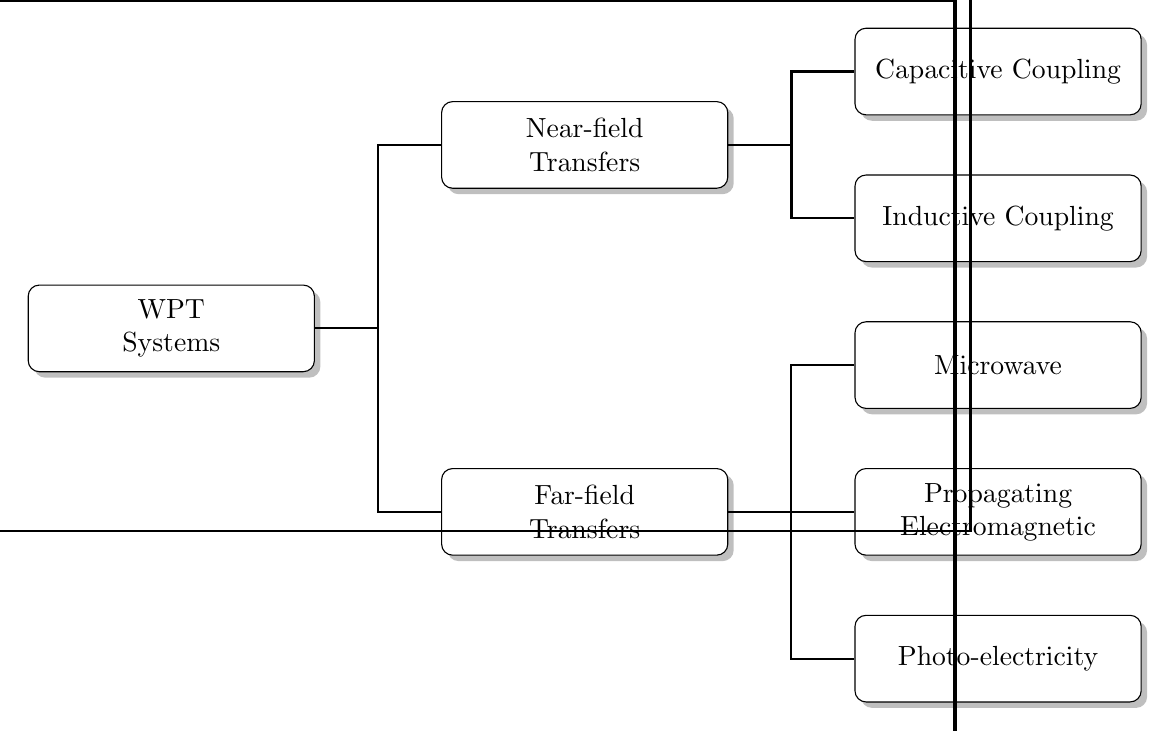
\begin{tikzpicture}[  grow'=right,
                      level distance = 5.25cm,
                      sibling distance = 0.75cm
                    ]

\tikzset{edge from parent/.style = {thick, draw, edge from parent fork right},
         every tree node/.style =
            {rectangle,rounded corners,drop shadow,draw,fill = white,minimum width = 2.8cm, minimum height = 1.1cm,text width = 3.4cm,align = center, text = black}}

\Tree 
    [. {WPT\\ Systems} 
        [.{Near-field\\ Transfers}
            [.{Capacitive Coupling} ]
            [.{Inductive Coupling} ]
        ]
        [.{Far-field\\ Transfers}
            [.{Microwave} ]
            [.{Propagating\\ Electromagnetic} ]
            [.{Photo-electricity} ]
        ] 
    ]

\end{tikzpicture}
\caption{Types of wireless power transfer inside the EM spectrum}
\label{fig:classification}
\end{figure}

%--------------

\section{Discussion}\label{sec:discussion}

% The inductive coupling is the only viable power transfer method which met all the requirements in terms of power and efficiency. It also accomplishes the first and one of the most important proposal in this work, to design a small wireless transfer system capable to be carried in a nano quadcopter.

% Discussion Radiative vs. Non-radiative
In radiative techniques $\vec{E}$ and $\vec{B}$ field strength decreases with distance from the source as $1/r^2$ for the radiated power intensity of electromagnetic radiation. However, near-field $\vec{E}$ and $\vec{B}$ strength decreases more rapidly with distance, being proportional to $1/r^3$. We could think this can be a bother when transferring power. And that is true, but this effect is mostly notable when transmitting over long-distance, which is not the priority of the project. This advantage of far-field over near-field techniques lies on the capability to focus electromagnetic radiation by reflection or refraction into beams. To achieve this narrow beams are necessary antennas much larger than the wavelength of the waves, corresponding to frequencies above 1 GHz, in the microwave range or above. Far-field techniques were rapidly refused because of the physical constraints of the transmitter antenna size, discussed on section \ref{subsec:geo}.

% Discussion between Non-radiative 
Seeing all the available technologies scope inside non-radiative techniques it is quite reasonable to guide towards Resonant Magnetic Induction. This power transfer is reminiscent of the usual magnetic induction; however, the usual non-resonant induction is very inefficient for midrange applications which compromise distances from one antenna diameter up to ten times the antenna diameter \cite{Karalis200834}. % 1e6 más eficiente
As opposed to directed electromagnetic radiation, such as lasers, it does not need an uninterrupted line of sight between the source and the device, as well as a sophisticated tracking mechanism when the device changes its position.

In addition, the fact that magnetic fields interact so weakly with biological organisms is also important for safety considerations \cite{TechTalk}. Capacitive coupling was rejected because of safety issues related to the necessity of a high source voltage. 

To summarize, Resonant Magnetic Induction was the unique WPT system which met mostly all requirements. It allows us to transfer power, nearly omni-directional, over midrange distances in a efficient way. Furthermore, this WPT system is irrespective of the geometry of the surrounding space, with low interference and losses into environmental objects. It also accomplishes the first and one of the most important proposal in this work; to design a small wireless transfer system capable to be carried in a nano-quadcopter.


\begin{table}[ht]
\begin{center}
\begin{tabular}{|l|c|c|c|c|}
% \hline
\rowcolor{black!60}
\hline
\color{white}WPT system                    & \color{white}Frequency   & \color{white}Directivity   & \color{white}Range   & \color{white}Efficiency    \\ \hline %\hline
\rowcolor{gray!54}
Capacitive Coupling           & Low Hz$\sim$MHz     & Weak         & Short       & High             \\ \hline
\rowcolor{white}
Inductive Coupling            & Low Hz$\sim$MHz     & Weak         &  Short      & High             \\ \hline
\rowcolor{gray!40}
Propagating Electromagnetic   & Medium MHz$\sim$GHz       & Medium         &  Medium      & Medium             \\ \hline
\rowcolor{white}
Microwave   & High GHz$\sim$THz       & Strong         &  Long      & Low             \\ \hline
\rowcolor{gray!40}
Photo-electricity   & High $>$THz       & Strong         &  Long      & Low             \\ \hline % Light waves

\end{tabular}
\caption{A comparison among the wireless power transfers}
\label{T:types}
\end{center}
\end{table}

\chapter{Modeling Magnetic Induction System}\label{C:modeling}
A model is probably the most important part when designing a system. Therefore, the system modeling has been studied in detail in order to reproduce reality as close as possible. It is a great advantage to have a reliable model which can reproduce system's behaviour for any conditions. The model will provide us not only with the characterization of the power coils, but also will forecast the operating system constraints.

\section{Magnetic Field}\label{sec:magneticField}
The magnetic field can be produced as consequence of a point charge $q$ moving at a velocity $\vec{v}$ in the space or when a current $I$ is flowing through a length element $d\vec{l}$. The moving point charge $q\vec{v}$ and the current element $Id\vec{l}$ are named sources of the magnetic field.
The most suitable source to determine the magnetic field due to a current loop is an infinitesimal current element. In this case, the expression to compute the magnetic field at a distance $r$ is called Biot-Savart law:
\begin{equation}
d\vec{B} = \frac{\mu_0}{4\pi}\:\frac{I\:d\vec{l}\times{\hat{r}}}{r^2}
\end{equation}

where $\mu_0$ is a constant of proportionality named the magnetic constant (permeability in free space) and has the exact value of $4\pi\cdot{10}^{-7}\:$T$\cdot$m/A.

Imagine that a current flows through a circular loop of radius $R$ made of a conductive material. The magnitude of the magnetic field at a point on the axis of this loop can be determined using the Biot-Savart law. As figure \ref{F:magneticField} shows, the generated magnetic field is perpendicular to $\hat{r}$ and also to $Id\vec{l}$ and follows the expression below:
\begin{equation*}
\lvert d\vec{B} \rvert = \frac{\mu_0}{4\pi}\:\frac{I\:d\vec{l}}{(z^2+R^2)}
\end{equation*}

where in comparison to the Biot-Savart law, $r^2=z^2+R^2$ and the vectorial product $\lvert d\vec{l}\times{\hat{r}}\rvert$ is equal $dl$ because $d\vec{l}$ is perpendicular to $\hat{r}$.

When we sum around all the current elements in the loop, the components of $d\vec{B}$ perpendicular to the axis of the loop sum to zero, which leave only the component $dB_z$ that is parallel to the axis \cite{tipler}. By developing the equation, $dB_z$ can be expressed as:
\\
\begin{equation*}
dB_z=\frac{\mu_0}{4\pi}\:\frac{I\:dl}{(z^2+R^2)}\:sin\theta\:=\:\frac{\mu_0}{4\pi}\:\frac{I\:dl}{(z^2+R^2)}\:\frac{R}{\sqrt{z^2+R^2}}\:=\:\frac{\mu_0}{4\pi}\:\frac{R\:I\:dl}{(z^2+R^2)^{3/2}} \\[10pt]
\end{equation*}

\begin{equation*}
B_z=\oint dB_z=\:\frac{\mu_0}{4\pi}\:\frac{R\:I}{(z^2+R^2)^{3/2}}\oint dl
\end{equation*} \\

In the case of a circular coil, the integral of $dl$ around a loop is $2\pi{R}$ and taking into account that the coil has $N$ turns, the magnetic field on \textit{z} axis can be computed as follows:

\begin{equation}
B_z=\frac{\mu_0}{2}\:\frac{N\:R^2\:I}{(z^2+R^2)^{3/2}}
\label{eq:magneticField}
\end{equation}

\begin{figure}[htb]
\begin{center}
	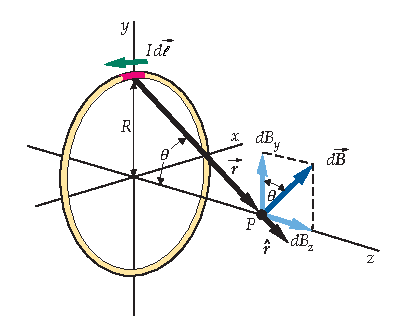
\includegraphics[width=0.55\textwidth]{./images/tip}
\caption{Geometry for calculating the magnetic field at a point on the \textit{z} axis}
\label{F:magneticField}
\end{center}
\end{figure}

	\section{Magnetic Induction}
In the early 1930s Michael Faraday and Joseph Henry independently discovered that in a changing magnetic field a changing magnetic flux through a surface bounded by a closed stationary loop of wire induces a current in the wire \ref{sec:timeline}. This current is also found in a static magnetic field when a changing magnetic flux is created by a moving loop of wire through the surface bounded by the wire itself. 

		\subsection{Magnetic Flux}
The magnetic flux through a surface is the surface integral of the normal component of the magnetic field $\vec{B}$ passing through that surface. In our case these surfaces are defined as the transmitter and receiver coils. As $\vec{B}$ is proportional to the number of field lines per unit area, the magnetic flux is proportional to the number of field lines through an element area \cite{tipler}. Since the coil surface is flat and has a constant area $A$ and several turns $N$, if we assume $\vec{B}$ is uniform in magnitude and direction everywhere on the surface, the magnetic flux through the coil surface is:

  \begin{equation} \label{flux}
    {\phi_m} = \vec{B}\cdot\hat{n}A = NBA\:cos{\theta} 			% Spaces in maths: \,  \:  \;  \!  \(space) \qquad
  \end{equation}

 Where $\theta$ is the angle between the direction of $\vec{B}$ and the direction of the unit vector normal to the coil surface $\hat{n}$.

\begin{figure}[htb]
\begin{center}
	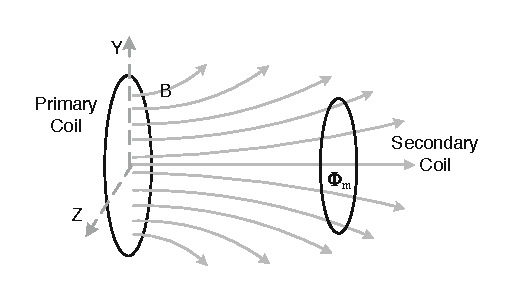
\includegraphics[width=0.7\textwidth]{./images/magneticFlux}
\caption{Magnetic field lines from transmitter to receiver coil}
\label{F:magneticFlux}
\end{center}
\end{figure}

		\subsection{Induced EMF and Faraday's Law}
Equation \ref{flux} shows that flux can be changed by increasing or decreasing $B$, by increasing or decreasing $A$, or by changing the angle ${\theta}$. The idea of changing $A$ or ${\theta}$ is really difficult to achieve and implement compared to changing $B$. Given the magnetic field created by the coil is due to a current in the transmission circuit, the magnitude of the magnetic field can be increased or decreased by increasing or decreasing the current. This change of current will be obtained by using alternating current (AC). The result of this variation of magnetic flux is an emf ${\epsilon}$ induced along the path that is equal in magnitude to the rate of change of the magnetic flux through the surface. This is known as Faraday's law:
  \begin{equation} 
    {\epsilon} = -\frac{d{\theta_m}}{dt}
  \end{equation}

According to the Faraday's law, the polarity of the induced magnetic field is such that it produces a magnetic field opposes the change which produces it. Because the induced voltage and the current are produced at the secondary side, power is successfully transferred from the primary to the secondary side. This is the basic working principles of the inductive coupling.

% begin LLUIS
		\subsection{Inductance}
The simplest way to define what the inductance means is that it is like a resistance but in AC current. It is an opposition to the rate of change of the current. The unit of inductance is the henry (H). As it is shown at follows, one henry is the amount of inductance required to generate one volt when the current is changing at the rate of one ampere per second.
\begin{equation}
{V_L} = L\frac{dI}{dt}
\end{equation}

So it is correct to say that the inductance behaves like a resistance (in AC) because the larger inductance the bigger induced voltage keeping the rate of change of current constant.

In this project are used two types of inductances: the first one, to generate the magnetic flux in one coil, called self-inductance; and the second one, to relate the amount of magnetic flux given by one coil to another coil when they are close enough.

			\subsubsection{Self Inductance}
In this section, the definition of the self-inductance is related to the magnetic field. The reason is because if it is considered a current $I$ going through a coil, this coil generates a magnetic field $B$ that is proportional to $I$\cite{tipler}. The magnetic flux generated by $B$ is also proportional to $I$, as it has expressed in equation \ref{eq:magneticFlux}:
\begin{equation}
\phi_m = L\cdot I
\label{eq:magneticFlux}
\end{equation}

As shown in the previous equation, the inductance $L$ is the proportionality constant and it is called self-inductance. The SI unit of the self-inductance is the henry, as it has said above, and one henry corresponds to one tesla times square meter per ampere.
\begin{equation*}
1\:\textnormal{H} = 1\:\textnormal{T}\cdot\:\textnormal{m}^2/\textnormal{A} = 1\:\textnormal{Wb/A}
\end{equation*}

One possible way to compute the self-inductance of a coil is by calculating, due a knowing current, the magnetic field at every point on the surface bounded by the coil, computing the generated magnetic flux and isolate the self-inductance from the equation \ref{eq:magneticFlux}\cite{tipler}. But the computing of the magnetic field at every point is not a trivial task. Thus, there exist many formulas to easily compute the self-inductance of many types of coils depending on its structure or its geometrical shape, like long solenoids, ferrite-core, air-core and toroid-core inductor, etc. For example, the self-inductance of a long, tightly wound solenoid can be determined by substituting the magnetic flux by the formulas obtained in the electromagnetism theory:
\begin{equation}
\phi_m = NBA = \frac{\mu_0\:N^2\:I\:A}{h}
\end{equation}

where $N$ is the number of turns, and $A$ and $h$ are the coil area and height respectively. If the current flowing through a coil divides the magnetic flux, there is obtained the self-inductance of a long solenoid.
\begin{equation}
L = \frac{\phi_m}{I} = \frac{\mu_0\:N^2\:A}{h}
\end{equation}

These formulas have the characteristic that the value of the coil only depends on the geometrical shape of the coil.
Note that these formulas only depend on the geometrical shape of the coil.

			\subsubsection{Mutual inductance}
Imagine that two or more circuits are close to each other. The amount of magnetic flux through one circuit to the other ones is proportional to the current generated in the first circuit, like the magnetic flux generated by one coil, as we can see in equation \ref{eq:magneticFlux}. The difference is that the proportionality constant is not the self inductance but also is the mutual inductance.

To obtain an expression of the mutual inductance, it is  necessary to know the expression of the magnetic field at a distance $z$. In section \ref{sec:magneticField} it has been determined the equation of computing the magnetic field due to a current loop. This expression can be used for a coil when it is multiplied by $N$ turns. 

Once we have determined the expression of the magnetic field, and considering that two coils are close to each other at a distance $z$, we can obtain an expression of the magnetic flux through the primary coil to the secondary one (equation \ref{flux12}). We will use a similar equation (\ref{flux}) to determine this flux. To simplify the calculations, we are considering that the magnetic flux goes through the perpendicular direction to the area of the primary coil, thus, the value of $cos\:\theta$ becomes one. 

\begin{equation}
\phi_{m12}=M\:I_1\:=\:N_2\:B_1\:A_2
\label{flux12}
\end{equation}

Note that the mutual inductance $M$ is the proportionality constant of the magnetic flux, as it has said above. The equation \ref{eq:magneticField} must be substituted to the equation \ref{flux12} and isolate the mutual inductance.
\begin{equation*}
M=\frac{\mu_0}{2}\:\frac{R_{1}^2\:N_1\:I_1}{(z^2+R_{1}^2)^{3/2}}\:\frac{N_2\:A_2}{I_1}
\end{equation*} \\
\begin{equation}
M=\frac{\mu_0}{2}\:\frac{N_1\:N_2\:R_{1}^2\:R_{2}^2\:\pi}{(z^2+R_{1}^2)^{3/2}}
\end{equation}

As it shows the previous equation, at great distances from the coil, $|z|$ is much greater than $R_1$ and the mutual inductance varies inversely proportional to the distance cubed. This is important to be taken into account because the magnetic flux given by a primary coil to a secondary coil is proportional to the mutual inductance and it will drop rapidly if the distance increases. The conclusion of this is that the closer link distance, the more energy transferred to a secondary coil and a better coupling will be.

	\section{Resonance}\label{sec:resonance}
The resonant circuit, also called LC circuit, can store electrical energy whether it oscillates at its natural frequency (\ref{Eq:naturalFrequency}). The circuit is composed by a coil inductance and a capacitor. The capacitor stores energy in the electric field $E$ between its plates, depending on the voltage across it, and an inductor stores energy in its magnetic field $B$, depending on the current through it. 

		\subsection{Energy Pendulum}
Capacitors and inductors are flip-sides of the same reactive coin, storing and releasing energy in complementary modes. If either the capacitor or inductor starts out in a charged state, by connecting momentarily a battery or by approaching a magnet, the two components will begin to exchange energy between them, back and forth, creating their own AC voltage. 

Frequently, resonance effect is explained using the pendulum analogy comparing the change in kinetic and potential energy to the variation of voltage and current inside the circuit. The pendulum swings at a certain frequency depending on the length of the string holding the mass and not on the mass suspended. In physics, this kind of sine-wave oscillation for a mechanical system is called \textit{Simple Harmonic Motion (SHM)}. The same occurs in the LC circuit where the oscillation and so the frequency are strictly dependent on the sizes of the capacitor and inductor.

\begin{equation}
	\omega_{0} = \sqrt\frac{g}{L}
	\qquad
	\omega_{0} = \frac{1}{\sqrt{LC}}
\label{Eq:naturalFrequency}
\end{equation}

If the power supply frequency for a circuit exactly matches the natural frequency of the circuit's LC combination (Equation \ref{Eq:naturalFrequency}), the circuit is said to be in a state of resonance.

\begin{figure}[ht]
\begin{center}
	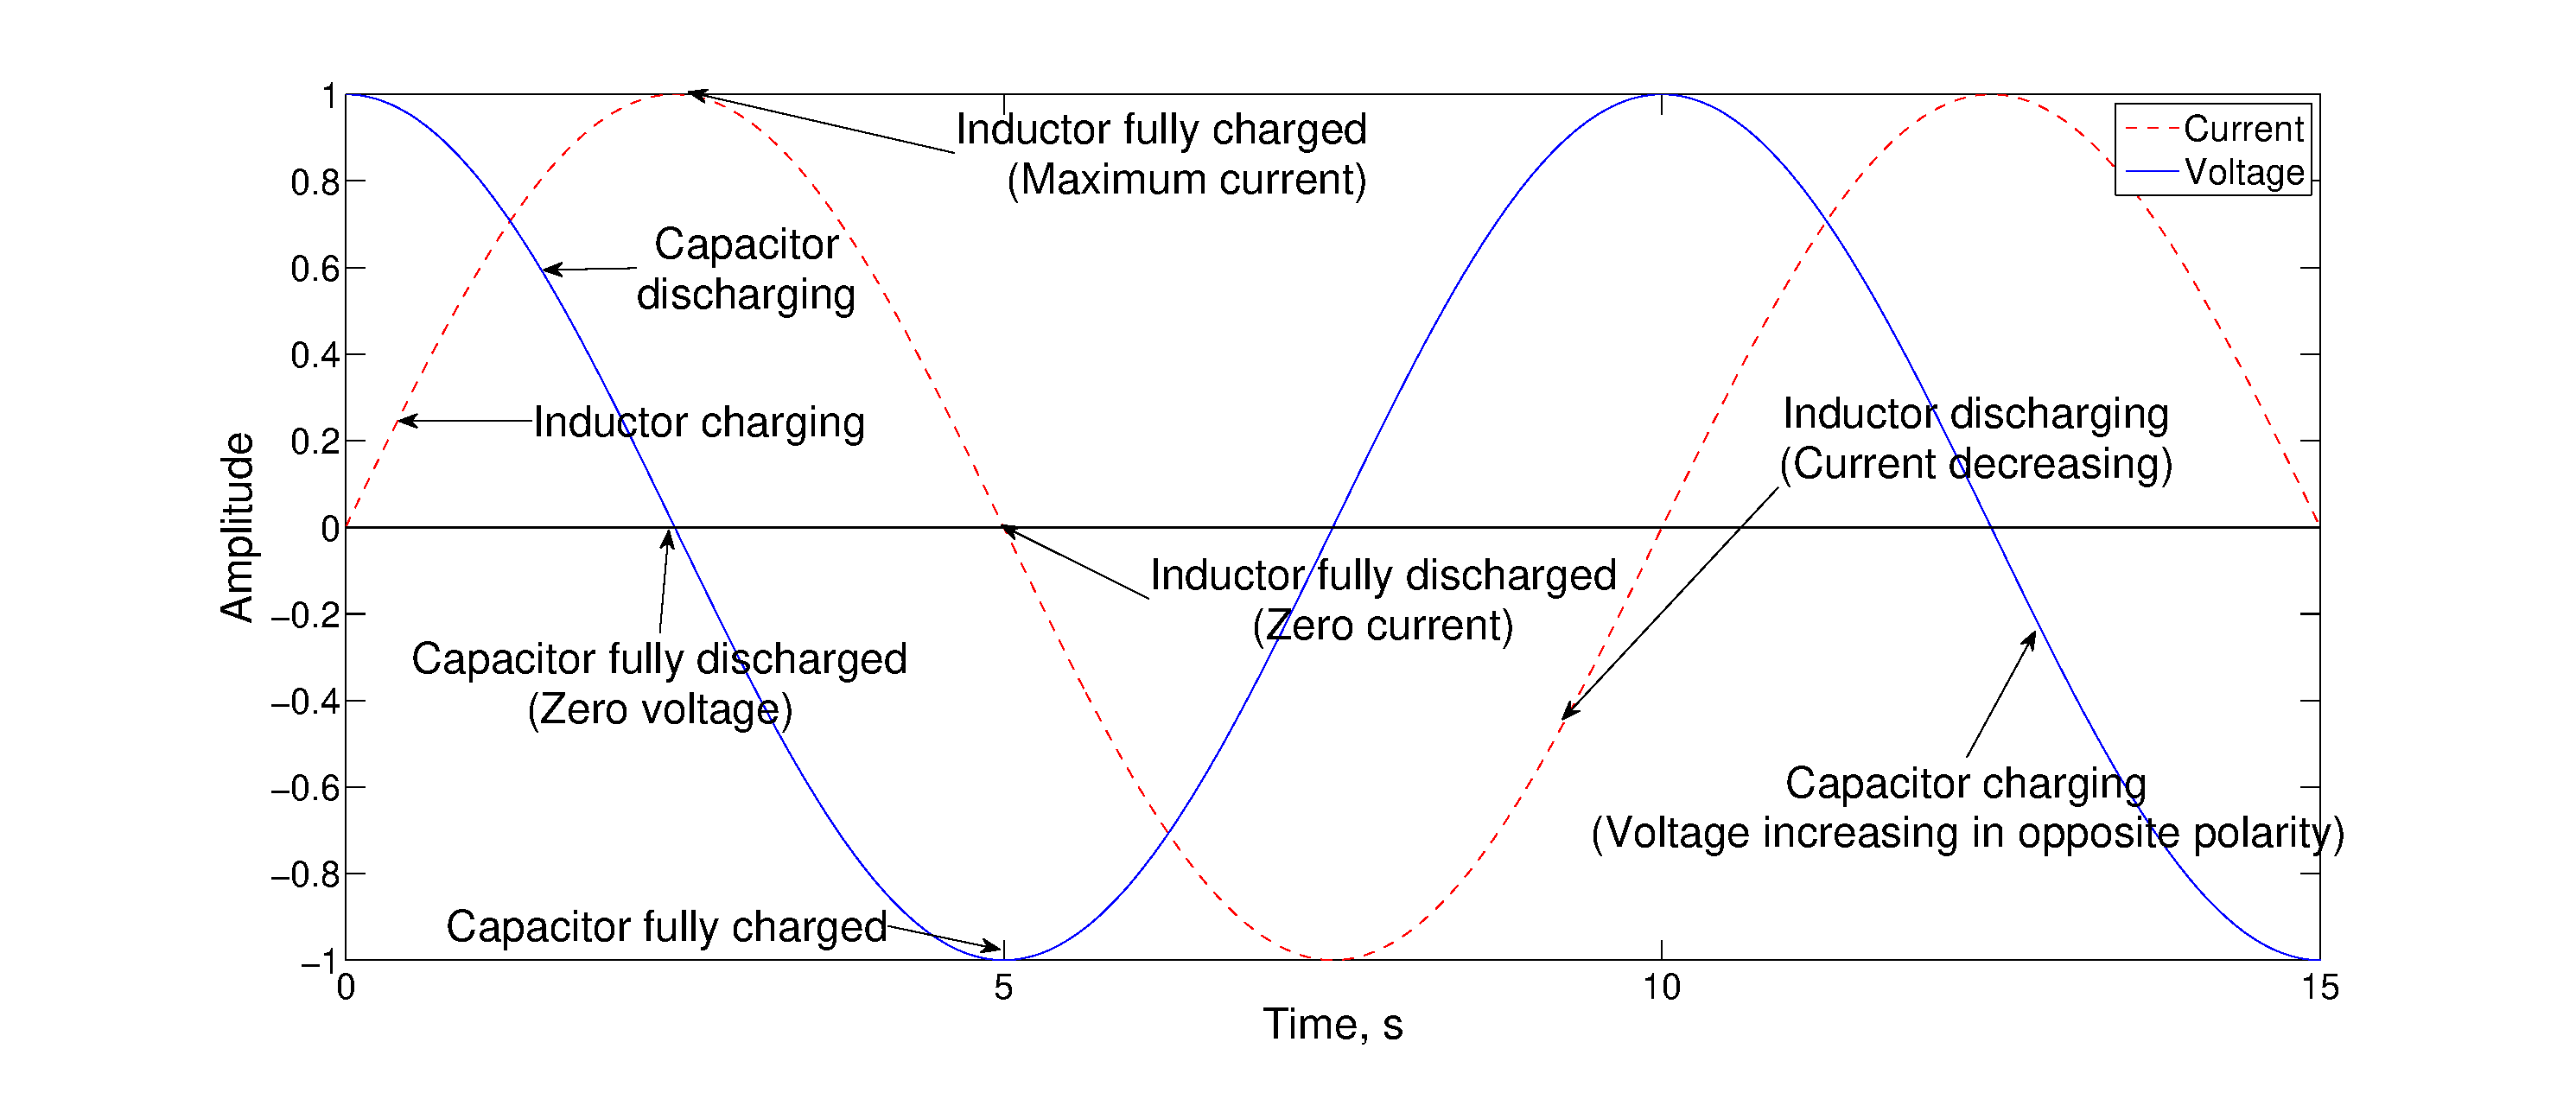
\includegraphics[width=1\textwidth]{./images/VoltageCurrent}
\caption{Voltage and current behaviour inside a LC circuit}
\label{F:VoltageCurrent}
\end{center}
\end{figure}

It can be noticed that there is a phase shift of $90^\circ$ over time between voltage and current measurement in the LC circuit of Figure \ref{F:VoltageCurrent}. This fact will be discussed later. In the same way, whether position and velocity traces of the pendulum were drawn, the same phase shift will be observed.

Both the mechanical and electrical circuits once they have began to oscillate do not last forever. Either resistive or friction losses are the responsible of a finite lifetime.

The pendulum analogy is totally valid for explaining all kind of resonances (e.g., acoustic, mechanical, electromagnetic, etc.) but not enough clear for understanding the resonance between two magnetically coupled resonators. For the purpose of understanding better the behaviour of a coupled system, we think it would be useful to quote the following analogy from F. Hadley\footnote{Franklin Hadley is a Professor with Tenure in the Department of Mechanical Engineering and Materials Science in Duke University.}:

\textit{``Imagine a room with 100 identical wine glasses, each filled with wine up to a different level, so they all have different resonant frequencies. If an opera singer sings a sufficiently loud single note inside the room, a glass of the corresponding frequency might accumulate sufficient energy to even explode, while not influencing the other glasses. In any system of coupled resonators there often exists a so-called `'strongly coupled'` regime of operation. If one ensures to operate in that regime in a given system, the energy transfer can be very efficient.''} 

In our case, the transmitter coil instead of irradiating the environment with electromagnetic waves, it fills the space around it with a non-radiative magnetic field oscillating at a fixed frequency. The non-radiative field mediates the power exchange with the receiver coil, which is specially designed to resonate with the field. The nature of the process ensures a strong interaction between the coils, while minimizing the interaction with the rest of objects \cite{TechTalk}.

The use of resonance results in a much higher efficiency compared to non-resonant inductors, such as typical transformers which require very short range. In addition, by working at the resonant frequency the circuit can achieve its maximum amplitude.

		\subsection{Series Resonance}\label{subsec:seriesResonance}
In order to analyse both series and parallel resonance, a resistance has been added to avoid infinity currents and zero voltage values. These RLC circuits will provide a first approach for understanding the differences when designing the resonant circuit. 

As it is said before, resonance occurs when a series resonant circuit is driven from an external source at a frequency $\omega_0$ at which the inductive and capacitive reactances are equal in magnitude. 

\begin{equation*}
	X_L = X_C
\end{equation*}

This cancellation leaves only the resistance\footnote{An LC circuit is an idealized model since it assumes there is no dissipation of energy due to resistance.} to contribute to the impedance,

\begin{equation*}
	Z_{min} = \sqrt{R^2+(X_L-X_C)^2} = R
\end{equation*}

The impedance is also at a minimum at resonance (see Figure \ref{F:series1}). Below that natural frequency, called resonant frequency $\omega_{res}$, the series resonant circuit looks capacitive since the impedance of the capacitor increases while inductive reactance is decreasing. Above resonance the circuit behaves oppositely.

\begin{figure}[h!]
  \begin{center}
    \begin{circuitikz}
    \ctikzset{v/.append style={/tikz/american voltages}}
    \ctikzset{bipoles/resistor/height=0.25}
    \ctikzset{bipoles/resistor/width=0.7}
      \draw (0,0)
      to[sinusoidal voltage source,v=$V_{S}$] (0,3)
      to[short] (1,3)
      to[C=$C$] (2,3)
      to[short] (3,3)
      to[L=$L$] (4,3)
      to[short] (5,3)
      to[R=$R$,v_=$V_R$,-] (5,0)
      to[short] (0,0);

    \end{circuitikz}
    \caption{Series resonance}
  \end{center}
\end{figure}

At resonance frequency, due to the smallest circuit impedance, the current is greatest, 

\begin{equation}
	I_{max} = \frac{V}{Z_{min}}
\end{equation}

Thus, resonant current peak is set by the resistor value.

\begin{figure}[htb]
\begin{center}
\begin{subfigmatrix}{2} 
\subfigure[Impedance and reactance w.r.t. frequency] % With Respect To
	{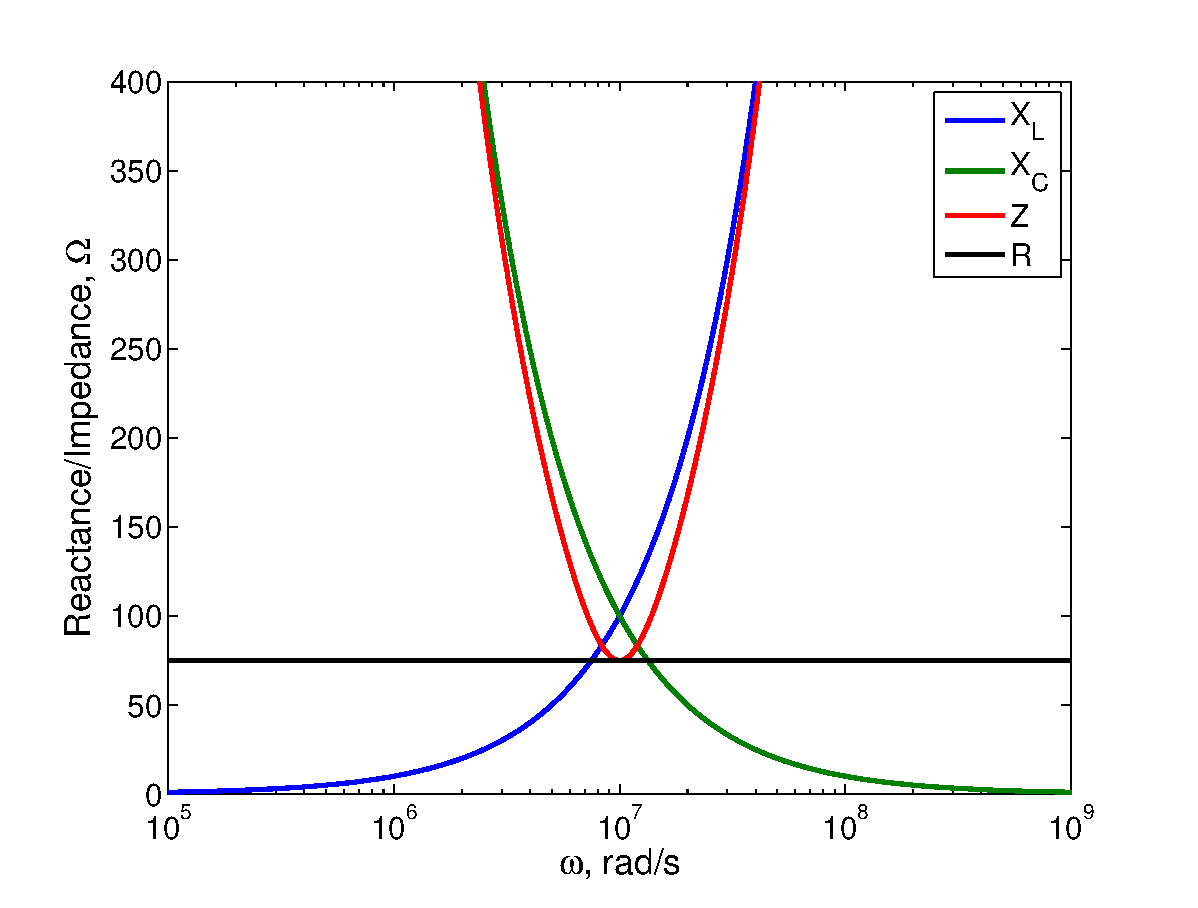
\includegraphics{./images/series1}\label{F:series1}} 
\subfigure[Voltage gain in the resistor]
	{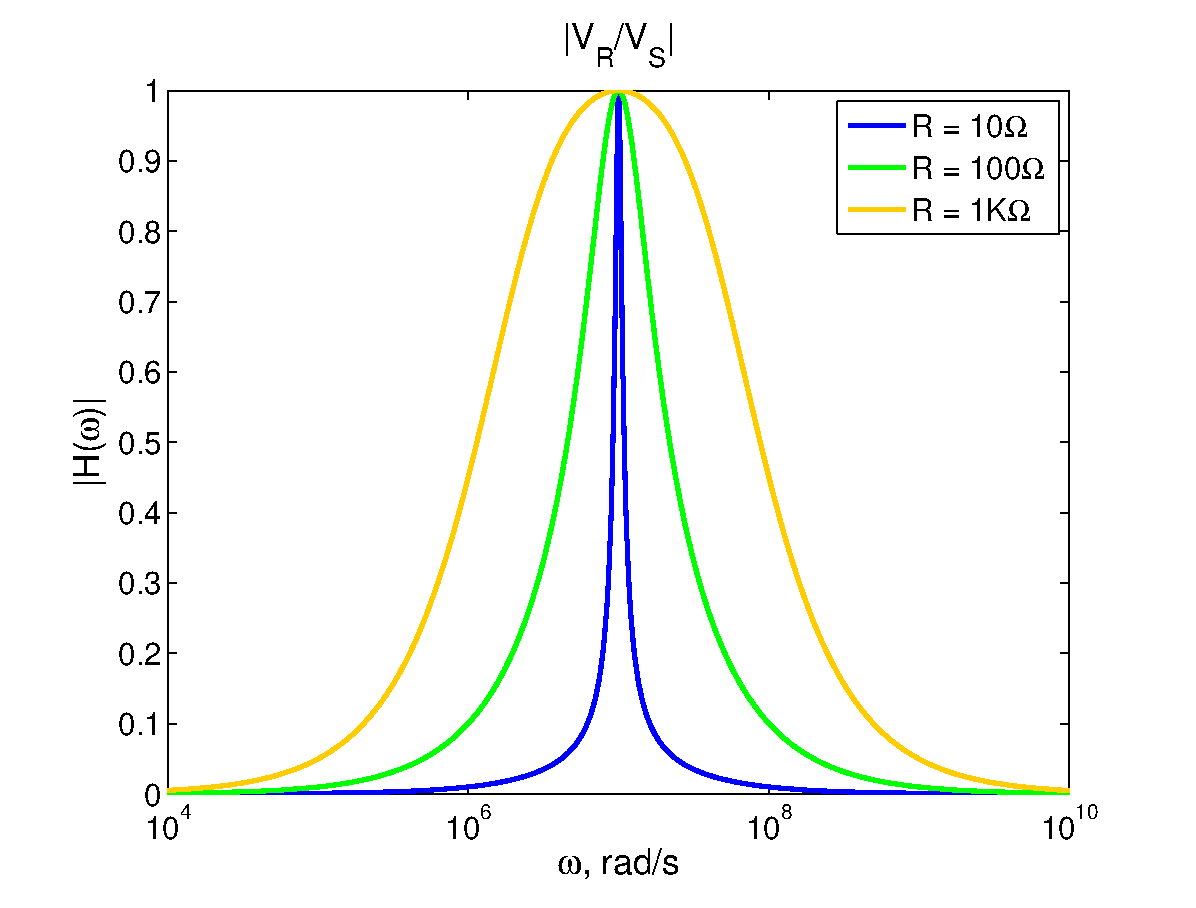
\includegraphics{./images/series2}\label{F:series2}}
\end{subfigmatrix}
\caption{Series RLC circuit}
\label{F:seriesRLC}
\end{center}
\end{figure}

		\subsection{Parallel Resonance}
In the same way as series resonance, the parallel resonant circuit is purely resistive at $\omega_{res}$, where $X_L = X_C$. 


\begin{figure}[hbt]
  \begin{center}
    \begin{circuitikz}
    \ctikzset{v/.append style={/tikz/american voltages}}
    \ctikzset{bipoles/resistor/height=0.25}
    \ctikzset{bipoles/resistor/width=0.7}
      \draw (0,0)
      to[sinusoidal voltage source,v=$V_{S}$,i^=$i_S$] (0,3)      
      to[short] (3,3)
      to[C=$C$] (3,0)
      to[short] (0,0);
      \draw (3,3)
      to[short] (5,3)
      to[L=$L$] (5,0)
      to[short] (3,0);
      \draw (5,3)
      to[short,i=$i_R$] (7,3)
      % to[short,i=$i_R$] (7,2)
      to[R=$R$] (7,0)
      to[short] (5,0);
    \end{circuitikz}
    \caption{Parallel resonance}
  \end{center}
\end{figure}

This time the parallel RLC circuit has a current gain rather than a voltage gain. Its impedance is maximized at the resonant frequency rather than minimized.

Below this frequency, the resonant circuit looks inductive since the impedance of the inductor is lower. Above resonance, the capacitive reactance decreases. In both cases the current drawn is larger than the current at resonance case \cite{aacResonance}. In both parallel and series circuits, the resonant frequency remains the same.

\begin{figure}[htb]
\begin{center}
\begin{subfigmatrix}{2} 
\subfigure[Impedance and reactance w.r.t. frequency] % With Respect To
	{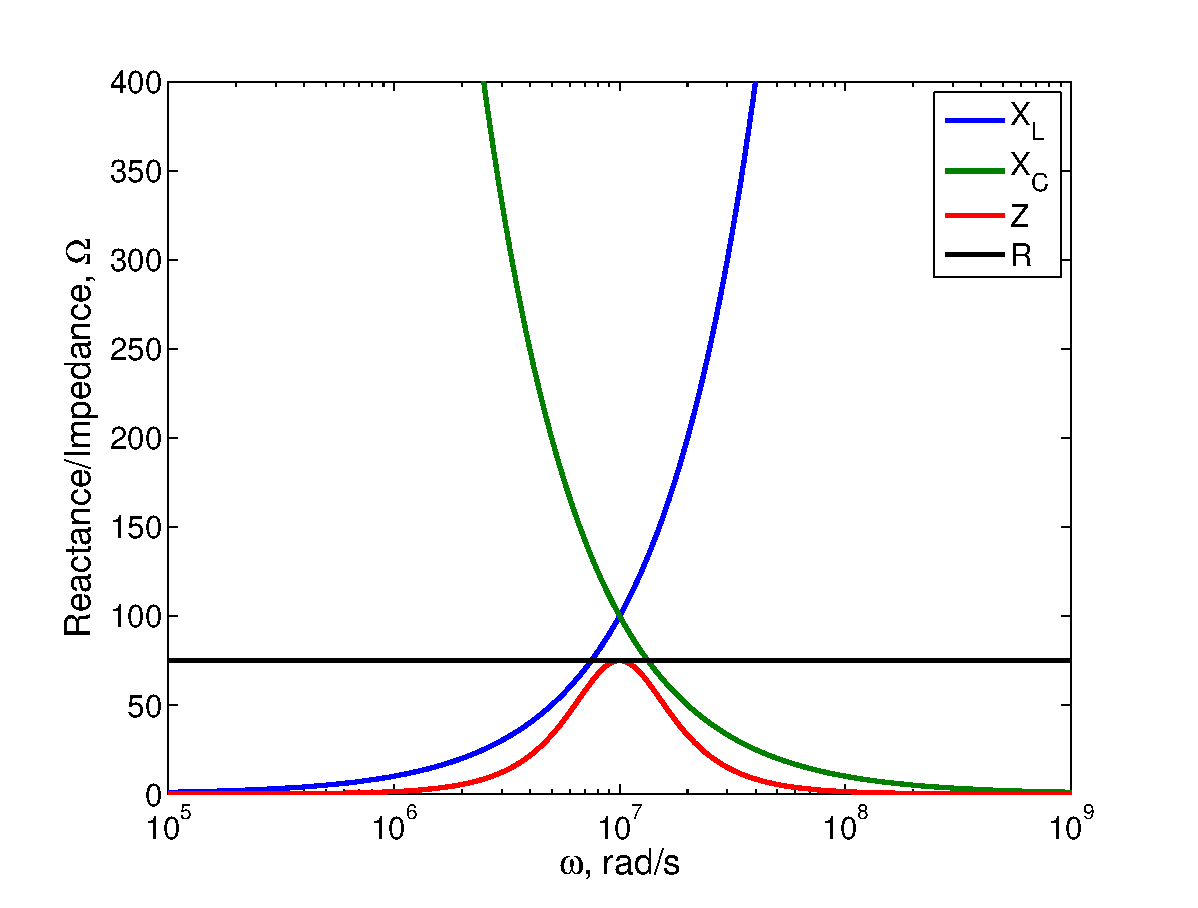
\includegraphics{./images/parallel1}\label{F:parallel1}} 
\subfigure[Current gain in the resistor]
	{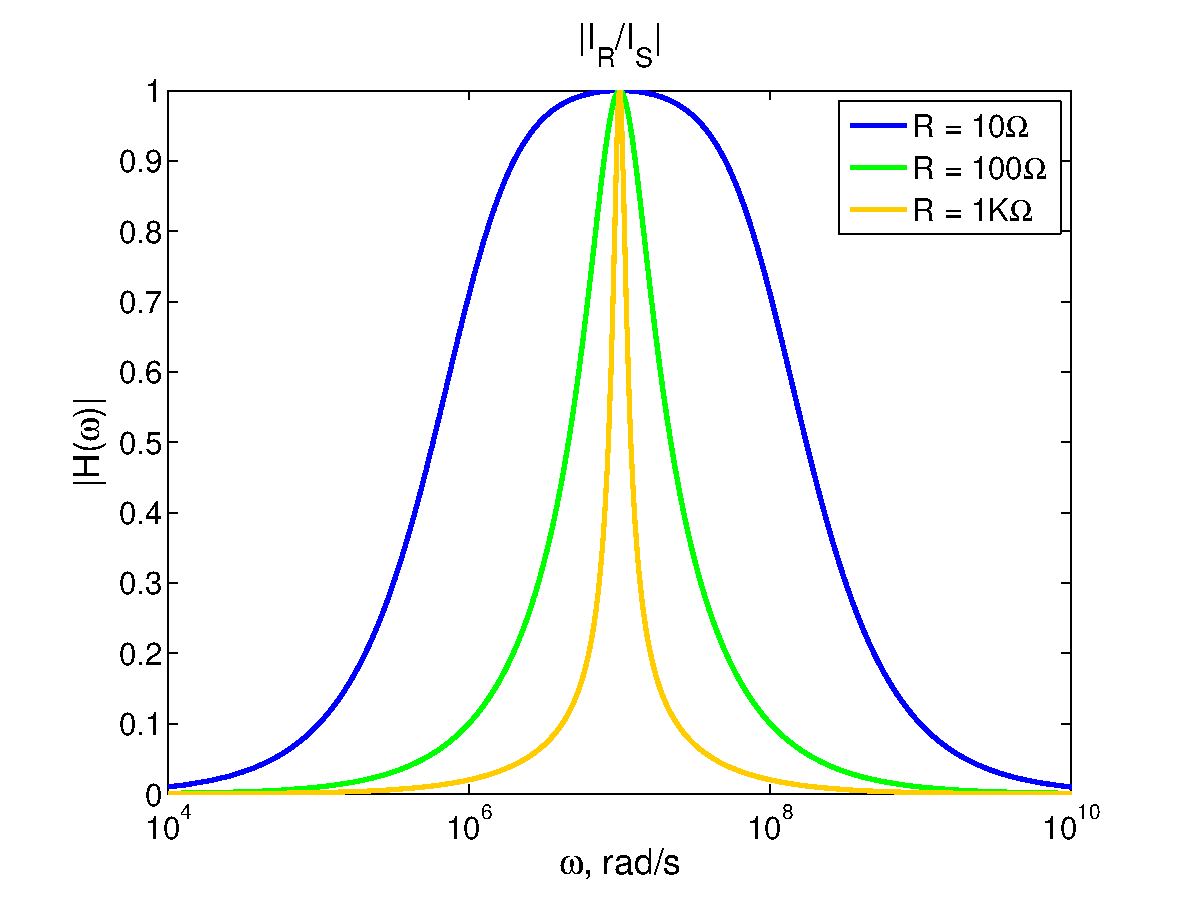
\includegraphics{./images/parallel2}\label{F:parallel2}}
\end{subfigmatrix}
\caption{Parallel RLC circuit}
\label{F:parallelRLC}
\end{center}
\end{figure}

Figure \ref{F:parallel1} shows how impedance is at a peak at resonant frequency and therefore voltage is maximum. The reason for this is that voltage is proportional to impedance. 

\begin{equation}
	V = I\cdot{Z}
\end{equation}

 % This is satisfactory if the resistances are small (http://hyperphysics.phy-astr.gsu.edu/hbase/electric/parres.html)

	\section{Characterizing the Inductor} %Coil Modeling
In order to transfer power wirelessly, the LC-pair is adopted because it is the oldest and most frequently used technique. It is rapidly assembled by winding a \textit{piece} of wire and placing a capacitor either in series or parallel, depending on the desire effect. The capacitor is adopted at both side to keep the coils resonate at the designed frequency.

There are many ways to model a coil. Figure \ref{F:modelingCoil} shows one of them, composed by the coil inductance $L$ itself and a coil conductor resistor $R$. This resistance is placed to quantify \textit{Copper loss} or winding loss which is the term used to describe the energy dissipated by resistance in the wire used to wind the coil \cite{CopperLoss}. There is also an equivalent parasitic capacitor $C_{p}$ connected to the inductor and resistor. This parasitic capacitance is due to the fact that the inductor is made out of a coil of insulated wire. Therefore, tiny capacitors are created between the windings since there are two sections of wire separated by an insulator. 

Another simplified equivalent circuit is shown on the right in Figure \ref{F:modelingCoil}. The impedance of the coil is represented by a real impedance component $Re$ and an imaginary impedance component $Im$ (impedance equations are presented in Appendix \ref{AppendixSection: impedance}). This modeling approach has been verified, especially in the low frequency range\cite{medical}. For high-accuracy applications, like PCB spiral coils, complex models \cite{Eddy} can be used. 

\begin{figure}[h]
\begin{center}
	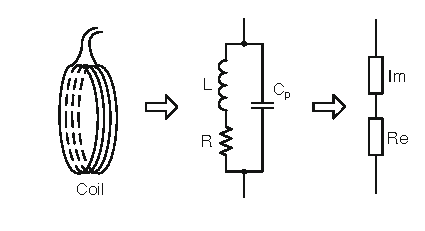
\includegraphics[width=0.7\textwidth]{./images/med}
\caption{Modeling of a single magnetic coil}
\label{F:modelingCoil}
\end{center}
\end{figure}

		\subsection{Coil Resistance}\label{subsec:coilResistance}
The calculation of the resistance of a coil is important because it limits the power transferred in a WPT system. If the resistances of a coil were zero, the power transfer efficiency would be 100$\%$, and there would not exist any limitation to transfer energy at a given distance. However, the ideal world does not exist and appear resistances that generate heat due to Joule effect: power losses. The goal of a WPT system is to minimize this power losses to ensure the maximum transferred power and efficiency.

\subsubsection{DC Resistance}
At low frequencies ($f<$ 200 kHz) \cite{meyer} the resistance experiments a DC behavior. The value of this resistance does only depend on the wire geometry and material. The DC resistance of a metal conductor is given by \cite{medical}

\begin{equation}
R_{DC}=\rho\:\frac{l}{S}
\label{DCres}
\end{equation}

where $l$ is the wire length in meters, $S$ is the wire section in square meters and $\rho$ is the electrical resistivity of the metal material, measured in $\Omega\cdot$m. In table \ref{T:electricalResistivity} are exposed different electrical resistivities for some metal conductors.

\subsubsection{AC Resistance}
When the frequency increases up to 200 kHz we can not talk anymore about DC resistance, the reason is the appearance of some effects that increase the wire resistance with the frequency. From now on, the resistance will behave as an AC resistance due to the \textit{skin-effect} and \textit{proximity-effect}. 

\textit{Skin-effect} happens in all wire and cable. When the signal is DC, it uses the entire conductor, with the same amount of current flowing in the center of the wire as on the outside. As the frequency is increased, the current density begins to move further away from the conductor that inside it. Consequently, the equivalent cross section of the conductor decreases and as Figure \ref{F:skinDepth} shows, the wire resistance is increased with frequency. To quantify the \textit{skin-effect} it is introduced the skin depth $\delta$. Skin depth is a measure of how far electrical conduction takes place in a conductor, and is a function of frequency, no matter how thick the wire is. It is calculated as described below \cite{mit2},


\begin{equation}
% \delta=\sqrt{\frac{2\:\rho}{\omega\:\mu}}
\delta = \frac{1}{\sqrt{\pi{f}\mu\:\sigma}}
\end{equation}

where $\sigma$ is the electrical conductivity of the wire material ($\sigma_{copper}=5.8 \text{ x } 10^7$ S/m), $f$ is frequency in Hz and $\mu$ is the total permeability defined as the permeability in free space times the material permeability ($\mu=\mu_0\cdot{\mu_m}$). 

Owing to skin depth decreases with respect to the frequency as a negative exponential, conductors can become thinner at higher frequencies with little impact on circuit loss, because skin depth shrinks with frequency. A rule of thumb is always plan on providing at least five skin depths of low-loss conductor in order to provide good performance without the need of invest better conductors \cite{skinDepth}. This effect can be reduced by using \textit{Litz wire} \cite{ACres}.

The resistance corresponding to  \textit{skin-effect} can be determined in the following way:

\begin{equation}
R_{skin}=R_{DC}\:\frac{4\:d}{\delta}
\end{equation}

The $R_{skin}$ is the result of multiplying the $R_{DC}$ by the coefficient $4d/\delta$, which is proportional to the square root of the frequency.

\begin{figure}[htb]
\begin{center}
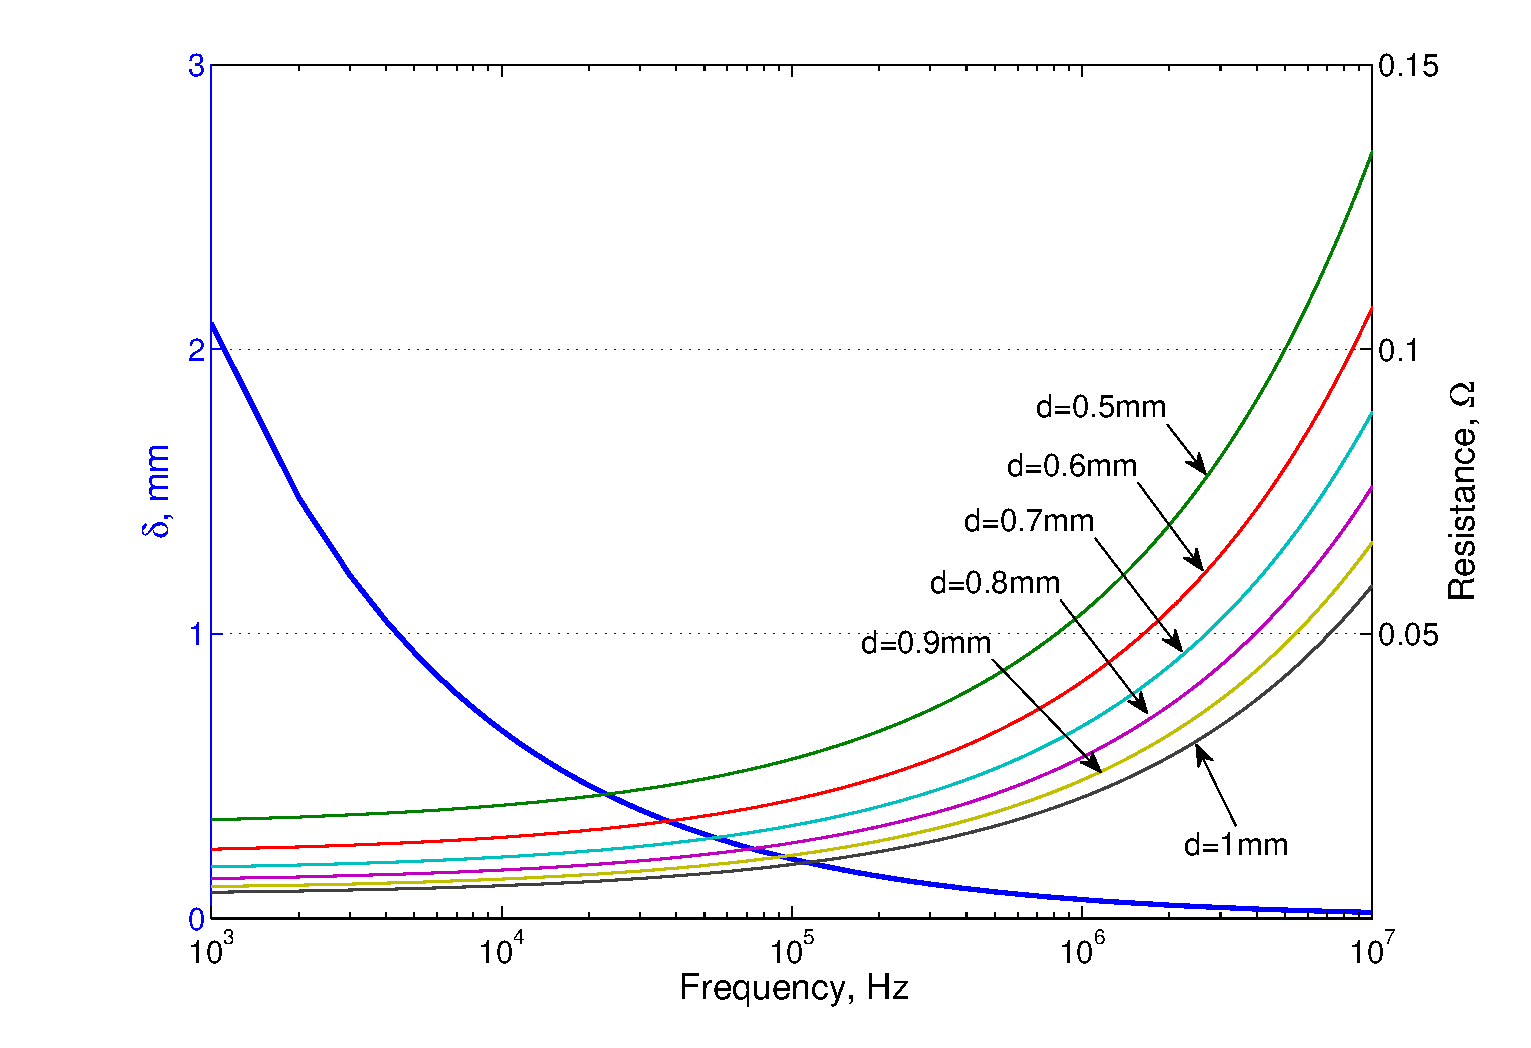
\includegraphics[width=0.7\textwidth]{./images/skinDepth}
\caption{Skin depth and resistance varying frequency for a fixed coil}
\label{F:skinDepth}
\end{center}
\end{figure}

Besides the \textit{skin-effect} there is another phenomena that increase the resistance value of a conductor when is applied an alternating current, called \textit{proximity-effect}. This effect is the apparent increase in the resistance of the wire due to the circulating current in the conductor caused by the alternating flux of the other nearby conductors. As a result, more power losses in the windings appear. To quantify the \textit{proximity-effect}, there is used the Dowell's assumption \cite{ACres}:
\begin{equation}
R_{proximity} = R_{DC}\:\psi\:\left [ \frac{sinh(2\:\psi)+sin(2\:\psi)}{cosh(2\:\psi)-cos(2\:\psi)}+\frac{2}{3}(m^2-1)\frac{sinh(2\:\psi)-sin(2\:\psi)}{cosh(2\:\psi)+cos(2\:\psi)} \right ]
\end{equation} 

In the above equation, the parameter $\psi$ can be determined in the following form:
\begin{equation*}
\psi = \left ( \frac{100\:d}{2\:\delta} \right )\:\sqrt{\pi}
\end{equation*}

Here, $m$ indicates the number of layers, and $\delta$ is the skin depth previously mentioned.

To conclude this section, the total equivalent series resistance $R_{ES}$ that appears when an alternating current flows through a wire is the sum of all these effects in addition to the ``parasitic'' resistance of the wire, called DC resistance. 

\begin{equation}\label{eq:Resistance}
R_{ES} = R_{DC}+R_{skin}+R_{proximity}
\end{equation} 
%%%%%%%%%%%%%%%%%%%%%%%%%
% Resistencia radiación %
%%%%%%%%%%%%%%%%%%%%%%%%%

		\subsection{Coil Inductance}\label{subsec:coilInductance}
In this project air-core inductors are required due their low weight compared to solid-core, despite the last provide better coupling. The reason of avoiding better \textit{transformers}, as it said in previous sections, is that the primary coil is wanted to go on a nano-quadcopter. Thus, the most typical formulas to compute the self-inductance of an air-core inductor are exposed below.

The most typical formula that is used in many projects or studies is the equation of a circular loop coil \cite{TypicalL},\cite{UAV},\cite{Melliptical}:

\begin{equation}\label{Eq:typical}
L=\mu_0\:R\:N^2\:(ln\frac{8R}{d/2}-1.75)\qquad [\textnormal{H}]
\end{equation}

where $d$ is the wire diameter.

Another equation is the Harold A. Wheeler’s formula to compute the inductance for a finite-length solenoid:
\begin{equation}\label{Eq:Harold}
L=\frac{N^2\:R^2}{9R+10h}\qquad [\mu \textnormal{H}]
\end{equation}

The units of length are expressed in inches. This formula is correct to within 1 per cent for coils with $h>0.8R$ \cite{wheeler}.

Similar to the Harold A. Wheeler’s formula, an equation for air-cored inductor is exposed below \cite{WaiKaiChen}:
\begin{equation}\label{Eq:Wai}
L=2\:K\:R\:N^2\qquad [\mu \textnormal{H}]
\end{equation}

where $K$ is a parameter that depends on the dimension ratio ($D/h$) of the coil, whose values are listed in Appendix \ref{Appendix: AA} and the units of length in this equation are expressed in centimeters.












		\subsection{Coil Parasitic Capacitor}
Every coil has a parasitic capacitor. Since the inductor is made out of a coil of insulated wire, tiny capacitors between the windings are created. This is due each section of windings is at a slightly different potential because of wire inductance and resistance. When the current frequency is high enough, most current in the coil would be bypassed via the parasitic capacitor \cite{medical}. As a result, the coil can not be viewed as a lumped inductor anymore. The coil's inductance would resonate with the parasitic capacitor at a frequency. This frequency is called the self-resonant frequency ($f_s$).

\begin{equation}
	f_{s} = \frac{1}{2\pi\sqrt{LC_{par}}}
\end{equation}

The parasitic capacitance is connected in parallel to the inductor and the resistor. Its value is relatively small, of the order of 1 pF, which is insignificant at low frequencies but not at very high frequencies ($>$ 5 MHz) \cite{tesis}. Because of this capacitance, the coil has a self-resonance frequency between 10 MHz and 25 MHz.

The parasitic capacitance effect can be alleviated by keeping inductor windings far apart, and so reducing the capacitance by using helical coils. The second option to reduce parasitic capacitors is to work at a frequency low enough. This frequency will be discussed in Section \ref{subsec:operatingFreq}. For the following theorical model parasitic capacitors will be disregarded.

	\section{Coreless Transformer Modeling}
In this section the electrical model of the resonant magnetic induction system will be determined by using the air coreless transformers theory, in which WPT systems are based on. It is called transformer because it transforms electrical energy into magnetic energy, then back into electrical energy again. Because its operation depends on electromagnetic induction between two stationary coils and a magnetic flux and polarity, transformers are necessarily AC devices. 














\begin{table}[h]
\begin{center}
\begin{tabular}{|c|c|}

\noalign{\global\arrayrulewidth1pt}
\hline
\textbf{Parameter} 	& 	\textbf{Definition}\\
\hline
\hline
$V_S$ 		& Source voltage		\\ \hline 
$I_1$  		& Primary current		\\ \hline 
$I_2$  		& Secondary current		\\ \hline 
$R_1$  		& Primary resistance	\\ \hline 
$R_2$ 		& Secondary resistance	\\ \hline 
$R_L$		& Load resistance		\\ \hline
$L_1$		& Primary inductance 	\\ \hline
$L_2$		& Secondary inductance 	\\ \hline
$C_1$		& Primary capacitor 	\\ \hline
$C_2$		& Secondary capacitor 	\\ \hline
$M$			& Mutual inductance 	\\ \hline
$\omega$	& Angular frequency 	\\ \hline     
\end{tabular}
\caption{Electric parameters}
\label{T:Electric parameters}
\end{center}
\end{table}

% Its working principle consists in appliying a high frequency current in the transmitter coil. Hence, only a percentage of the alternating magnetic flux created will penetrate the receiver coil. Thus, a voltage is induced in the receiver side due to magnetic induction.      

		\subsection{Electrical Circuit} \label{subsec:Model}
In the first analysis, the  electric system of non-resonant induction is discussed in a generic way. A typical inductive system consists of a primary transmitter coil (\textit{Tx}) and a secondary receiver coil (\textit{Rx}), but there can be added more coils to the system.

The \textit{Tx} coil is characterized by a winding that has a resistance $R_1$ and an inductance $L_1$. Similarly, the secondary coil \textit{Rx} is characterized by a winding resistance, $R_2$ and an inductance, $L_2$.

\begin{figure}[ht!]
  \begin{center}
    \begin{circuitikz}
    \ctikzset{bipoles/resistor/height=0.25}
    \ctikzset{bipoles/resistor/width=0.7}
     \draw (0,0)
     to[sinusoidal voltage source,v=$V_S$] (0,4) 
	 to[short] (1,4) 
	 to[R=$R_1$] (2,4) 
	 to[short] (3,4)
     to[L=$L_1$] (4,4)
     to[short] (5,4);
     \draw (0,0) 
     to[short] (5,0)
     to[sinusoidal voltage source,v=$jwMI_2$] (5,4);
     \draw (6,0) 
     to[sinusoidal voltage source,v_=$jwMI_1$] (6,4)
     to[short] (7,4)
     to[L=$L_2$] (8,4)
     to[short] (9,4)
     to[R=$R_2$] (10,4)
     to[short] (11,4)
     to[generic=$R_L$] (11,0)
     to[short] (6,0);
      \draw[thin, <-, >=triangle 45] (2,2)node{$i_1$}  ++(-60:0.8) arc (-60:170:0.8);
      \draw[thin, <-, >=triangle 45] (9,2)node{$i_2$}  ++(-60:0.8) arc (-60:170:0.8);
    \end{circuitikz}
   \caption{General electric circuit}
\label{F:Electric}
  \end{center}
\end{figure}
As it can be seen in Figure \ref{F:Electric}, the system does not include compensation capacitors neither in the transmission side nor the reception. Thus, a non-resonant\footnote{Note this is stated for ideal coils which need of a compensation to become resonant.} is studied on a first approach. The system is excited by a perfect sine wave in steady state condition. For simplicity, the lumped element model is assumed regarding that $\lambda$ is much bigger than the characteristic length of the circuit. This assumption declares that all circuit elements, such as resistors, inductors and capacitors, are concentrated into idealized electrical components.

The circuit model offers a convenient way to systematically analyze the characteristic of the system \cite{matrix}. By applying circuit theory Kirchhoff's Voltage Law (KVL) to this system a relationship between currents through each coil and the voltage applied to the transmitter coil can be described as the following equation system:

\begin{numcases}{}
	V_S=R_1\cdot{I_1}+j\omega{L_1}\cdot{I_1}-j\omega{M}\cdot{I_2} \label{eq1}
\\
	0 = R_2\cdot{I_2}+R_L\cdot{I_2}+j\omega{L_2}\cdot{I_2}-j\omega{M}\cdot{I_1} \label{eq2}
\end{numcases}

These equations show how the primary side induces voltage into the secondary side which depends on the frequency, mutual inductance and the primary coil's current, which is also called magnetizing current since it is the responsible of generating the magnetic field and so the magnetic flux.

The system of linear equations can be arranged as the following symmetric matrix \ref{M:kvl}.  

\begin{equation}
\begin{bmatrix}
    V_{S} 	\\
    0 		\\
\end{bmatrix}
=
\begin{bmatrix}
    Z_{1} 			& -j{\omega}M  	\\
    -j{\omega}M 	& Z_{2}  		\\
\end{bmatrix}
\begin{bmatrix}
    I_{1}	\\
    I_{2}	\\

\end{bmatrix}
\label{M:kvl}
\end{equation}

In order to transfer the maximum power and reduce losses the proposed model is based on \cite{meyer}, which defines an equivalent impedance matching method. The procedure analyses the effect of the complete secondary circuit on the primary side. Thus, the secondary circuit is viewed from the voltage supply as a reflected impedance $Z_R$.

Firstly, the secondary current will be isolated from the Equation \ref{eq2}, becoming:

\begin{equation}
	I_2 = \frac{j\omega{M}}{R_2+R_L+j\omega{L_2}}\cdot{I_1}
\end{equation}

To determine the expression of $Z_R$, all the secondary-side components, including the load resistance $R_L$, can be gathered into a single impedance expresion called secondary impedance $Z_2$:

\begin{equation}
	Z_2 = R_2+R_L+j\omega{L_2}
\end{equation}

In the same way, the primary circuit impedance is defined in the next manner:

\begin{equation}
	Z_1 = R_1+j\omega{L_1}
\end{equation}

Now, the current at secondary circuit can be expressed as:

\begin{equation} \label{eq:I2}
	I_2 = \frac{j\omega{M}}{Z_2}\cdot{I_1}
\end{equation}

Substituting $I_2$ in Equation \ref{eq2}, we are forcing voltage source to ``see'' secondary circuit as a single impedance, $Z_R$.

\begin{equation} \label{Eq:ZR}
	V_S = Z_1\cdot{I_1}+\frac{\omega^2{M^2}}{Z_2}\cdot{I_1} 
\end{equation}

where $Z_R$ is defined as:

\begin{equation}
	Z_R = \frac{\omega^2M^2}{Z_2}
\end{equation}

Thereby, equation \ref{Eq:ZR} is rearranged in the form:

\begin{equation}
	V_S =(Z_1+Z_R)\cdot{I_1}
\end{equation}

To simplify even more the expression, it is possible to define the whole circuit as the following single impedance (see Figure \ref{F:equivalentCircuit}):

\begin{equation}
	V_S = Z_{eq}\cdot{I_1}
\end{equation}


\begin{figure}[ht!]
  \begin{center}
    \begin{circuitikz}
	\ctikzset{v/.append style={/tikz/american voltages}}
    \ctikzset{bipoles/resistor/height=0.25}
    \ctikzset{bipoles/resistor/width=0.5}
     \draw (0,0) 
     to[sV,v=$V_S$] (0,4) 
	 to[short] (1,4) 
	 to[R=$R_1$] (2,4) 
	 to[short] (3,4)
     to[L=$L_1$] (4,4)
     to[short] (5,4);
     \draw (5,0) 
     to[generic=$Z_R$] (5,4);
	\draw(5,0)
	to[short] (0,0);
     % to[short] (0,5);
     \draw(5,3) node[anchor=west] {+};
	 \draw (5,1) node[anchor=west] {-};
	 \node at (5.75,2) {$V_{out}$};
    \end{circuitikz}
   \caption{Reflected impedance circuit schematic}
\label{F:reflectedCircuit}  
\end{center}

\end{figure}

\begin{figure}[ht!]
  \begin{center}
    \begin{circuitikz}
	\ctikzset{v/.append style={/tikz/american voltages}}
    \ctikzset{bipoles/resistor/height=0.25}
    \ctikzset{bipoles/resistor/width=0.5}
	\draw (0,0) 
     to[sinusoidal voltage source,v=$V_S$] (0,4) 
	 to[short] (5,4);
     \draw (0,0)
     to[short] (5,0)
     to[generic=$Z_{eq}$] (5,4);
	\draw(5,3) node[anchor=west] { };
	 \draw (5,1) node[anchor=west] { };
	 \node at (5.75,2) {$\qquad$};
    \end{circuitikz}
   \caption{Equivalent impedance circuit schematic}
\label{F:equivalentCircuit}  
\end{center}

\end{figure}

Once the $Z_R$ is determined, it is possible to calculate the voltage drop across it by using the voltage divider expression:

\begin{equation}
	V_{out} = V_S\cdot\frac{Z_R}{Z_R+Z_1}
	\label{eq:vout}
\end{equation}

Hence, the power transferred to the reflected impedance is given by:

\begin{equation}
	P_{out} = \frac{V_{out}^2}{Z_{R}}
\end{equation}

Replacing $V_{out}$ for the expression \ref{eq:vout}, the power at the reflected impedance only depends on the source voltage (also called $V_{in}$).

\begin{equation}
	P_{out} = V_{in}^2\cdot\frac{Z_R}{(Z_1+Z_R)^2}
\end{equation}

For the fixed value of $Z_1$, it is found the optimal $Z_R$ value computing the partial derivative of $P_{out}$ with respect to $Z_L$.
\begin{equation}
	P_{out_{max}}\Rightarrow\frac{dP_{out}}{dZ_R}=\frac{(Z_1+Z_R)^2-2\cdot{Z_R}\cdot(Z_1+Z_R)}{(Z_1+Z_R)^4}=0
\end{equation}

It is found that the maximum power transfer occurs when $Z_R=Z_1$. This results in a restrictive parameter since $Z_R$ depends on the mutual inductance which in turn depends on the distance between the transmitter and receiver coil. Thus, there is no a unique optimal value of $Z_R$. 

In order to discuss the air-core transformer, the general non-resonant system has been introduced. This system has an important energetic drawback. Secondary coil impedance is used to be high. Hence, it is the responsible for a significant current drop in the load resistance \ref{eq:I2} \cite{meyer}. Whether the power transferred to the load is intended to be increased, at first sight, the input voltage should be also increased owing to $P_{out}$ is proportional to the square of $V_{in}$. But this solution is not optimal at all because it requires higher current amplitudes in the primary coil, and therefore greater Joule losses.

In the following section, resonance capacitors will be added to the primary and secondary circuits. They will cancell (or decrease notably) the large reactance of a coil by working at the resonant frequency. These capacitors allow to reduce the current amplitudes and, as a result, to improve the efficiency of the coreless transformer. 




%%% LLUIS
\subsection{Compensation Topologies}
As it is said in Section \ref{sec:resonance}, the transmitting and receiving coils are designed to operate at the resonant frequency to establish an efficient energy channel for power transfer. This is done by using compensation capacitors. Here, the four typical resonant configurations are discussed, which are labeled as SS, SP, PS and PP. The first S or P indicates series or parallel for the primary capacitors and the second S or P means the same for the secondary capacitor. Depending on the resonant type, if the primary capacitor is in series, the transmitting coil will be driven by an AC voltage source, and, whether it is in parallel, the transmitting coil will be driven by an AC current source \cite{matrizNegativa}.

\begin{figure}[htb]
\begin{center}
\begin{subfigmatrix}{2} 
\subfigure[SS]
{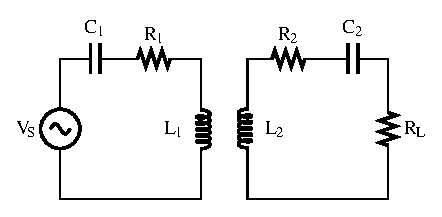
\includegraphics{./images/SS}\label{F:SS}} 
\subfigure[SP]
{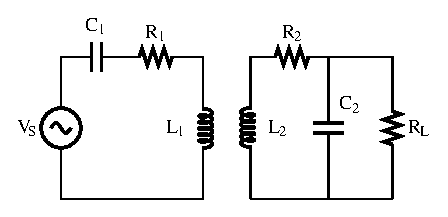
\includegraphics{./images/SP}\label{F:SP}}
\subfigure[PS] 
{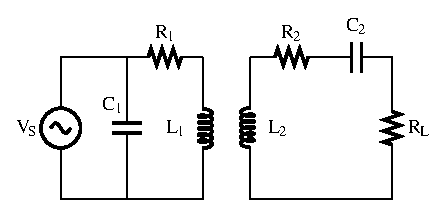
\includegraphics{./images/PS}\label{F:PS}} 
\subfigure[PP]
{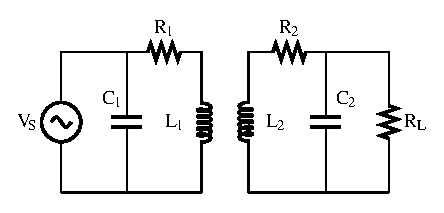
\includegraphics{./images/PP}\label{F:PP}}
\end{subfigmatrix}
\caption{Compensation topologies}
\label{F:topologies}
\end{center}
\end{figure}

In this section each topology is evaluated in a detailed way to determine their advantages and drawbacks, and then, to conclude which is the most suitable topology according to our application. Therefore, the equations determined in Section \ref{subsec:Model} will be changed due to the insertion of the compensation capacitors, depending on the used topology. This new equations are listed in Appendix \ref{Appendix: A}. 

Eventually the best topology in terms of maximum transferred power will be chosen. Arbitrary values are selected from the system parameters represented in Table \ref{T:ArbitraryValues}. 

\begin{table}[h]
\begin{center}
\begin{tabular}{|c|c|}

\noalign{\global\arrayrulewidth1pt}
\hline
\textbf{Parameter} & \textbf{Value}\\
\hline
\hline
$V_S$ 	& 5 V\\ \hline 
$R_S$   & 50 $\Omega$\\ \hline
$R_1$   & 0.5 $\Omega$\\ \hline
$R_2$ 	& 0.5 $\Omega$\\ \hline
$R_L$ 	& 50 $\Omega$\\ \hline
$L_1$ 	& 10 $\mu$H \\ \hline
$L_2$ 	& 10 $\mu$H \\ \hline
$C_1$ 	& 2 nF \\ \hline
$C_2$ 	& 2 nF \\ \hline
$M$ 	& 3 $\mu$H \\ \hline     
\end{tabular}
\caption{Arbitrary values of the electric parameters}
\label{T:ArbitraryValues}
\end{center}
\end{table}


All the calculations for computing the efficiency and the output power (load power) are done using the alternating current basics. Thus, the input power $P_{in}$ and the load power $P_{L}$ are given by,

\begin{equation}
P_{in} = V_{in}\cdot{I_{in}}\cdot{cos(\varphi)}
\end{equation}

\begin{equation}
P_{L} = ( I_{L} ) ^2\cdot{R_L}
\end{equation}

where $\varphi$ is the phase between the input voltage and the primary current. In the previous equations, it is used the root mean square (\textit{RMS}) for $V_{in}$, $I_{in}$ and $I_L$; as a consequence, the power results are expressed in its average value.  Note that $P_{in}$ is multiplied by the power factor $cos(\varphi)$ which corresponds to compute the active power or consumable power.

\subsubsection{SS topology}

The equivalent circuit of the SS topology can be determined by gathering the expression of $Z_R$ with $Z_{eq}$ listed in Appendix \ref{sec:secondaryS} and \ref{sec:primaryS} respectively. By varying the frequency, the efficiency $\eta$ and the output power (load power) will show their maximum at the resonance frequency. 

In Figure \ref{F:effTopologies}, when the frequency grows, the efficiency tends to a constant value that depends on the system parameters. This statement does not mean that is optimal to work at high frequencies because the output power drops sharply when the frequency overtakes the resonance frequency. The explanation is that the input power also falls with the same magnitude as the output power.

Another interesting parameter for studying in each topology is the equivalent impedance of the system. This impedance will help us to determine the optimal compensation for our application because its behavior depends on the operating frequency. Figure \ref{F:SSimpedance} shows that at the resonance frequency, the whole imaginary part of $Z_{eq}$ is canceled and the system impedance is purely resistive. The impedance of this compensation topology behaves as a capacitance since the the frequency increases to the resonance frequency; from this point, it will behave as an inductance.


\begin{figure}[h!]
\begin{center}
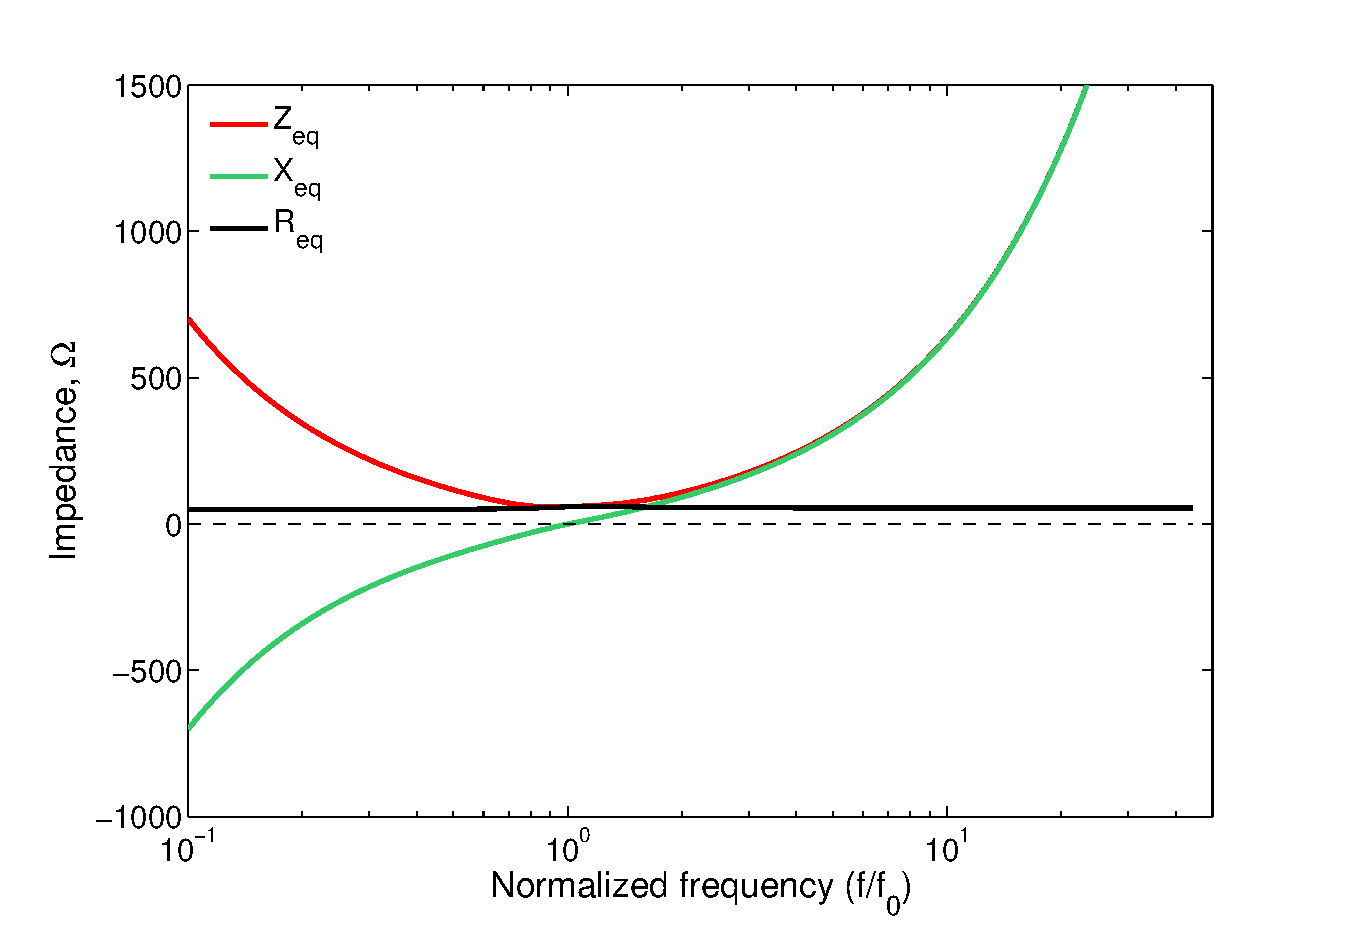
\includegraphics[width=0.7\textwidth]{./images/SS_impedance} 
\caption{Equivalent circuit impedance w.r.t frequency for SS topology}
\label{F:SSimpedance}
\end{center}
\end{figure}

% \\
\subsubsection{SP topology}

It is possible to model the SP topology using the formulas obtained for $Z_R$ and $Z_{eq}$ in Appendix \ref{sec:secondaryP} and \ref{sec:primaryS} respectively. As it is explained in Appendix \ref{sec:secondaryP}, to transfer the maximum power to the system load, is recommended to delete the imaginary part of $Z_R$. This is done by changing the secondary capacitor value to a value that can be computed using the Equation \ref{Eq:differentCapacitor}, allowing to transfer only consumable power to the load. As a consequence, the maximum efficiency and load power will be at a different frequency than the resonance frequency of the whole system\footnote{The system resonance frequency in this case will be a trade-off between the resonance frequency of both primary and secondary circuits due to the different capacitance used.}. The impedance's model has a similar curve as in case of the SS topology impedance as Figure \ref{F:SPimpedance} shows.

\begin{figure}[h!]
\begin{center}
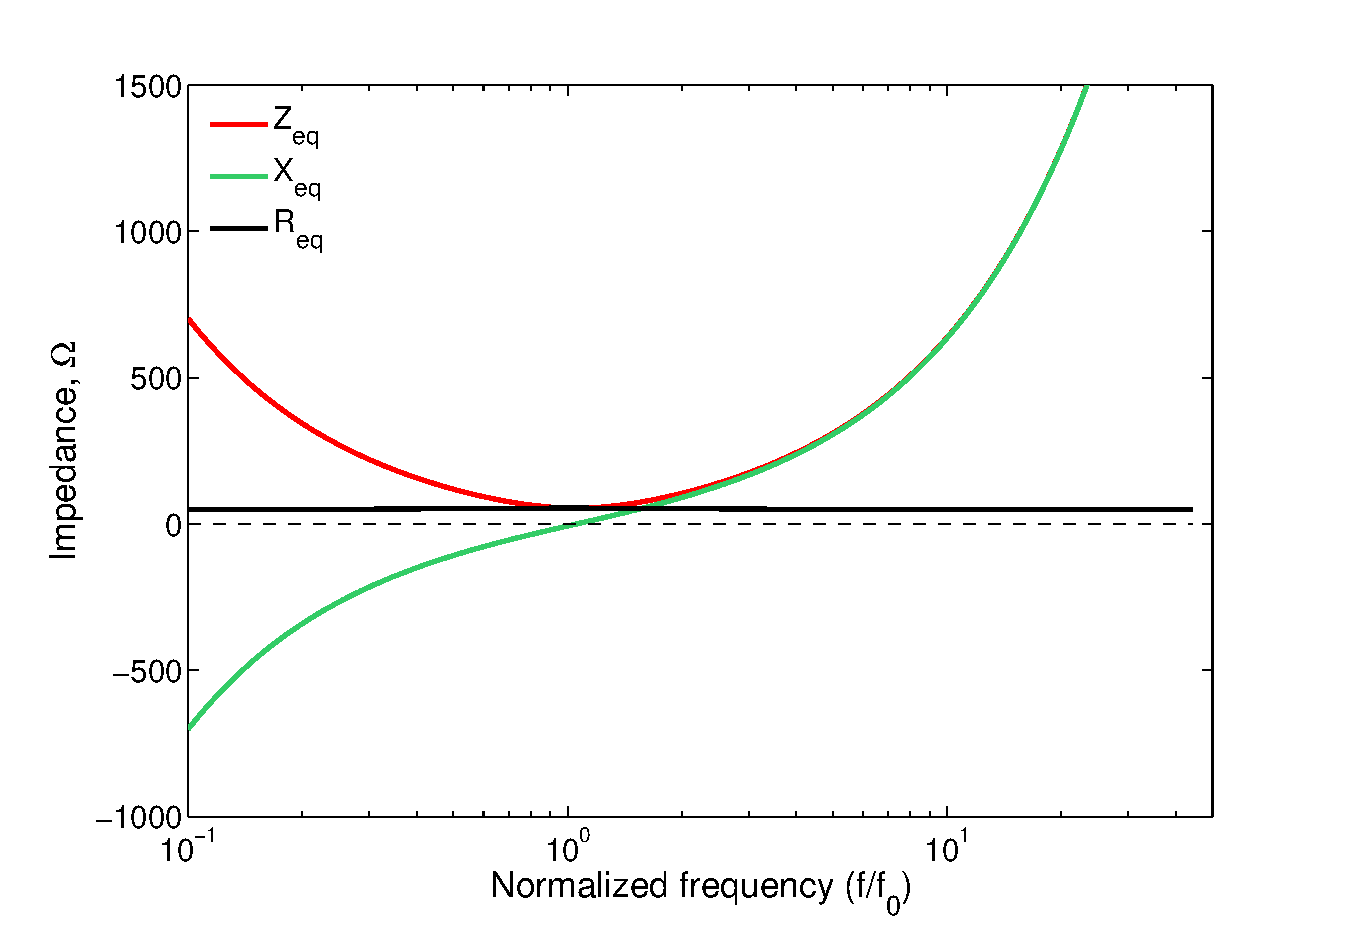
\includegraphics[width=0.7\textwidth]{./images/SP_impedance} 
\caption{Equivalent circuit impedance w.r.t frequency for SP topology}
\label{F:SPimpedance}
\end{center}
\end{figure}

\subsubsection{PS topology}

The SP topology are modeled with the equations for $Z_R$ and $Z_{eq}$ listed in Appendix \ref{sec:secondaryS} and \ref{sec:primaryP} respectively. A parallel capacitor is generally used to generate large currents in the primary coil \cite{meyer}. An interesting point for the parallel primary topologies is that the voltage delivered from the source is the same voltage applied to the capacitor.

Note that as in case of the secondary capacitor in parallel, the equivalent impedance of this topology shows a reactance, as it is explained in Appendix \ref{sec:primaryP}. This imaginary part has to be deleted whether is wanted to transfer the maximum power. In this case, the optimal capacitor will be the obtained in Equation \ref{Eq:differentCapacitor2}. Hence, the system will resonate at a different frequency than the resonance one. This new capacitor has an important dependence on the selected secondary topology because it is inversely proportional to the $Z_R$.

In this topology, the total impedance shifts from an inductive circuit at low frequencies to a capacitive circuit at high frequencies. At the resonance frequency, the equivalent impedance becomes purely resistive and reaches its maximum vale. This is an important fact to be taken into account when  is going to be used a parallel primary topology, because the power transfer can be maximized only by having a current source input \cite{delft}. Nevertheless, in this project is only used a sinusoidal voltage source to drive the system.

\begin{figure}[h!]
\begin{center}
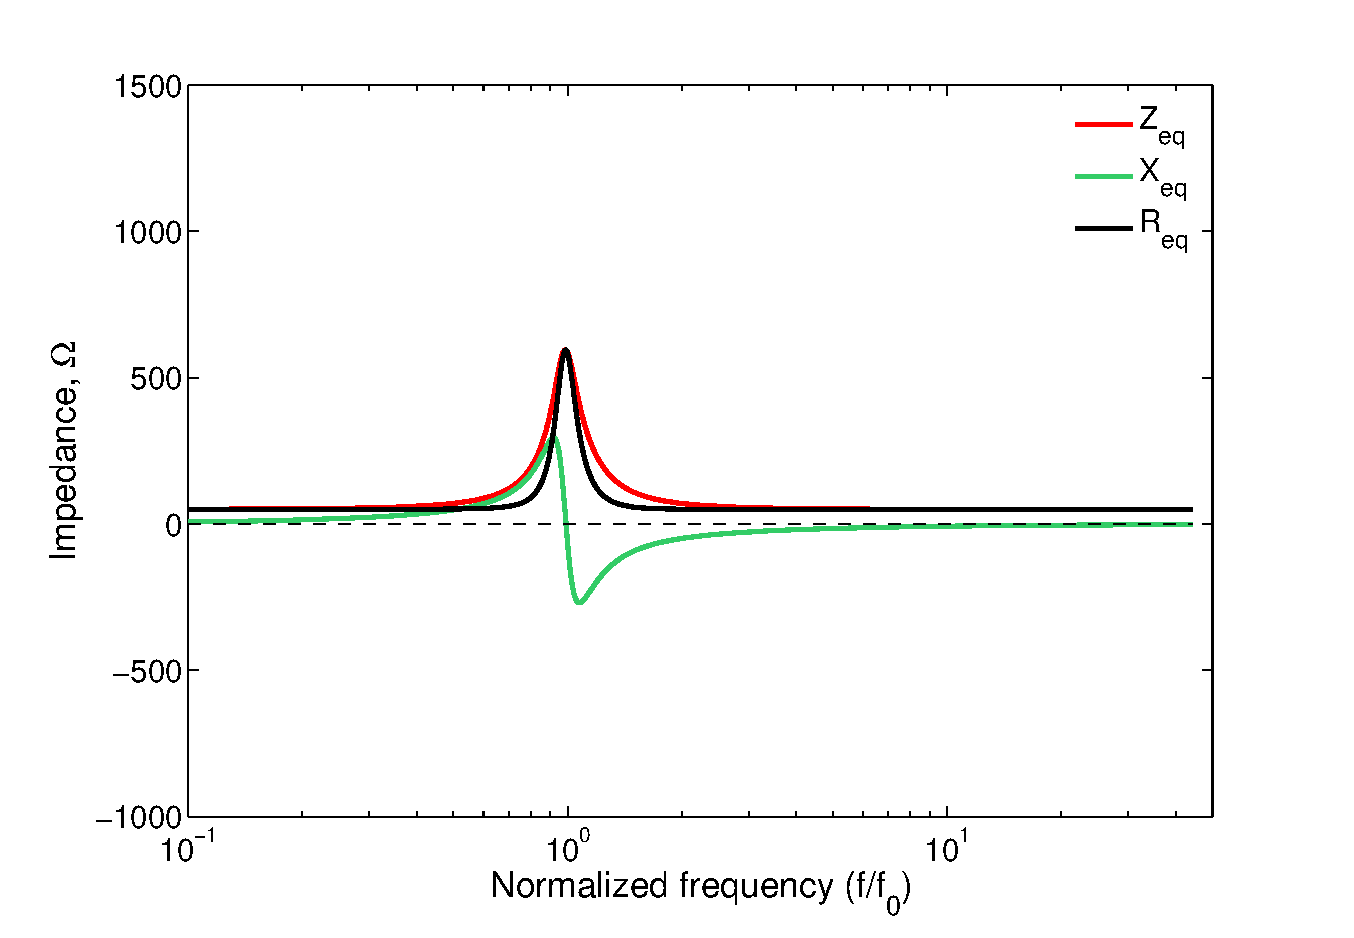
\includegraphics[width=0.7\textwidth]{./images/PS_impedance} 
\caption{Equivalent circuit impedance w.r.t frequency for PS topology}
\end{center}
\end{figure}

\subsubsection{PP topology}

Finally, the PP topology can be obtained through the equations for $Z_R$ and $Z_{eq}$ listed in Appendix \ref{sec:secondaryP} and \ref{sec:primaryP} respectively. This topology is well suited to supply a stable secondary load current due to parallel position of the secondary capacitor \cite{meyer}.
In Figure \ref{F:PoutTopologies} this point is verified when the frequency increases from the resonant one.

\begin{figure}[h!]
\begin{center}
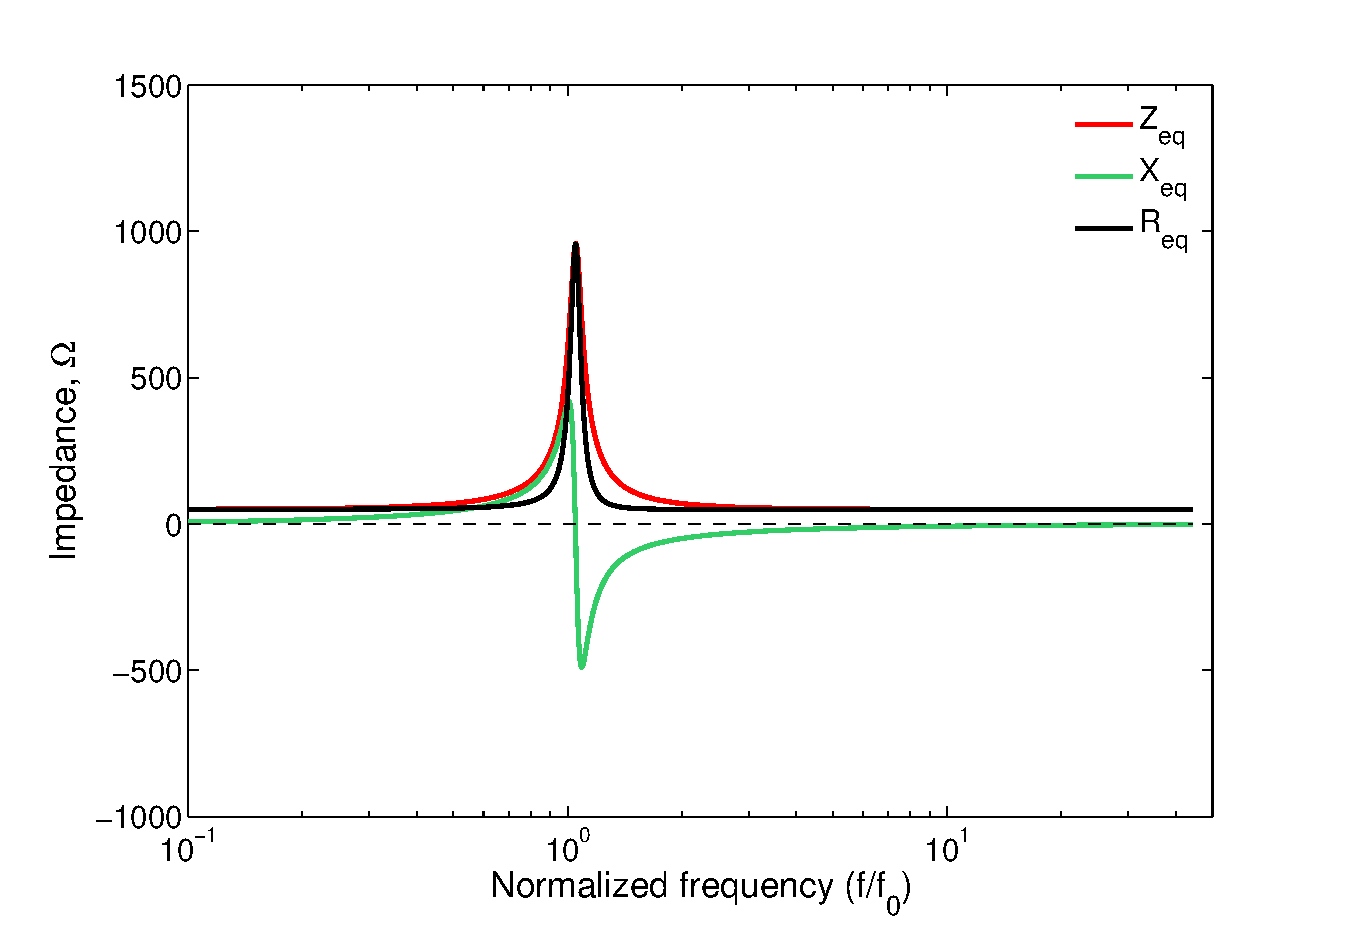
\includegraphics[width=0.7\textwidth]{./images/PP_impedance} 
\caption{Equivalent circuit impedance w.r.t frequency for PP topology}
\end{center}
\end{figure}


The WPT system for this topology will be subjected in the same conditions as in case of the PS topology. Hence, is optimal to drive it with a current source due to its great impedance at the resonance frequency.

\subsubsection{Discussion}\label{subsec:discussion2}

In this section the comparison between each topology is done. The choice of the optimal compensation topology will be made depending on the power levels for a given system load. With the system parameters values, tabulated in Table \ref{T:ArbitraryValues}, the expressions of the efficiency and output power are expressed in Figures \ref{F:effTopologies} and \ref{F:PoutTopologies}. 


\begin{figure}[h!]
\begin{center}
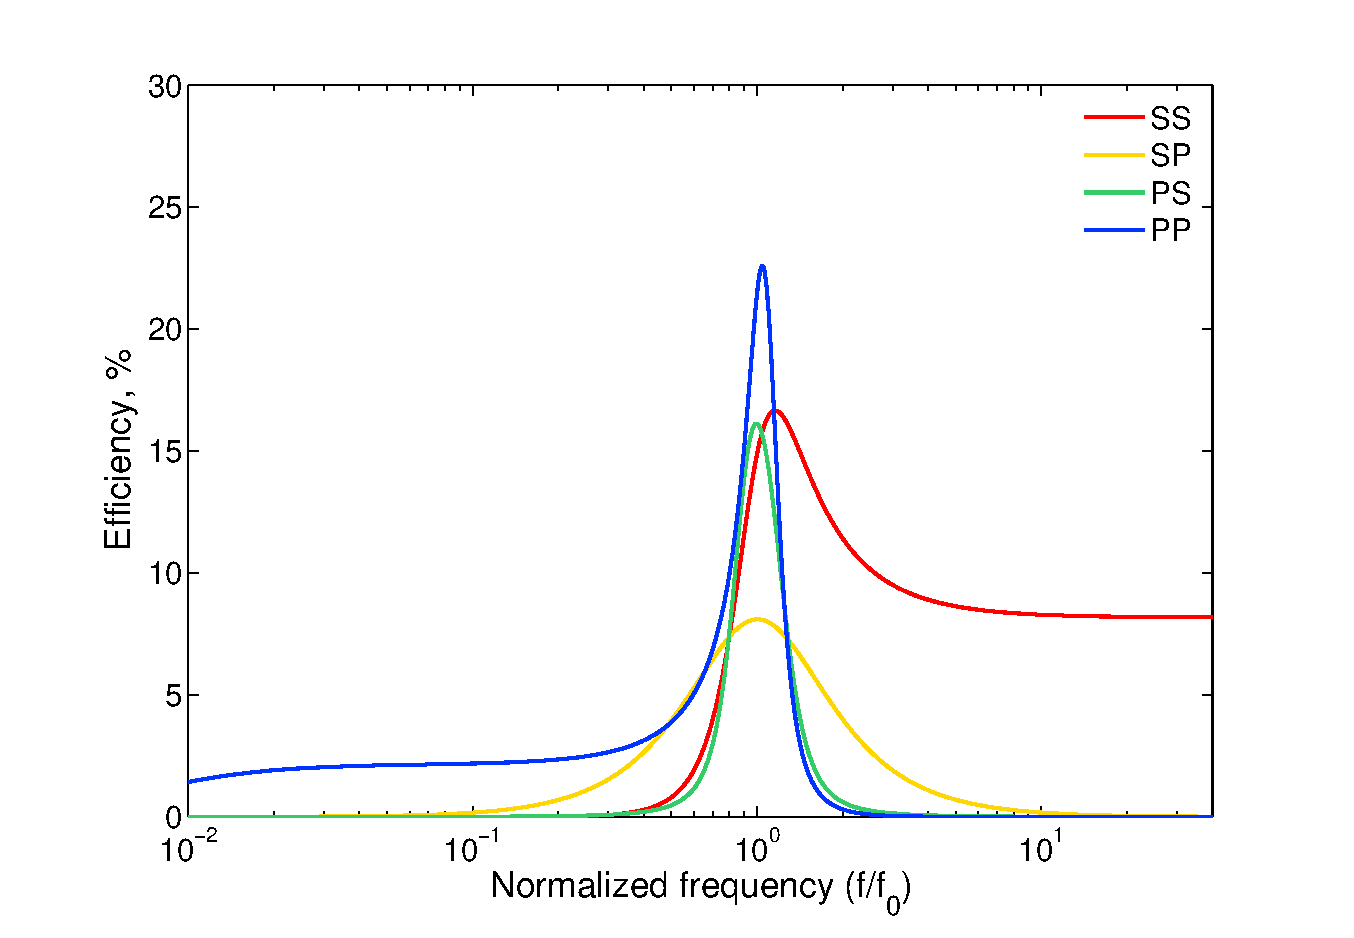
\includegraphics[width=0.7\textwidth]{./images/effModel} 
\caption{Efficiency for all topologies}
\label{F:effTopologies}
\end{center}
\end{figure}

\begin{figure}[h!]
\begin{center}
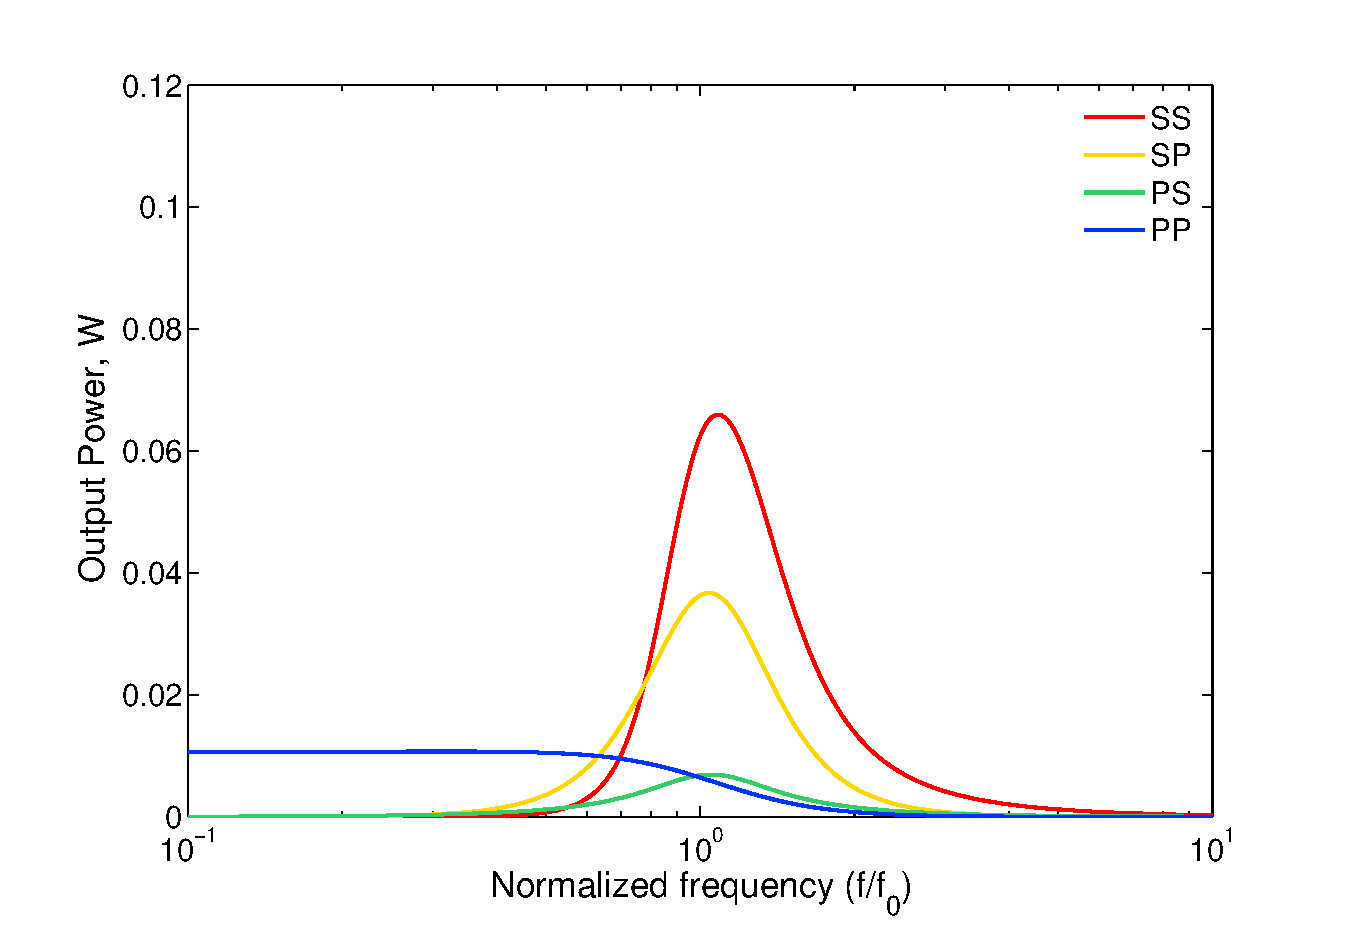
\includegraphics[width=0.7\textwidth]{./images/PoutModel} 
\caption{Output power for all topologies}
\label{F:PoutTopologies}
\end{center}
\end{figure}

The previous figures show that, for the chosen parameters, the optimal topology in terms of output power is the SS topology. The primary series topology has the characteristic that the compensator capacitor does not depend on the load, so it is a good option to select when the loading profile is variable. By comparing the two primary series topologies, when the load becomes higher it is optimal to select a SP topology because the more load resistance, the higher output power levels. This statement can be verified looking at Figure \ref{F:SloadDependance}. 

\begin{figure}[htb]
\begin{center}
\begin{subfigmatrix}{2} 
\subfigure[$R_L = 100\Omega$]
{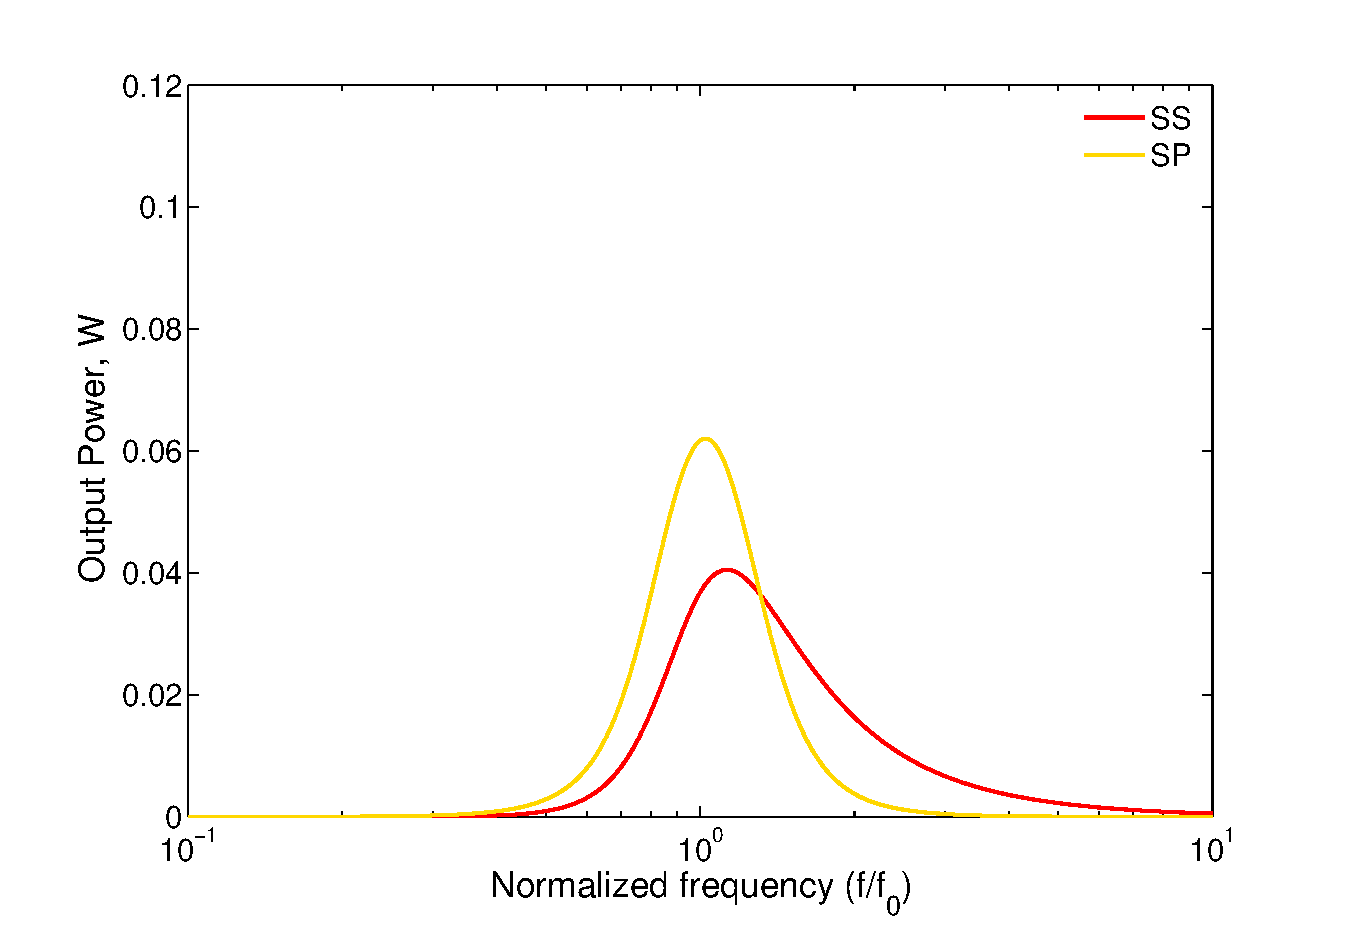
\includegraphics{./images/SS_SP_pout_100}\label{F:S100}} 
\subfigure[$R_L = 1000\Omega$]
{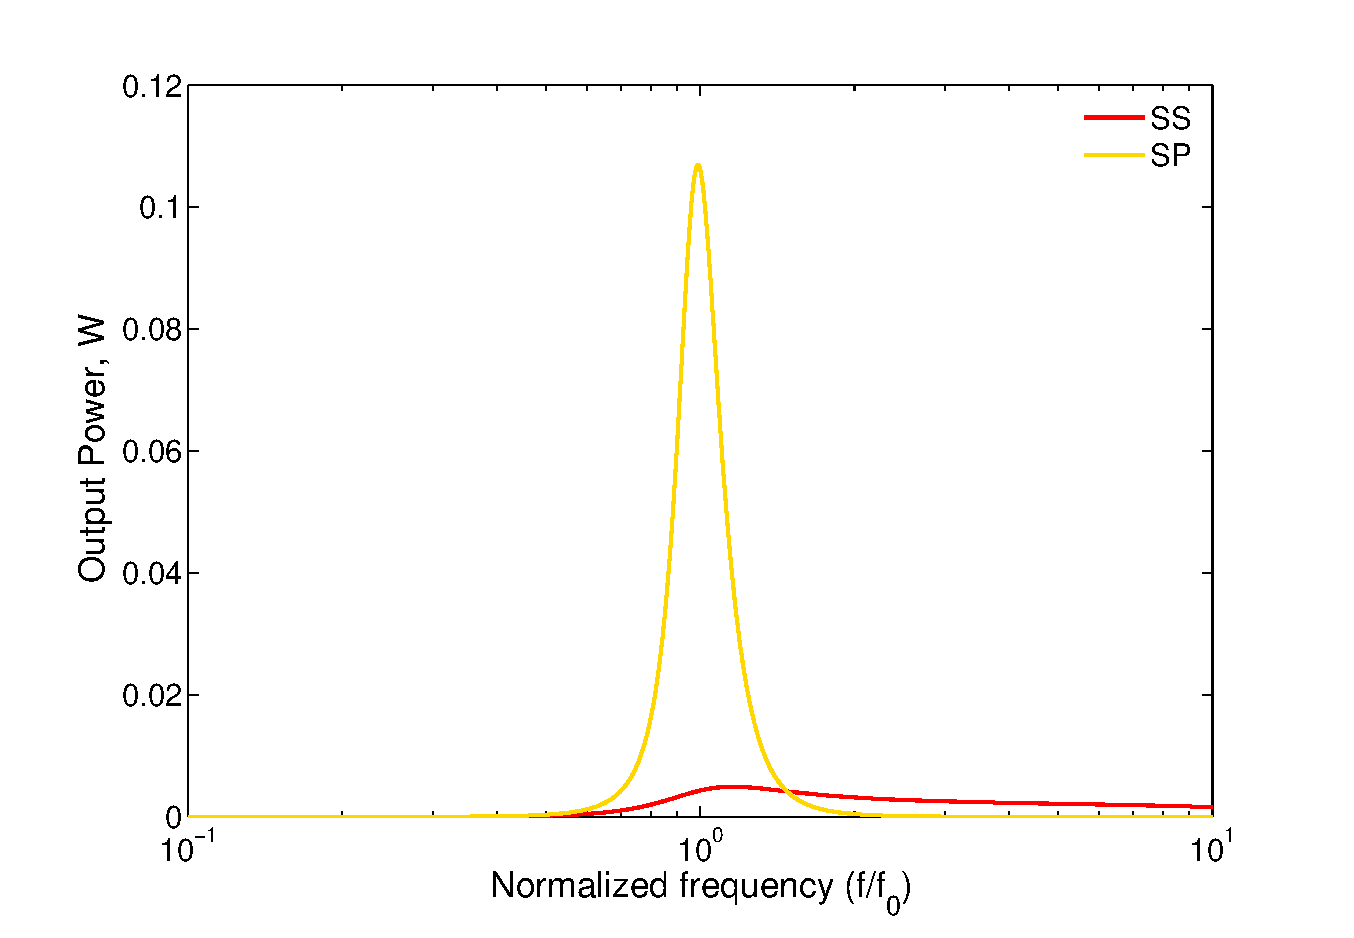
\includegraphics{./images/SS_SP_pout_1000}\label{F:S1000}}
\end{subfigmatrix}
\caption{Output power for SS and SP topologies varying the load resistance}
\label{F:SloadDependance}
\end{center}
\end{figure}

For primary compensated topologies, the compensator capacitor varies with the system load whether is desirable to transfer maximum consumable power at a specific frequency. The output power for these topologies increases when the system load becomes small. In Figure \ref{F:PloadDependence}, the power roughly increases for a PS topology for a small system load but with a lower frequency tolerance. In contrast, a PP topology has a high frequency tolerance in terms of output power. If the system has not a good frequency stability, the best topology to select is the PP topology.

\begin{figure}[htb]
\begin{center}
\begin{subfigmatrix}{2} 
\subfigure[$R_L = 100\Omega$]
{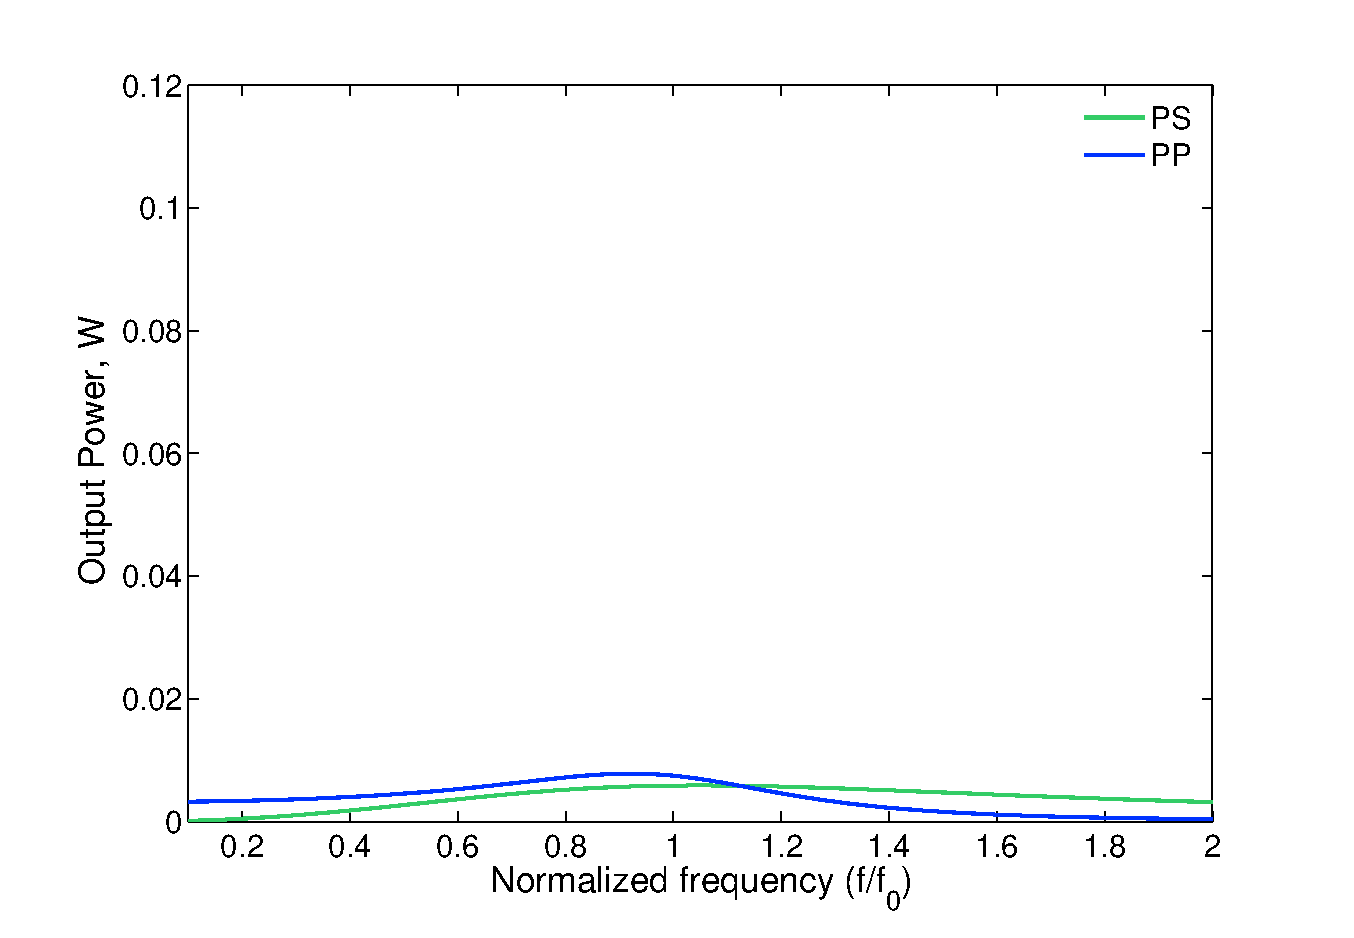
\includegraphics{./images/PS_PP_pout_100}\label{F:P100}} 
\subfigure[$R_L = 1000\Omega$]
{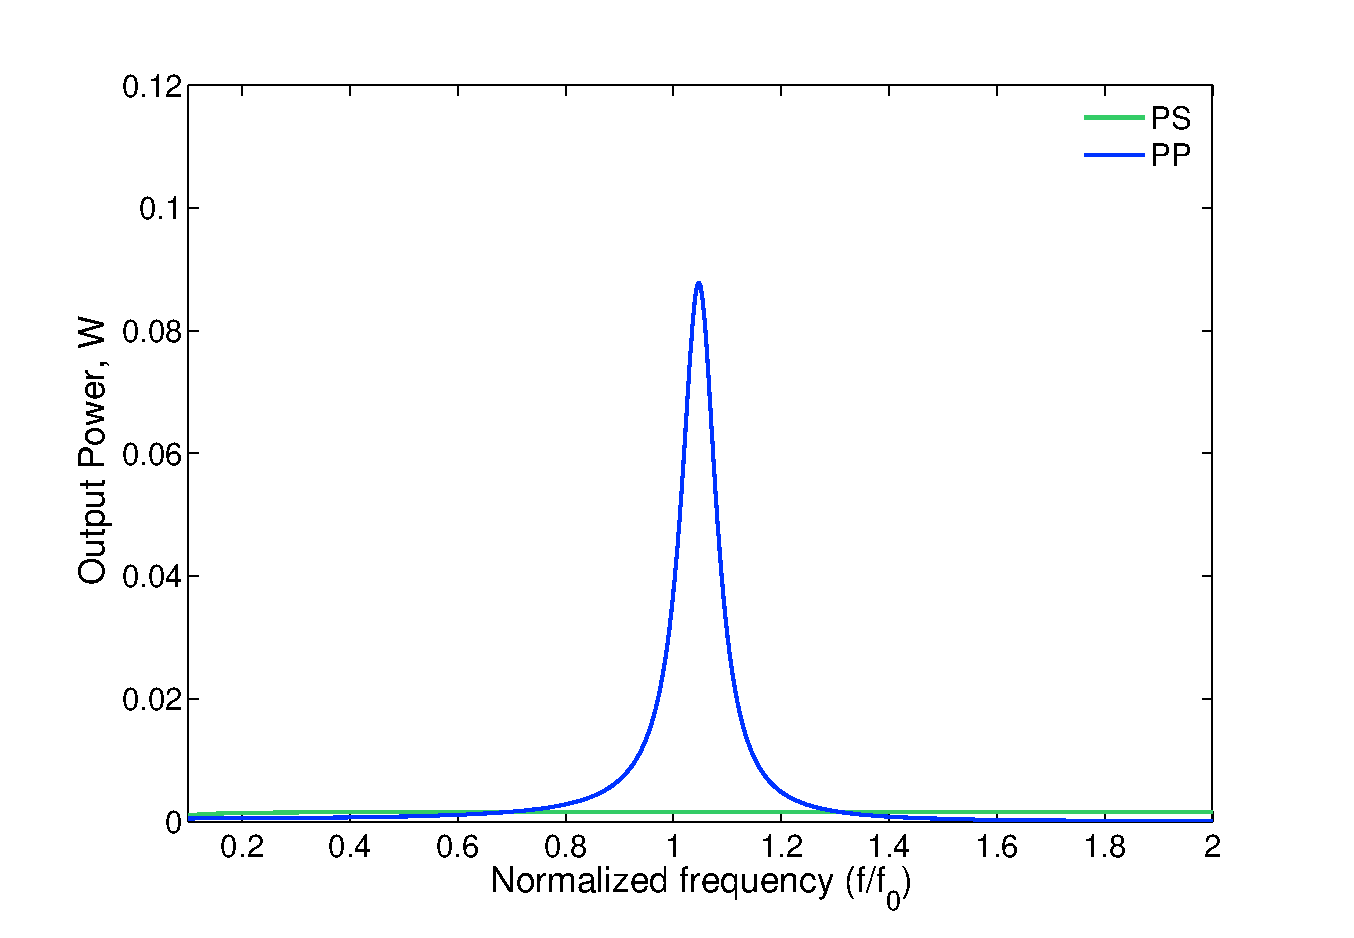
\includegraphics{./images/PS_PP_pout_1000}\label{F:P1000}}
\end{subfigmatrix}
\caption{Output power for SS and SP topologies varying the load resistance}
\label{F:PloadDependence}
\end{center}
\end{figure}

As previous figures show, the worts topology in terms of output frequency is the PS topology. Then, this topology is rejected for using in the studied application. The remaining topologies have good power levels but only one can be selected.

For low load resistances, the better option is the SS topology and is the best manner to transfer energy because both primary and secondary capacitors delete the imaginary parts of impedance allowing to transfer active power. 

When the load resistance increases, secondary parallel capacitors are necessary. To select between SP or PP topologies, we are focused in the effect of the primary capacitors. PP topology generates more amount of reactive power (losses) than SP topology with resonant capacitor, due to the parallel capacitor position on both sides. As a result, the second selected topology is SP topology.

In following sections is discussed the performance of these two topologies and is determined which is the most suitable form to place the compensation capacitors.















	\section{Design Considerations}
Wireless power transfer is a promising way of transfer energy which is said to extend and create new applications restricted in past because of energy issues. By implementing the coupling system on a nano-quadcopter we are trying to enlarge this list of applications. Nevertheless, this attempt of bringing WPT to a new dimension using a nano-quadcopter have involved serious payload constraints.

		\subsection{Power Level}
The power level describes how much power the system is dealing with. We focus on the input and output power of the system, $P_{in}$ and $P_{out}$ respectively, which define induction efficiency. 

\begin{equation}
	\eta = \frac{P_{out}}{P_{in}}
\end{equation}

Although a high power level is not a priority, it is necessary to have at least the boundary power value necessary for running the final application. Whether this power level is higher as the desired it will mean that the distance $z$ (which is referred to the axial distance) could be increased. 

While power level is smaller than expected, it would be necessary to increase at least one of the following parameters in order to rise the transferred power:
\begin{itemize}[noitemsep] % To be more compact --> \begin{itemize}[noitemsep,nolistsep]
	\item Mutual inductance
	\item Voltage induced in the secondary coil
	\item Current through the primary coil 
\end{itemize}

The three parameters are quite related among them. The first one, mutual inductance is strongly dependent on the distance ($M\propto{1/z^3}$). Thus, the first and easiest solution is reduce the axial distance between coils. The second possibility is to increase the induced voltage in the secondary coil, which is proportionally to the operating frequency. Eventually, the magnetizing current through the primary coil can rised by decreasing the operating frequency. This may sound weird since the power transferred can be increased by either decreasing or increasing frequency. A trade-off should be sought to maintain the output power without compromising the transfer distance.

%%
Another important point to consider, once distance and frequency are established, is impedance matching. As we said in Section \ref{subsec:Model} the maximum transfer power occurs when there is an impedance matching between $Z_1$ and $Z_R$. Taking into account that the only variable parameter inside the $Z_R$ expression is the resistance of the load $R_L$, it will be necessary to define the most suitable load value. Note that the reflected impedance depends on $R_L$ and distance, which is expressed by mutual inductance $M$. This lead to define an average value of $R_L$ for an specific range of distances.
%%


% 		\subsubsection{Safety Issues}
% This is closely related to power level. In comparison to wired power systems, WPT systems suffers from unique safety issues. One of the concerns is the risk caused by the expose to electromagnetic radiation. The exposure to low-frequency electric and magnetic fields results in negligible energy absortion and no measurable temperature rise in the body.




		\subsection{Quality Factor}
The quality factor or Q factor is a dimensionless parameter that describes how under-damped a power antenna is; the higher Q factor, the less damping there is. Thus, both \textit{Tx} and \textit{Rx} coils are intended to have great Q factor values because the higher the Q factor are, the higher the transfer efficiency will be \cite{medical}. Q factor at the same time is the response to the previous power trade-off between a higher frequency and therefore higher induced voltage or lower frequency and a greater magnetizing current, and it defined as:

\begin{equation}
	Q = \frac{\omega{L}}{R}=\frac{\omega_0}{\Delta{\omega}}
	\label{eq:Qfactor}
\end{equation}

$Q$ depends on the applied frequency $2\pi{f}=\omega$, the inductance value $L$ and the resistance of the coil $R$. Occasionally radiation resistance $R_{rad}$ is included in the denominator \cite{5413106}. As stated before in Section \ref{subsec:coilResistance} this resistance can be neglected. Q factor also can be seen as a selectivity factor, that is why it is sometimes defined as the quotient of natural frequency $\omega_0$ by the bandwidth $\Delta{\omega}$. 

Q factor is an image of the quality of a given coil. It defines its capacity to generate a large magnetic field and low losses \cite{meyer}. According to \cite{Consortium}, a quality factor below 10 represents a really poor coil that should be avoided for WPT, and values around 100 are excellent for industrial applications. \textit{Good} coils will permit higher operating frequencies, while coils with small Q factor will tend to transfer at lower frequencies as is shown in the next figure.

\begin{figure}[h]
\begin{center}
	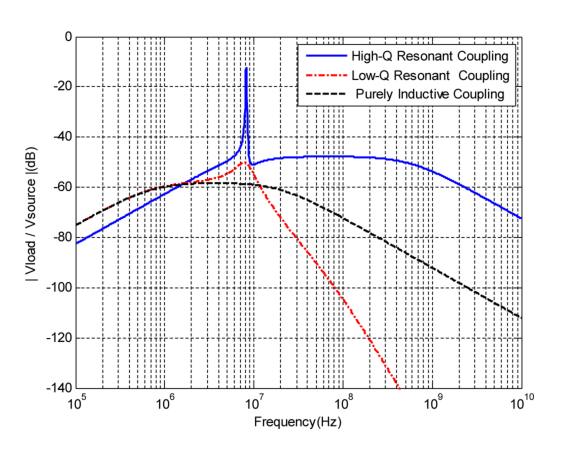
\includegraphics[width=0.7\textwidth]{./images/mit2}
\caption{Voltage transfer function over frequency for different systems}
\label{F:Qfactor}
\end{center}
\end{figure}

From Figure \ref{F:Qfactor} it can be observed three different inductive coupling systems. The high-Q resonant coupling has the highest Q factor, and therefore the narrower bandwidth. Note that in some applications, such as ours, the Q factor is not always the higher, the better. A really high Q factor above 1000, achieved by using open-ended helical coils like in \cite{Karalis200834}, involves a tight bandwidth. Since the resonant frequencies of Tx and Rx coils can not be identically the same, a too narrower band could cause mistuning. In the above figure it can be noticed the huge difference between a pure inductive system and a resonant one. It must be remarked for resonant systems that after their resonant frequency, the overall performance is cut down.


















		\subsection{Coupling Factor}
Together with Q factor, the coupling factor is the most typical parameter to describe air-core transformers. It is expressed as follows:

\begin{equation}
	k = \frac{M}{\sqrt{L_1L_2}}
\end{equation}

This performance parameter measures the fraction of magnetic flux generated by the \textit{Tx} coil is penetrating the \textit{Rx} coil. The more flux reaches the \textit{Rx} coil, the better the two coils are coupled. This level of coupling is expressed by the coupling factor $k$. It varies between 0 and 1. For $k=0$ the two coils are completely decoupled, while the ideal $k=1$ would mean totally coupled coils.

Coupling factor is determined by the size and the position of primary and secondary coils. In Section \ref{subsec:geo} it is discussed the better coils dimension with the purpose to maximize the coupling between them.













		\subsection{Operating Frequency} \label{subsec:operatingFreq}
The operating frequency is another important design consideration in the WPT system. This frequency describes the rate of generation of the electromagnetic waves by the primary coil. For sure, the secondary coil must be designed to work at the operating frequency. As mentioned earlier in Section \ref{subsec:seriesResonance}, to work at resonance it is necessary to drive the primary coil from an external source, in our case it will be an oscillator the responsible of producing the periodic sine wave, \textit{oscillating} at the same operating frequency.

Determine the ideal operating frequency is not possible without knowing many factors as, coil sizes, Q factors, self-resonant frequency, efficiency, etc. Hence, it is intended to determine the suitable frequency band in which the coils could work properly. This frequency range takes into account either the upper and lower frequency boundaries. 

The upper limit is restricted by the maximum switching frequency of the transmitter power driver (red dashed line in Figure \ref{F:frequency}). Another limitation at high frequencies is the one related to coil self-resonance frequency ($f_s$), and so the parasitic capacitance of the coils. Initially any coil is designed to work at $f_s$ to provide the highest possible Q factor. 

Exciting the windings with an excitation frequency of approximately 10$\%$ of $f_s$ will ensure that the parasitic capacitive effects will not influence the inductor impedance values, and that the parasitic capacitances can be removed from the inductor model shown in Figure \ref{F:modelingCoil} \cite{tesis}. Owing to the fact that the experimental results of $f_s$ are not higher than 30 MHz, the maximal operating frequency is set to be at least 5 times lower than the self resonance frequency, as follows,

\begin{equation}\label{eq:maxop}
f\leq\frac{f_s}{5}
% f\simeq\frac{f_s}{5}
\end{equation}

For low frequencies there are no restrictions, but recommendations. The \textit{Wireless Power Consortium} suggests as admissible, Q factor values above 100 for WPT applications. To achieve the desired Q factor, frequencies higher than 500 kHz are typically needed.

\begin{figure}[h]
\begin{center}
	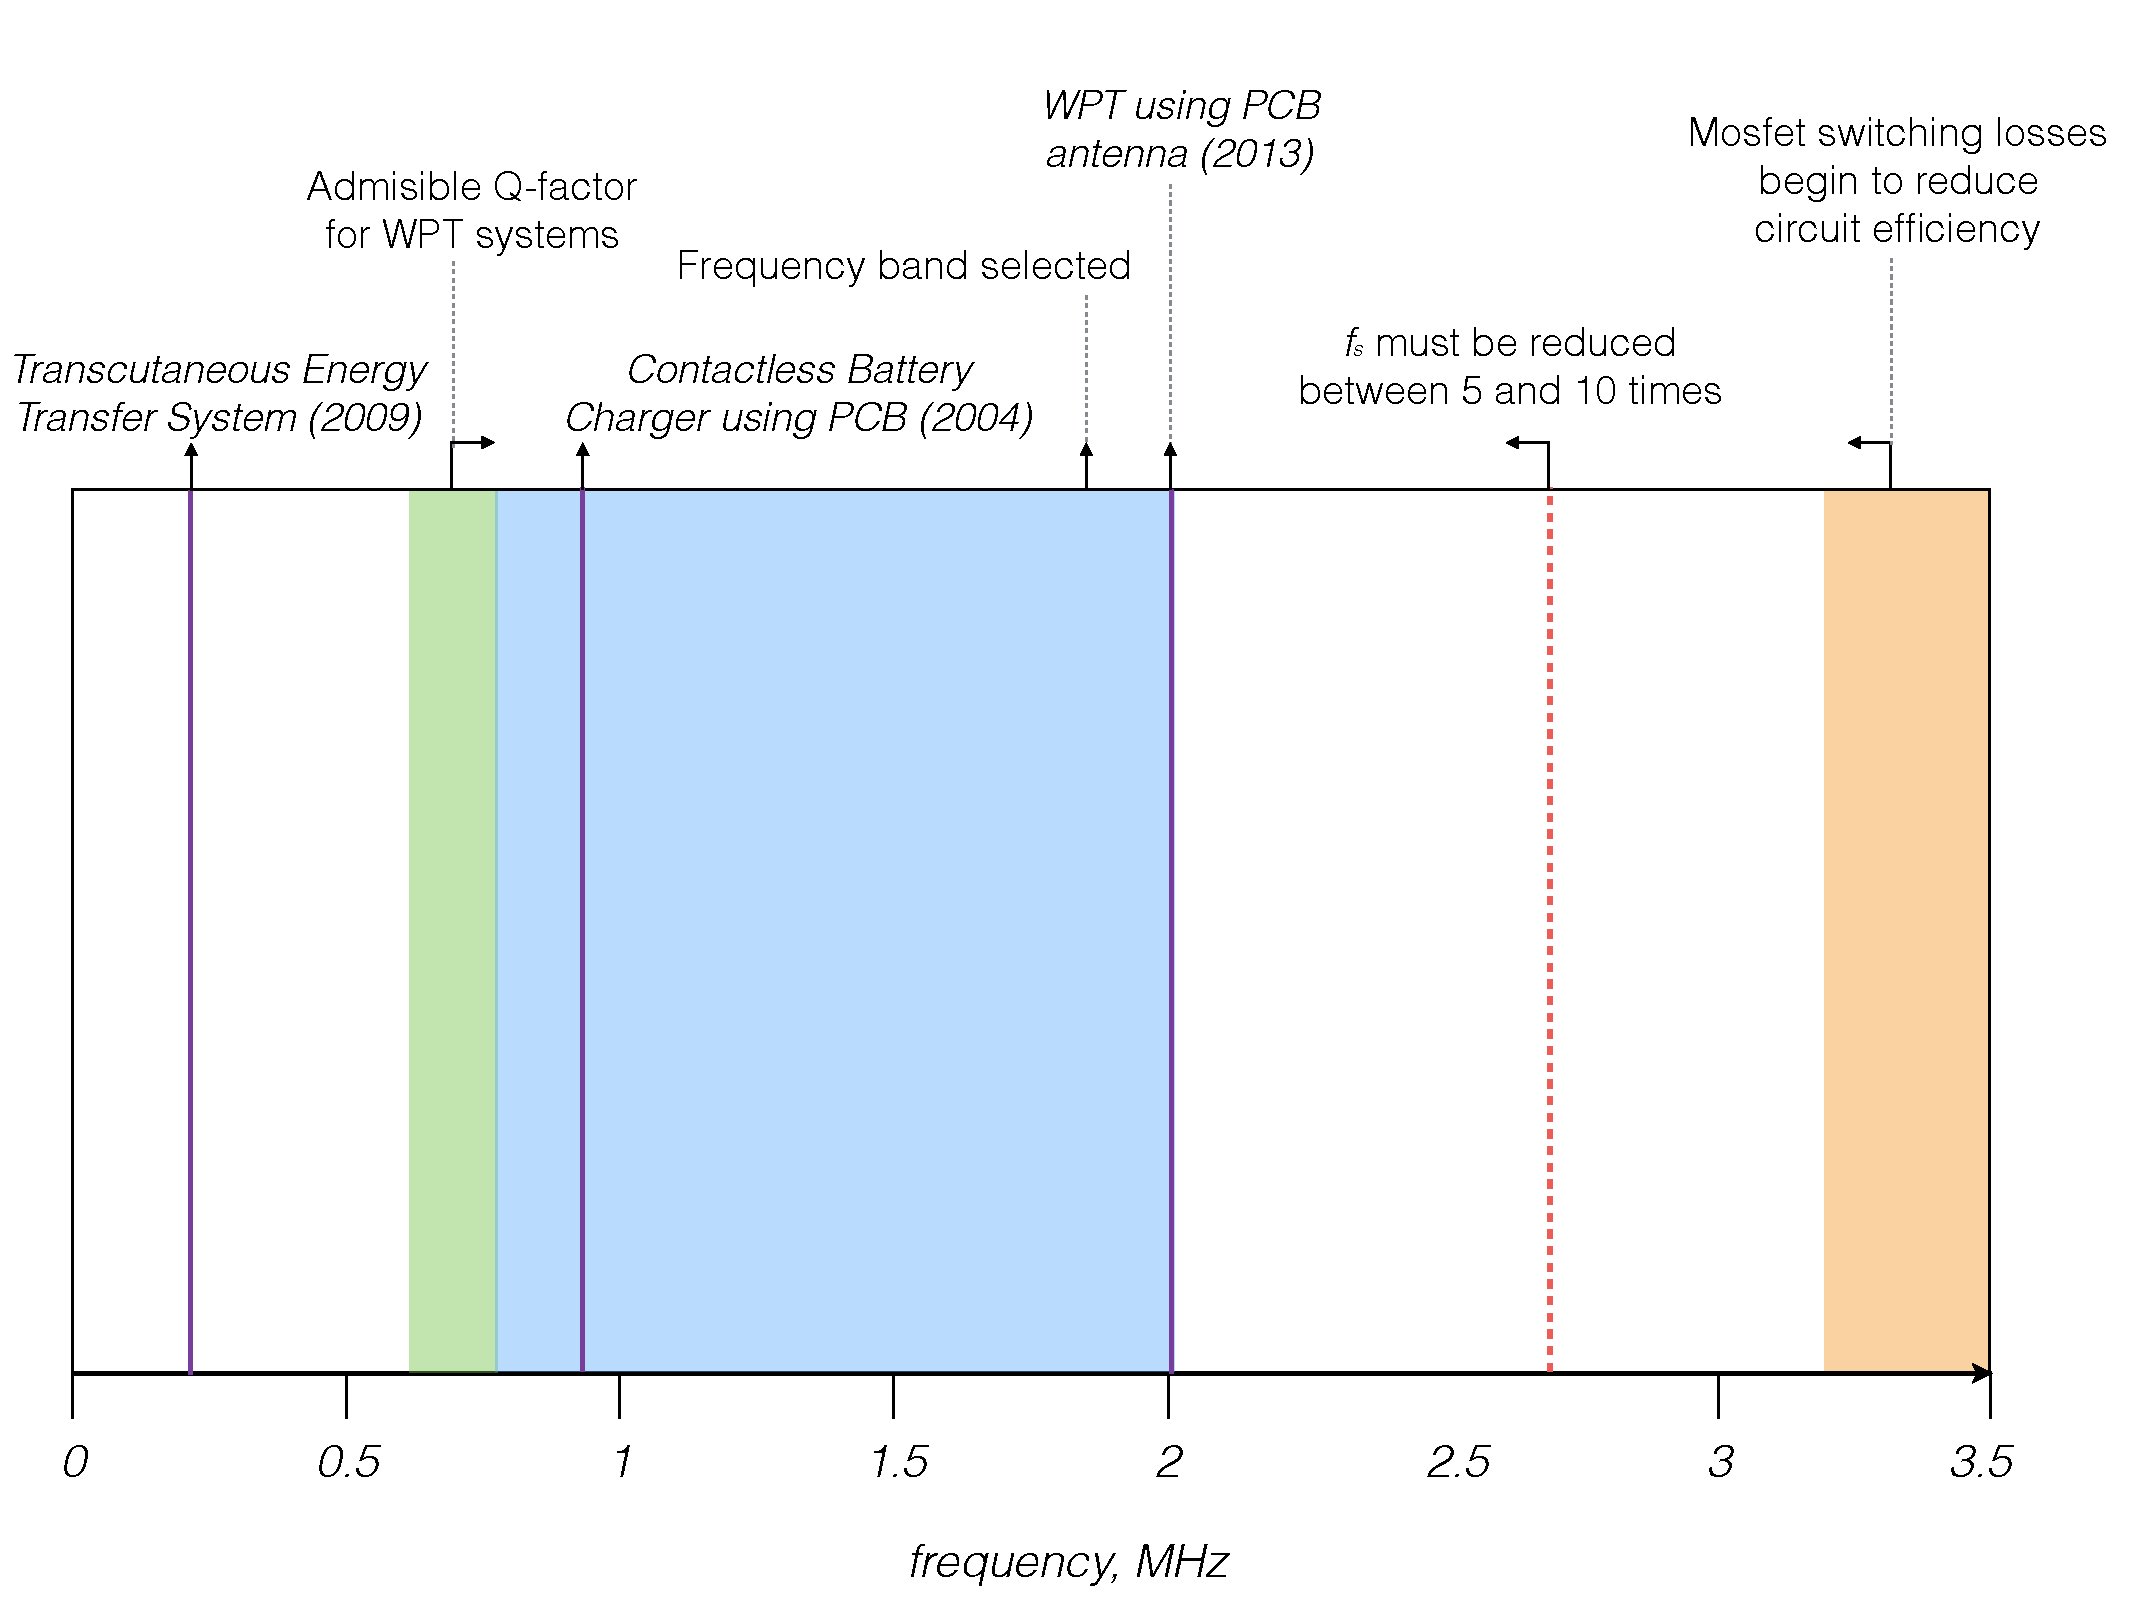
\includegraphics[width=0.95\textwidth]{./images/frequency}
% \vspace{-1.5em}
\caption{Frequency band constraints}

\label{F:frequency}
\end{center}
\end{figure}

Figure \ref{F:frequency} shows the specific frequency band for coils' diameters between 3 and 10 cm which is the desired order of magnitude of the coils. The vertical purple lines indicate different\footnote{Transcutaneous Energy Transfer System \cite{keynote1}, Contactless Battery Charger using PCB \cite{keynote2} and WPT using PCB antenna \cite{keynote3} are useful examples to consider when selecting the operating frequency.} works based on WPT systems similar as ours in terms of transfer distance and coil sizes.

Having set the frequency boundaries and some WPT example applications, for this work the frequency band between 700 kHz and 2 MHz is studied for the next proposed systems.












\subsection{Size and Weight} 
In order to study the behaviour of coils depending on the different coil parameters, such as coil diameter, number of turns, metal conductor or conductor diameter, different models have been designed and tested.

Before knowing power specifications, coil outfitting supports or drone's stability limitations we began to design the power coils. Using a nano-quadcopter as carrying system and resonant induction as mean of power transfer, we set a goal in transferring power up to 20 cm. We chose these range of distances based on previous works \cite{TypicalL}\cite{UAV}\cite{flowchart}\footnote{All the publications selected are similar with regards to operating frequency.}. In front of a design with at least four freedom degrees we decided to fence each variable to reduce the number of possible coil designs.

\begin{table}[ht]
\begin{center}
\begin{tabular}{|c|c|}

\noalign{\global\arrayrulewidth1pt}
\hline
\textbf{Parameter} 	& 	\textbf{Definition}\\
\hline
\hline
$R$ 		& Coil radius		\\ \hline 
$D$  		& Coil diameter		\\ \hline
$A$ 		& Coil area 		\\ \hline 
$d$  		& Wire diameter		\\ \hline 
$l$  		& Wire length		\\ \hline
$S$ 		& Wire section		\\ \hline 
$h$ 		& Coil height		\\ \hline
$z$			& Axial distance	\\ \hline
$N$			& Number of turns 	\\ \hline
$m$			& Coil mass 		\\ \hline  
\end{tabular}
\caption{Geometric parameters of coil models.}
\label{T:coil parameters}
\end{center}
\end{table}

				\subsubsection{Coil Shape}
Winding shape is the most common type of sorting coils. Typical shapes of WPT inductors include circular, square, rectangular and all regular polygons. Whether all these shapes are compared for a given size of the inductor area, it is seen that circular coils obtain a higher magnetic coupling than any other shape. This can be explained by the distorsion of the field distribution around the corners of those shapes \cite{7_Optimized_Magnetic_Design}. Using circular coils we ensure to have the higher possible efficiency. 

				\subsubsection{Metal Conductor}
Each conductor has a different electrical resistivity which is an important parameter to define its DC and AC resistance. This defines the metal used to produce the coils. The following table shows the electrical resistivity of common metal conductors at $20\,^{\circ}{\rm C}$.

\begin{table}[ht]
\begin{center}
\begin{tabular}{|l|c|}
\hline 
Electrical resistivity of Aluminum 	& \rule{0pt}{2ex} $2.44\cdot{10}\textnormal{ x }10^{-8}(\Omega\cdot\textnormal{m})$ \\ \hline
Electrical resistivity of Gold 		& \rule{0pt}{2ex} $1.72\cdot{10}\textnormal{ x }10^{-8}(\Omega\cdot\textnormal{m})$ \\ \hline 
Electrical resistivity of Copper 	& \rule{0pt}{2ex} $1.68\cdot{10}\textnormal{ x }10^{-8}(\Omega\cdot\textnormal{m})$ \\ \hline
Electrical resistivity of Silver	& \rule{0pt}{2ex} $1.59\cdot{10}\textnormal{ x }10^{-8}(\Omega\cdot\textnormal{m})$ \\ \hline
% \rule{0pt}{2ex} --> Superscript does not touch the \hline
\end{tabular}
\caption{Electrical resistivity of several common metal conductors}
\label{T:electricalResistivity}
\end{center}
\end{table}


At first sight silver seems the best conductor due to it has the lowest electrical resistivity and consequently lowest internal resistance at room temperature, but the huge price difference between silver and copper is not worth for only an increase of 5$\%$ in electrical resistivity. Silver is approximately 140 times more expensive than copper \cite{terman1943radio}. As a result, the power coils are made of copper.



				\subsubsection{Conductor Diameter}\label{subsec:diameter} % Cross-sectional area
This paremeter is strongly related with skin effect, discussed in Section \ref{subsec:coilResistance}, and therefore wire resistance. It was analysed whether for the same coil height $h$, fixing the main radius $R$, it was advisable to maximize the number of turns or wire diameter.

Figure \ref{F:Lvsd} shows that for smaller wire diameter, e.g. $d$=0.5 mm and $N$=20 turns, a bigger inductance (Equation \ref{Eq:Harold}) value is achieved in comparison to any other configuration with the same $h$, such as $d$=1 mm and $N$=10 turns. It seems to be better for coil Q factor to reduce wire section, but as always it is a compromise. As Figure \ref{F:skinDepth} shows, decreasing wire diameter we are increasing coil resistance. This effect is most notorious for high frequencies. Hence, it is necessary to ``wait'' for quality factor values.

As stated previously in \ref{subsec:coilResistance} to obtain a good wire performance, the minimum wire diameter will be five times the skin depth $\delta$. Hence, above 1 MHz the minimum diameter will necessary be at least 47 $\mu$m.  

\begin{figure}[htb]
\begin{center}
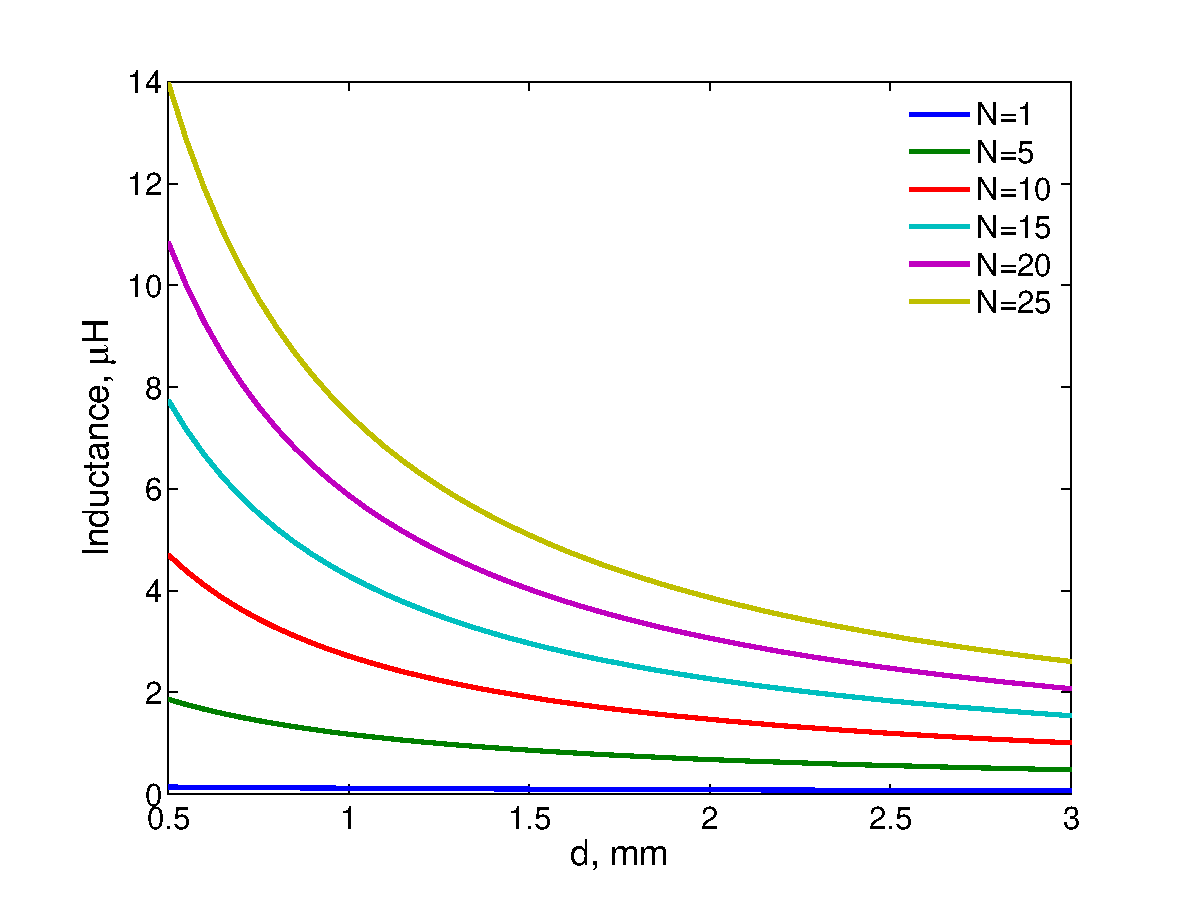
\includegraphics[width=0.6\textwidth]{./images/Lvsd}
\caption{Inductance w.r.t. wire diameter for fixed coil radius of 4 cm and different turns}
\label{F:Lvsd}
\end{center}
\end{figure}

Due to commercial availability we select two different wire diameter, displayed in the following table:

\begin{table}[h]
\begin{center}
\begin{tabular}{|c|c|c|}

\noalign{\global\arrayrulewidth1pt}
\hline
\textbf{Wire diameter} 	& 	\textbf{Insulation} & 	\textbf{Total diameter}\\
\hline
\hline
1 mm		& Polymeric varnish & 	$\sim{}${1 mm}		\\ \hline 
0.59 mm 	& Polymeric layer	& 	1.4 mm 				\\ \hline

\end{tabular}
\caption{Wire diameter}
\label{T:varnish}
\end{center}
\end{table}








				\subsubsection{Number of turns}
First, we determine the maximum number of turns for the quad-copter in 20 turns. This number did not compromise the drone stability in its vertical axis because does not change at all the gravity center. Having a wire reference maximum diameter of 1.4 mm, it means that the largest coil of 20 turns will have 2.8 cm of height, even less height than the quadcopter.

\begin{figure}[htb]
\begin{center}
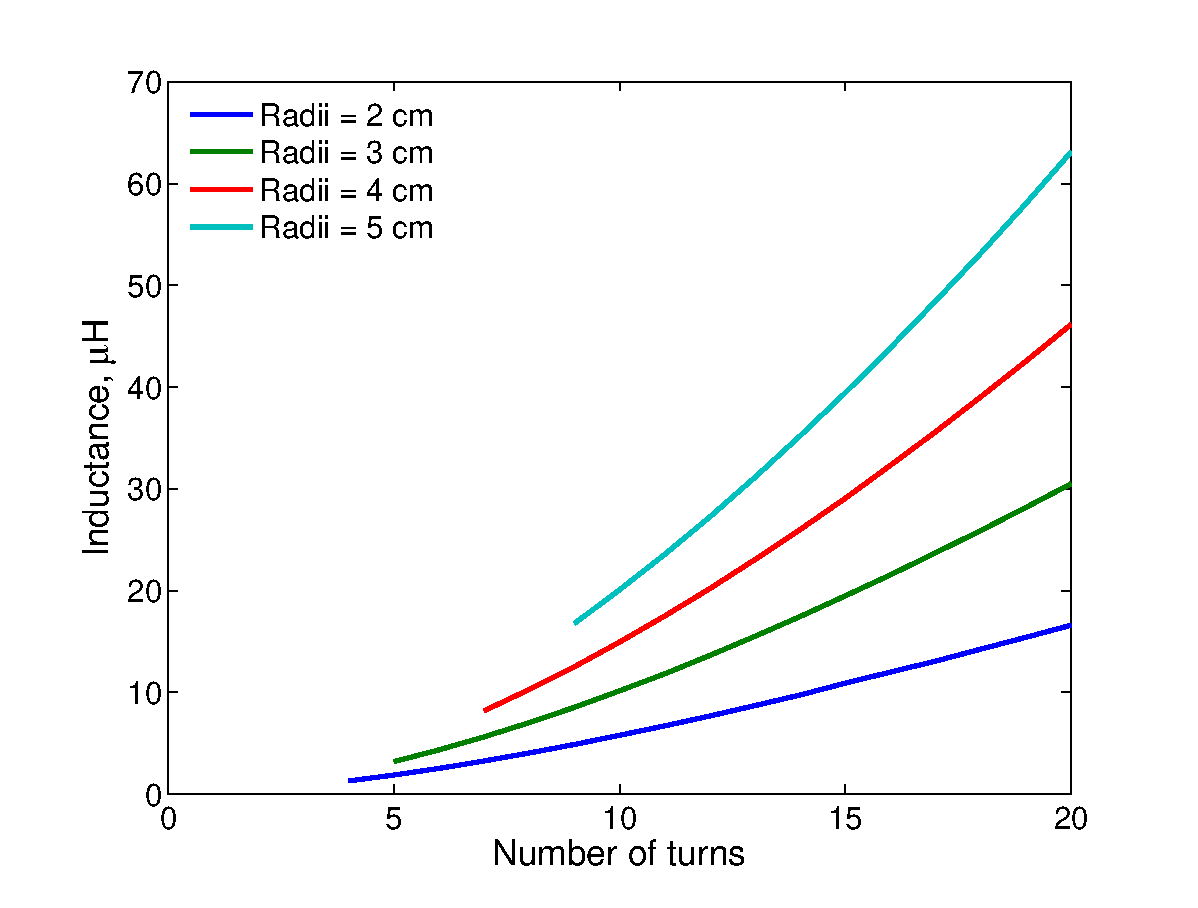
\includegraphics[width=0.6\textwidth]{./images/LvsN}
\caption{Calculated inductance for different number of turns and coil radii values}
\label{F:LvsN}
\end{center}
\end{figure}

Figure \ref{F:LvsN} shows coil inductance depending on the number of turns and on the radius. As the number of turns is increased, coil inductance rises proportionally. In addition, for the same number of turns, higher inductance values are obtained whether the coil radius is increased. It is observed that plotted lines tend to move to the right. This effect is caused by the interpolation method used in this graph, which does not provide higher $D/h$ values from the reference table \cite{WaiKaiChen}. Initially, an increase in coil's radius appears to improve the quality factor of the coil which is a desired purpose. Regrettably we are again in a trade-off situation. By increasing the number of turns we are also increasing the total wire length. This results in a lower quality factor knowing that it is inversely proportional to coil resistance (Equation \ref{eq:Qfactor}). It must be mentioned here that coupling factor does not depend on the number of turns.









				\subsubsection{Coil radius}\label{subsec:geo} %\subsection{Geometrical constraints}
As we said in \ref{sec:discussion}, midrange WPT applications contain distances from coil diameter up to ten times the coil diameter. Thus, if we aspire to transfer power up to 20 cm, at least, a coil with 2 cm of diameter is needed. To design such a smaller coil was refused because it involved imprecise winding, and obviously the smaller the coil area, the smaller magnetic flux is created (\ref{flux}). On the contrary, a great area will imply to have an unbalanced drone which is not designed for carrying oversized objects. The increase in coil area probably will turn into an overall weight-gain.

Furthermore, it has been studied the relation between \textit{Tx} and \textit{Rx} coil area. An axial distance between coils several times the coil radius implies a very small coupling factor $k$ which can be around 0.01 \cite{lowCouplingFactor}. Taking into account that coupling factor lies between 0 and 1, this low value means that only a small amount of the flux generated by \textit{Tx} coil links the \textit{Rx} coil. 

The dashed line set in 0.05 m on the vertical axis means the maximum \textit{Tx} radius allowable owing to the nano-quadcopter dimensions.

\begin{figure}[htb]
\begin{center}
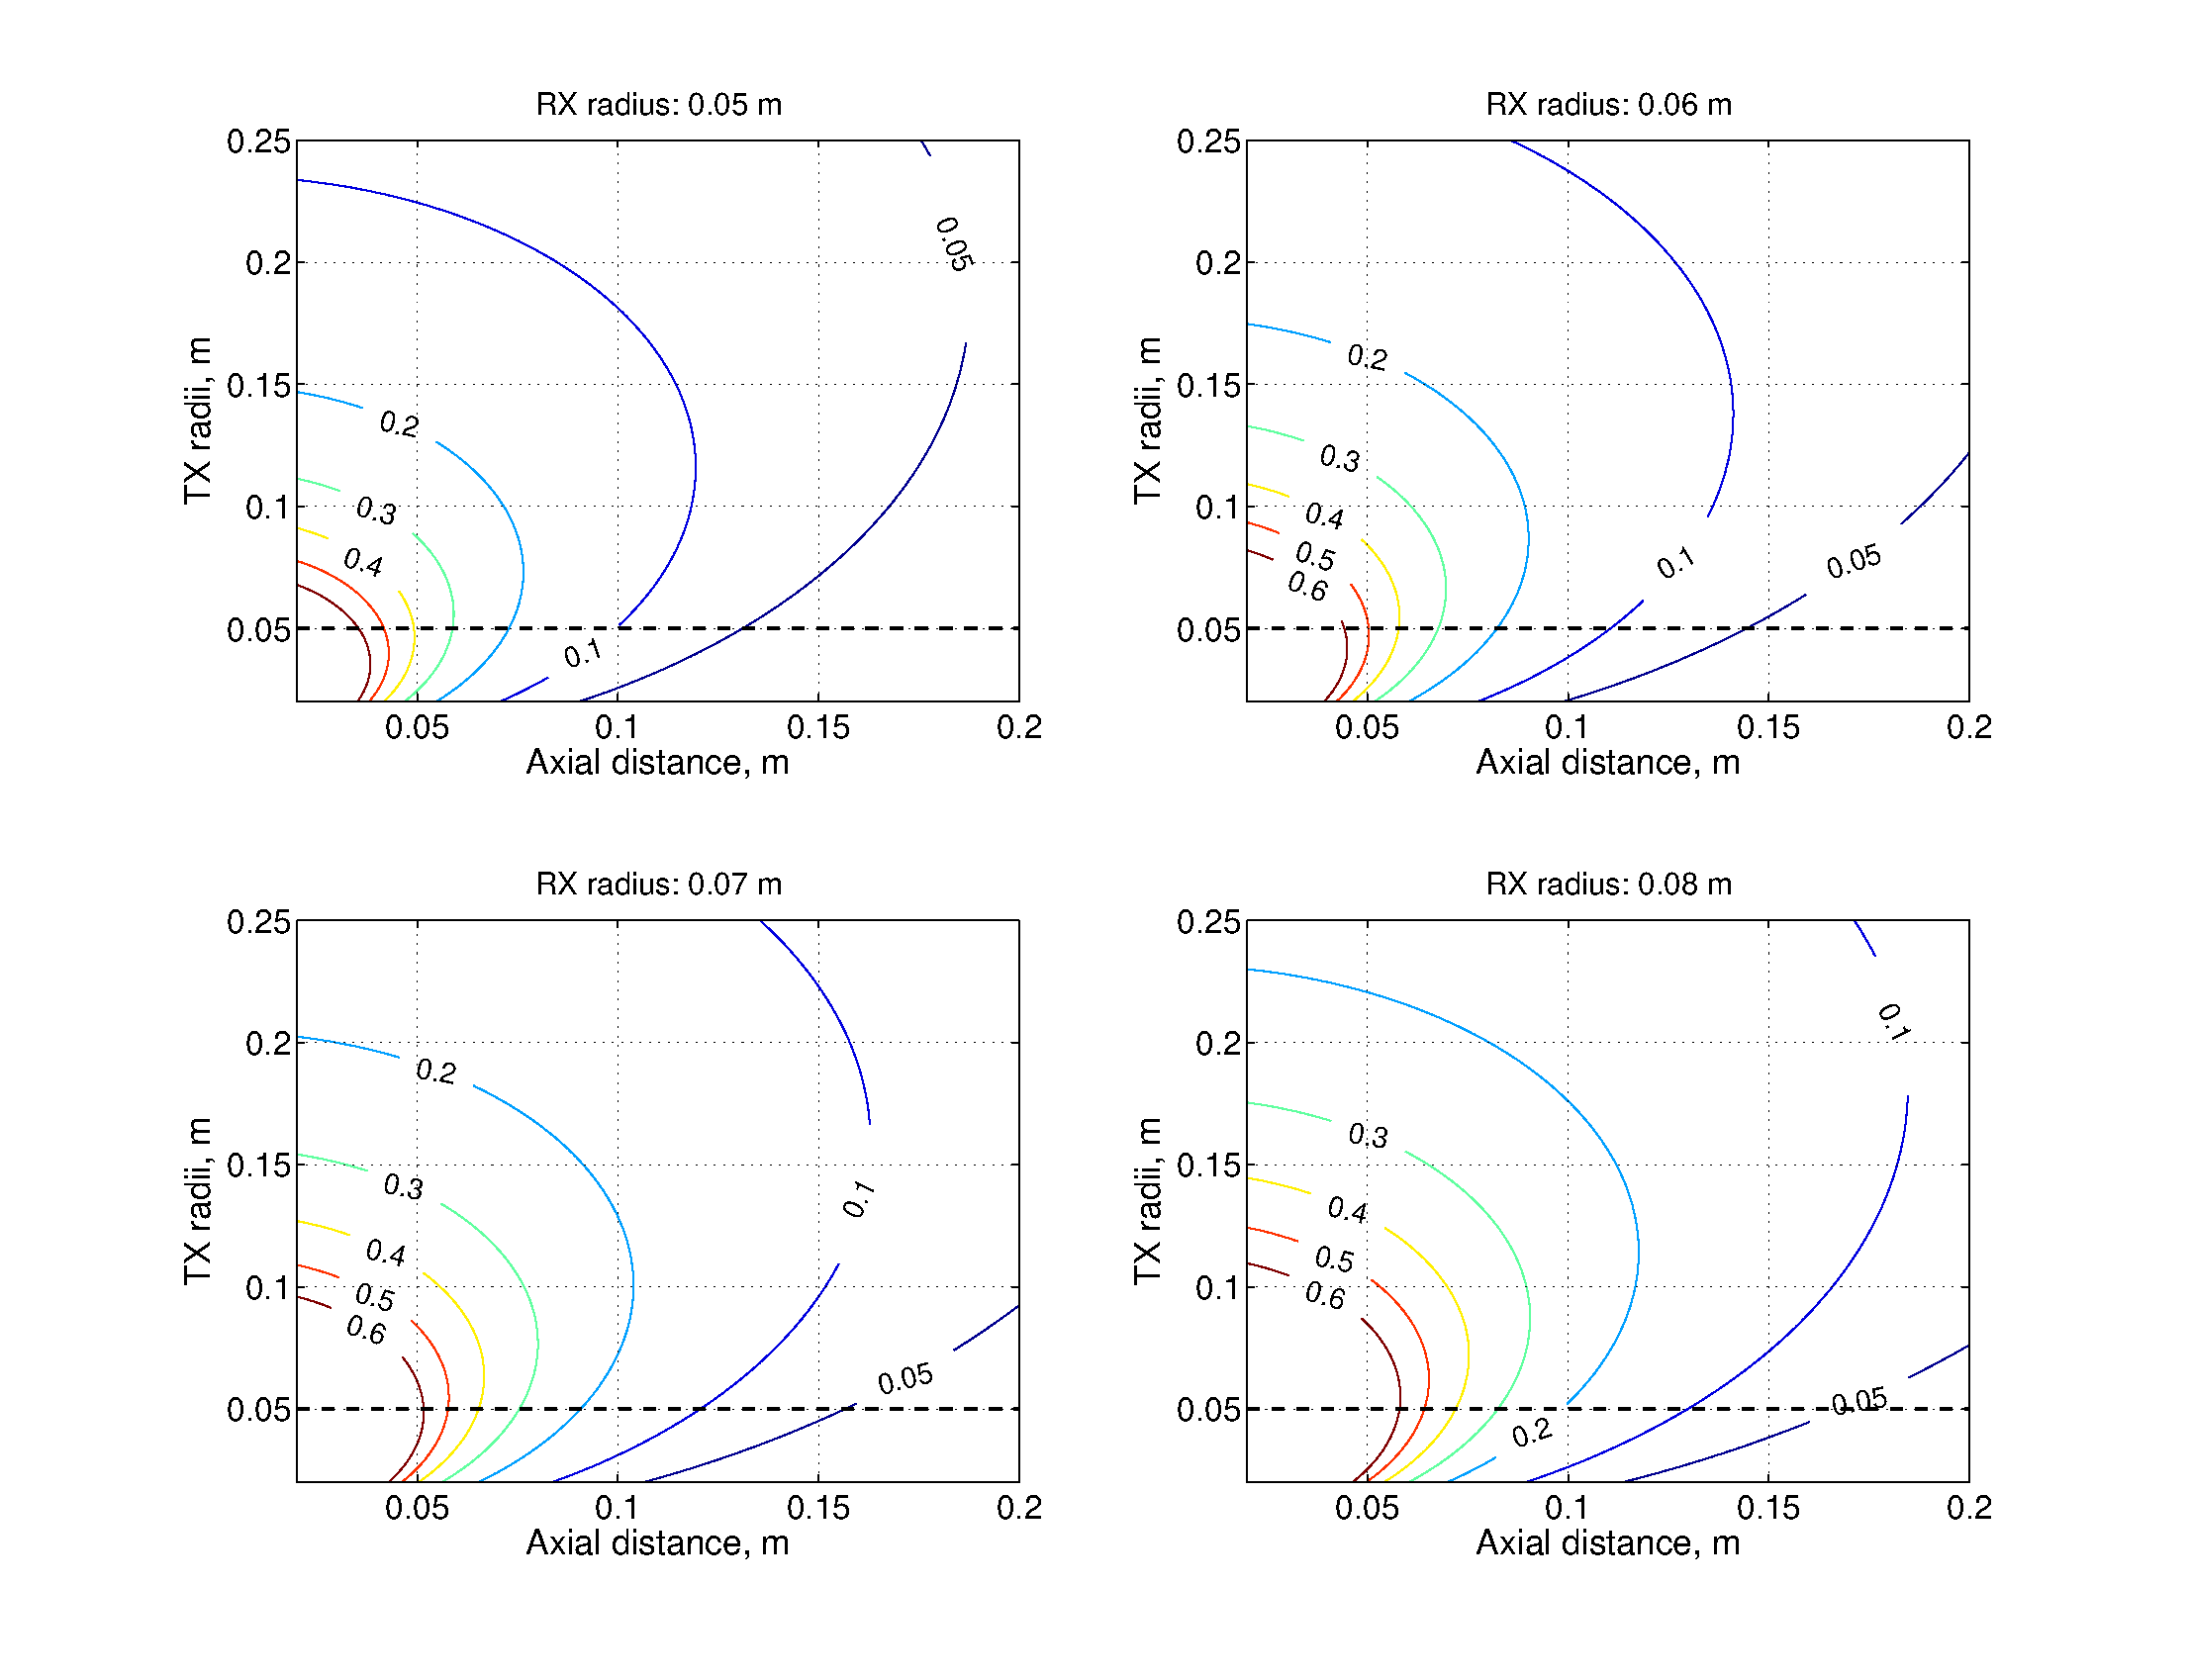
\includegraphics[width=1\textwidth]{./images/contourLines2}
\caption{Contour lines of the magnetic coupling obtained for different distances}
\label{F:contourLines}
\end{center}
\end{figure}

Contrary to common assumption, for larger air gaps the maximum of the magnetic coupling $k$ can not be reached with coils of equal size \cite{7_Optimized_Magnetic_Design}. Figure \ref{F:contourLines} shows the contour lines of the magnetic coupling factor for different air distances and transmitter coil radii for four receiver coil radii. In this case, it has been used the Equation \ref{Eq:typical} to calculate inductances.

It can be shown that bigger \textit{Rx} coils radii improve the coupling factor between the coils, meanwhile increasing \textit{Tx} coil radius does not involve achieving higher $k$ factor. This can be seen with the following example; for a given air gap distance, $z = 0.1$ m, and a fixed \textit{Rx} radius, $R_{RX} = 0.05$ m, by increasing \textit{Rx} radius in 3 cm we see that the coupling factor doubles its value from 0.1 to 0.2. However much \textit{Tx} radius is increased, it will never be possible to duplicate $k$ for the chosen axial distance.  
		
			\subsubsection{Weight} % by default
The \textit{Crazyflie 2.0} 4 DC-motors give it a maximum take-off weight of 42 g \cite{crazyflie}. Part of this payload must be reserved for the transmission circuit and coil's outfitting supports, so we decide to set the coil mass in about 12 g. It must be said that this limitation only affects to the transmitter side.

% Taking into account that this nano quadcopter weighs 27g its maximum payload is set on 15g. 



%%%%%%%%%%%%%%%%%%%%%%%%%%%%
%%%   					 %%%
%%%   Candidate Models   %%%
%%% 					 %%%
%%%%%%%%%%%%%%%%%%%%%%%%%%%%

		\section{Detailed Designs}\label{finTFG}
With intent to create completely different coils we decided to maximize both the coil area and the number of turns while fixing the other variables. The coil shape was round because of its benefits when creating a magnetic field. A copper wire was chosen for its low electrical resistance, as it was said previously. 

% Three coils were designed using the algorithm shown in Figure \ref{F:coilAlgorithm}. The algorithm was initially thought for a 1 mm wire diameter. It maximizes the coil weight in order to take advantage of the quadcopter performance. This results in two completely different coil designs. The first prioritizes the largest possible radius and so few turns. The second model is designed with the minimum radius, which is defined in subsection \ref{subsec:geo}, and the maximum turns permitted. A third model was created in order to test a mixture model. These ``candidates" will allow us to discern clearly the difference between coils' behaviour.

Three coils were designed using the algorithm shown in Figure \ref{F:coilAlgorithm}. The algorithm is thought for a 1 mm copper wire diameter. It maximizes the coil weight in order to take advantage of the quadcopter performance. This results in two completely different coil designs. Note that all coil possibilities have the same or similar lengths. The first model prioritizes the largest possible radius and so few turns. The second is designed with the minimum radius, which is defined in subsection \ref{subsec:geo}, and the maximum turns permitted. A third model was created in order to test a trade-off model. These ``candidates" will allow us to discern clearly the difference between coils' behaviour.

\begin{table}[ht]
\begin{center}
\begin{tabular}{cccccc}

\noalign{\global\arrayrulewidth1pt}
\hline
\noalign{\global\arrayrulewidth0.4pt}
\textbf{Model name} 	& \textbf{Turns} 	& 	\textbf{Radius} & 	\textbf{Wire diameter} & 	$\bm{D/h}$ \textbf{ratio} & 	\textbf{Tx mass}\\
\noalign{\global\arrayrulewidth1pt}
\hline
\noalign{\global\arrayrulewidth0.4pt}
Model A  & 8 	& 	5 cm 	& 	0.597 mm 	& 	11.9 &	13.4 g\\ \hline 
Model B  & 19 	& 	2 cm 	& 	0.597 mm 	& 	1.5  & 	14.1 g\\ \hline 
Model C  & 10 	& 	4 cm 	& 	0.597 mm 	& 	5.71 & 	13.5 g\\ \hline 
Model D1 & 7 	& 	4 cm 	& 	1 mm 		& 	8    & 	17.3 g\\ \hline 
Model D2 & 11 	& 	1.5 cm  & 	1 mm 		& 	2.73 & 	9.8 g\\ \hline 

\end{tabular}
\caption{Geometric parameters of coil models}
\label{T:coil Models}
\end{center}
\end{table}

Both \textit{Tx} and Rx coils were designed with the same dimensions for each of the models A, B and C. This assumption simplifies future computations and also provides us with an added ease for the coil winding procedure. Anyway, we build the last two single-models $D1$ and $D2$ in order to demonstrate the theoretical calculations, which state that an increment in \textit{Rx} radius is preferred upon the same increment in \textit{Tx} radius. 

All the experimental results are carried out for wire of 1.4 mm of diameter, but including its covering (0.59 mm without covering). In this manner we take into account the increase in mass because of the thermal epoxy adhesive inclusion. The wire diameter reduction does not affect since it does still not surpass the boundary stated skin depth, $d>5\delta$. Thus, we ensure not to surpass the maximum payload after adding the adhesive fixation, using a ``lighter'' wire owing to a reduction in the cross-sectional area. In addition, the parasitic capacitance of the coil is reduced due to wire plastic layers, and therefore more space between wires.



% While producing the coils we realized that copper coils of 1 mm of diameter exceeded in mass because of the thermal epoxy adhesive inclusion. Therefore, all the experimental results are carried out for wire of 1 mm of diameter, but now including its covering (0.59 mm without covering). This reduction does not affect since it does still not surpass the boundary stated skin depth, $d>5\delta$. Thus, we ensure not to surpass the maximum payload using a ``lighter'' coil owing to a reduction in the cross-sectional area. In addition we reduce the parasitic capacitance of the coil because of the inclusion of plastic layers, and therefore more space between wires.
% \hfill \break
\begin{figure}[H]

\begin{center}
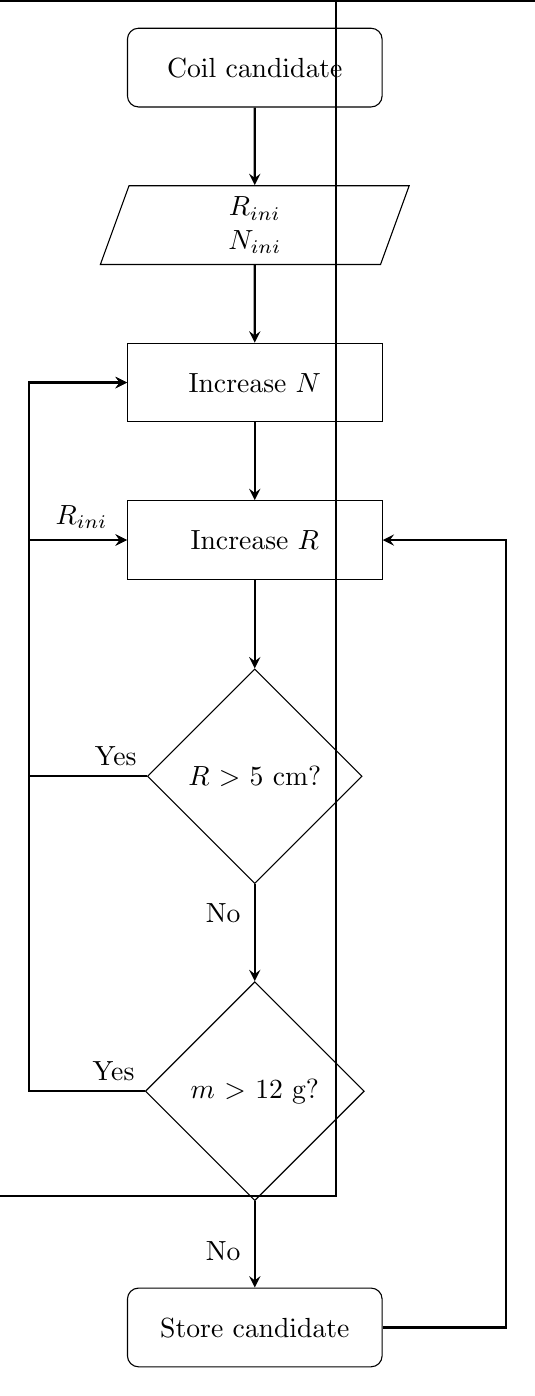
\begin{tikzpicture}[node distance=2cm]
\vspace{-2em}
	% Define labels
	\node (start) [startstop] {Coil candidate};
	\node (in1) [io, below of=start] {$R_{ini}$\\$N_{ini}$};
	\node (pro1) [process, below of=in1] {Increase $N$};
	\node (pro2) [process, below of=pro1] {Increase $R$};
	\node (dec1) [decision, below of=pro2, yshift=-1.0cm] {$R>$ 5 cm?};
	\node (dec2) [decision, below of=dec1, yshift=-2.0cm] {$m>$ 12 g?};
	\node (end) [startstop, below of=dec2, yshift=-1.0cm] {Store candidate};
	
	% Locate weird labels
	% \node [label={[shift={(-2.2,-4.1)}]$R_{ini}$}] {};
	\node [label={[shift={(-2.2,-6.1)}]$R_{ini}$}] {};
	\node [label={[shift={(-0.4,-11.1)}]No}] {};
	\node [label={[shift={(-0.4,-15.4)}]No}] {};

	% Draw vertical arrows
	\draw [arrow] (start) -- (in1);
	\draw [arrow] (in1) -- (pro1);
	\draw [arrow] (pro1) -- (pro2);
	\draw [arrow] (pro2) -- (dec1);
	\draw [arrow] (dec1) -- (dec2);
	\draw [arrow] (dec2) -- (end);

	% Draw weird arrows
	\draw [arrow] (dec1.west) node[above left]   {Yes} -- + (-15mm,0) |- (pro1.west);
	\draw [arrow] (dec1.west) node[above left]   {} -- + (-15mm,0) |- (pro2.west);
	\draw [arrow] (dec2.west) node[above left]   {} -- + (-14.65mm,0) |- (pro1.west);
	\draw [arrow] (dec2.west) node[above left]   {Yes} -- + (-14.65mm,0) |- (pro2.west);
	\draw [arrow] (end.east) node[above right]   {} -- + (+15.65mm,0) |- (pro2.east);
	% \draw [arrow] (end.east) node[above right]   {} -- + (+15.65mm,0) |- (pro1.east);

\end{tikzpicture}
\end{center}
\caption{Flowchart of the algorithm to design the coil size}
\label{F:coilAlgorithm}
\end{figure}


		\subsection{Discussion}
The decision of which coil model will be outfitted on the quadcopter is based on two criteria: performance and stability. Performance is related with the ability of transfer energy from the source to the load, and so the power transferred and the efficiency. In spite of the fact that the performance has been studied in detail selecting the best compensation topology, in this project the main goal is intended to transfer power, hence the efficiency will not be a decisive parameter.

The second and not less important criteria has to do with weight and shape. Having all the models similar weight it will be determinant to see how does each model behaves, together with the quadcopter. 

It will be necessary to wait until experimental tests to decide which coil is the most suitable. Then, according to the chosen model, it will be set one or other operating frequency.

In Chapter \ref{C:experimental}, all models are tested and compared with theoretical results. It will also be demonstrated that model C is the most appropriate model for transferring power. 

% , we opt for model C for being the most adequate in shape and for working in conjunction with the quadcopter. Model A has a radius too small for landing maneuvers. On the contrary, model B has a radius bigger than the quadcopter complicating the coil support. 




% \begin{table}[ht]
% \centering
% \begin{tabular}{|c|c|c|c|c|c|}

% \noalign{\global\arrayrulewidth1pt}
% \hline
% \textbf{Model name}  &   \textbf{Inductance} 	&   \textbf{Resistance} 	&   \textbf{Q factor} 	&   \textbf{Capacitor}  \\
% \hline
% \hline
% % \tablefootnote{The low inductance and resistance values of model A are due to weight restriction. Model A is a 23\% shorter than other models. By winding one turn involved to exceed mass constraint. Bigger diameters required more adhesive fixation.}

% Model A 	& 7.62$\mu$H 	& 0.489$\Omega$   & 	97 		& 31 nF     \\ \hline 
% Model B  	& 12.72$\mu$H 	& 0.619$\Omega$   & 	129 	& 31 nF 	\\ \hline
% Model C 	& 13.26$\mu$H 	& 0.651$\Omega$   & 	127 	& 31 nF 	\\ \hline

% \end{tabular}
% \caption{Theoretical coil calculations for a test frequency of 1 MHz}
% \label{T:theoretical}
% \end{table}

 




\chapter{Architecture and Design of the WPT System} \label{C:architecture}
Once the inductive coupling system has been studied in detail, it is time to outfit the selected coil model C on the drone. The selection of this model is argued in Chapter \ref{C:experimental}, after all the measures are performed. In this chapter, the required circuits to design the WPT system are discussed. In the first section, the nano-quadcopter used is introduced and all its main features are explained, as well as the necessity of designing brand new motor mounts in order to support the coil. 

In the second part of the chapter, the architecture of the transmitter and receiver circuits is explained, as well as its design. The main feature of the WPT system lies on energy conversion. Hence, both the transmitter and the receiver circuits need of power converters. As shown in Figure \ref{F:blockDiagram} the transmitter includes a ultra low DC-DC converter and a DC-AC converter. At the receiving side, the power converters include at least an AC-DC converter. Later, for the used application, a DC-DC converter will be introduced for the battery recharging circuit.

%%%
%%%
%%% SE ESCOGE LA BOBINA C !!! EXPLICAR QUE TODO EL CAPITULO SE TIENE EN CUENTA
%%%
%%%

\begin{figure}[htb]
\begin{center}
\vspace{+0.5em}
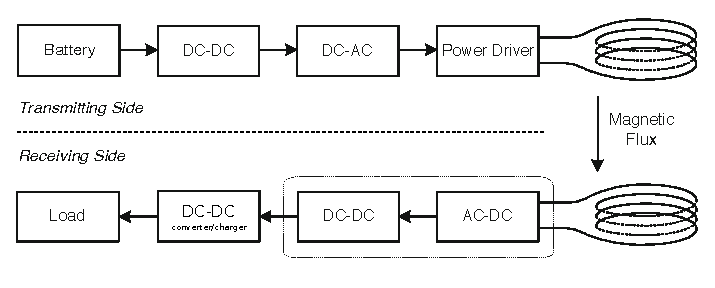
\includegraphics[width=0.9\textwidth]{./images/block2}
% \vspace{-1.5em}
\caption{Block diagram}
\label{F:blockDiagram}
\end{center}
\end{figure}


  \section{Quadcopter}
One of the initial objectives of the project is the WPT system outfitting on the nano-quadcopter. The inclusion of the quadcopter as an energy \textit{transporter} restricts both transmitter and receiver side, but mainly the transmitter because of the weight. The model used in this work is the created by \textit{Bitcraze}, its second nano-quadcopter version, named \textit{Crazyflie 2.0}. 

The assembly of this quadcopter can be divided into two parts. The first is composed by the battery, motors and headers attaching. In the second, the propellers are introduced and balanced. This last procedure is really important due the fact that well balanced propellers reduce vibrations in the copter and noise in the sensors improving the stability of the \textit{Crazyflie}.


\begin{figure}[H]
\centering
\begin{subfigmatrix}{2}
\vspace{1em} 
\hspace*{\fill}%
\subfigure[Crazyflie 2.0] 
  {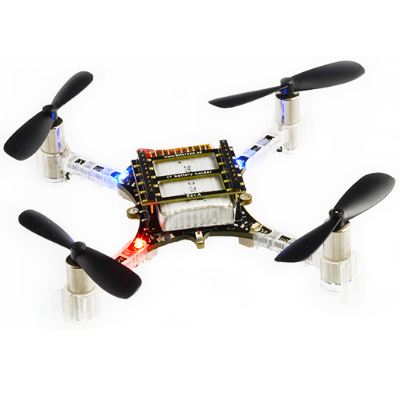
\includegraphics[width=2.2in]{./images/crazyflie}}\hfill 
\subfigure[CrazyRadio USB dongle]
  {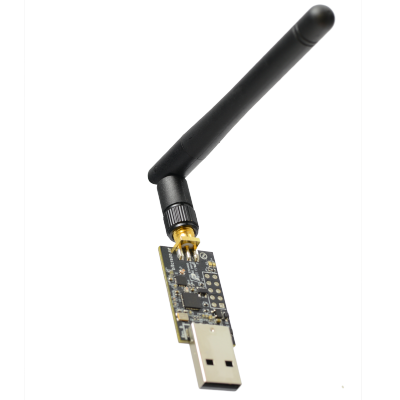
\includegraphics[width=2.0in]{./images/CrazyRadio}}
\hspace*{\fill}%
\end{subfigmatrix}
\caption{Transmitter circuit}
% \label{F:transmitter}
\end{figure}

Contrary to other drones, \textit{Crazyflie} allowed us the possibility to fly it indoor. It also has many interesting features listed in Table \ref{F:crazyflieFeatures} which made us to select it. Owing to the fact that \textit{Crazyflie} is an open source project it is possible to log, graph and set variables in real-time via the USB radio dongle.

\begin{figure}[htb]
\begin{center}
\begin{tabular}{|c|c|}

  \hline
  \multicolumn{2}{|c|}{\bf{Crazyflie 2.0 specification}} \\
  \hline
  \hline
  Size (WxHxD)  & 92x92x29 mm \\ \hline
  \multirow{2}{*}{Radio specs} 
   &  Low energy Bluetooth\\
   &  Radio amplifier 1 km range \\ \hline
  \multirow{3}{*}{Controllers} 
   &  STM32F405 MCU\\
   &  $\mu$USB connector \\
   &  USB OTG capability \\ \hline
  \multirow{3}{*}{IMU} 
   &  3 axis gyro \\
   &  3 axis accelerometer \\
   &  3 axis magnetometer \\
   &  Pressure sensor \\
  \hline

\end{tabular}
\caption{Crazyflie 2.0 features}
\label{F:crazyflieFeatures}
\end{center}
\end{figure}


    \subsection{Controlling the \textit{Crazyflie}}
As it is shown in Table \ref{F:crazyflieFeatures}, the \textit{Crazyflie} can be either controlled by a mobile device or a computer. Using a mobile device is the fastest way to control it, but its maneuverability is reduced compared to the computer option. Therefore, this last one is chosen.

The two needed requirements for flying the \textit{Crazyflie} using a computer are: a radio USB dongle (\textit{Crazyflie PA}) for communication and a standard gamepad for maneuvering. In addition, a virtualization program is required to run the \textit{Crazyflie} client. Few drivers are needed, as well as the last updated software in order to avoid any \textit{bug}. Both drivers and the needed code are uploaded on \textit{GitHub} repositories \cite{github}. 

\begin{figure}[H]
\centering
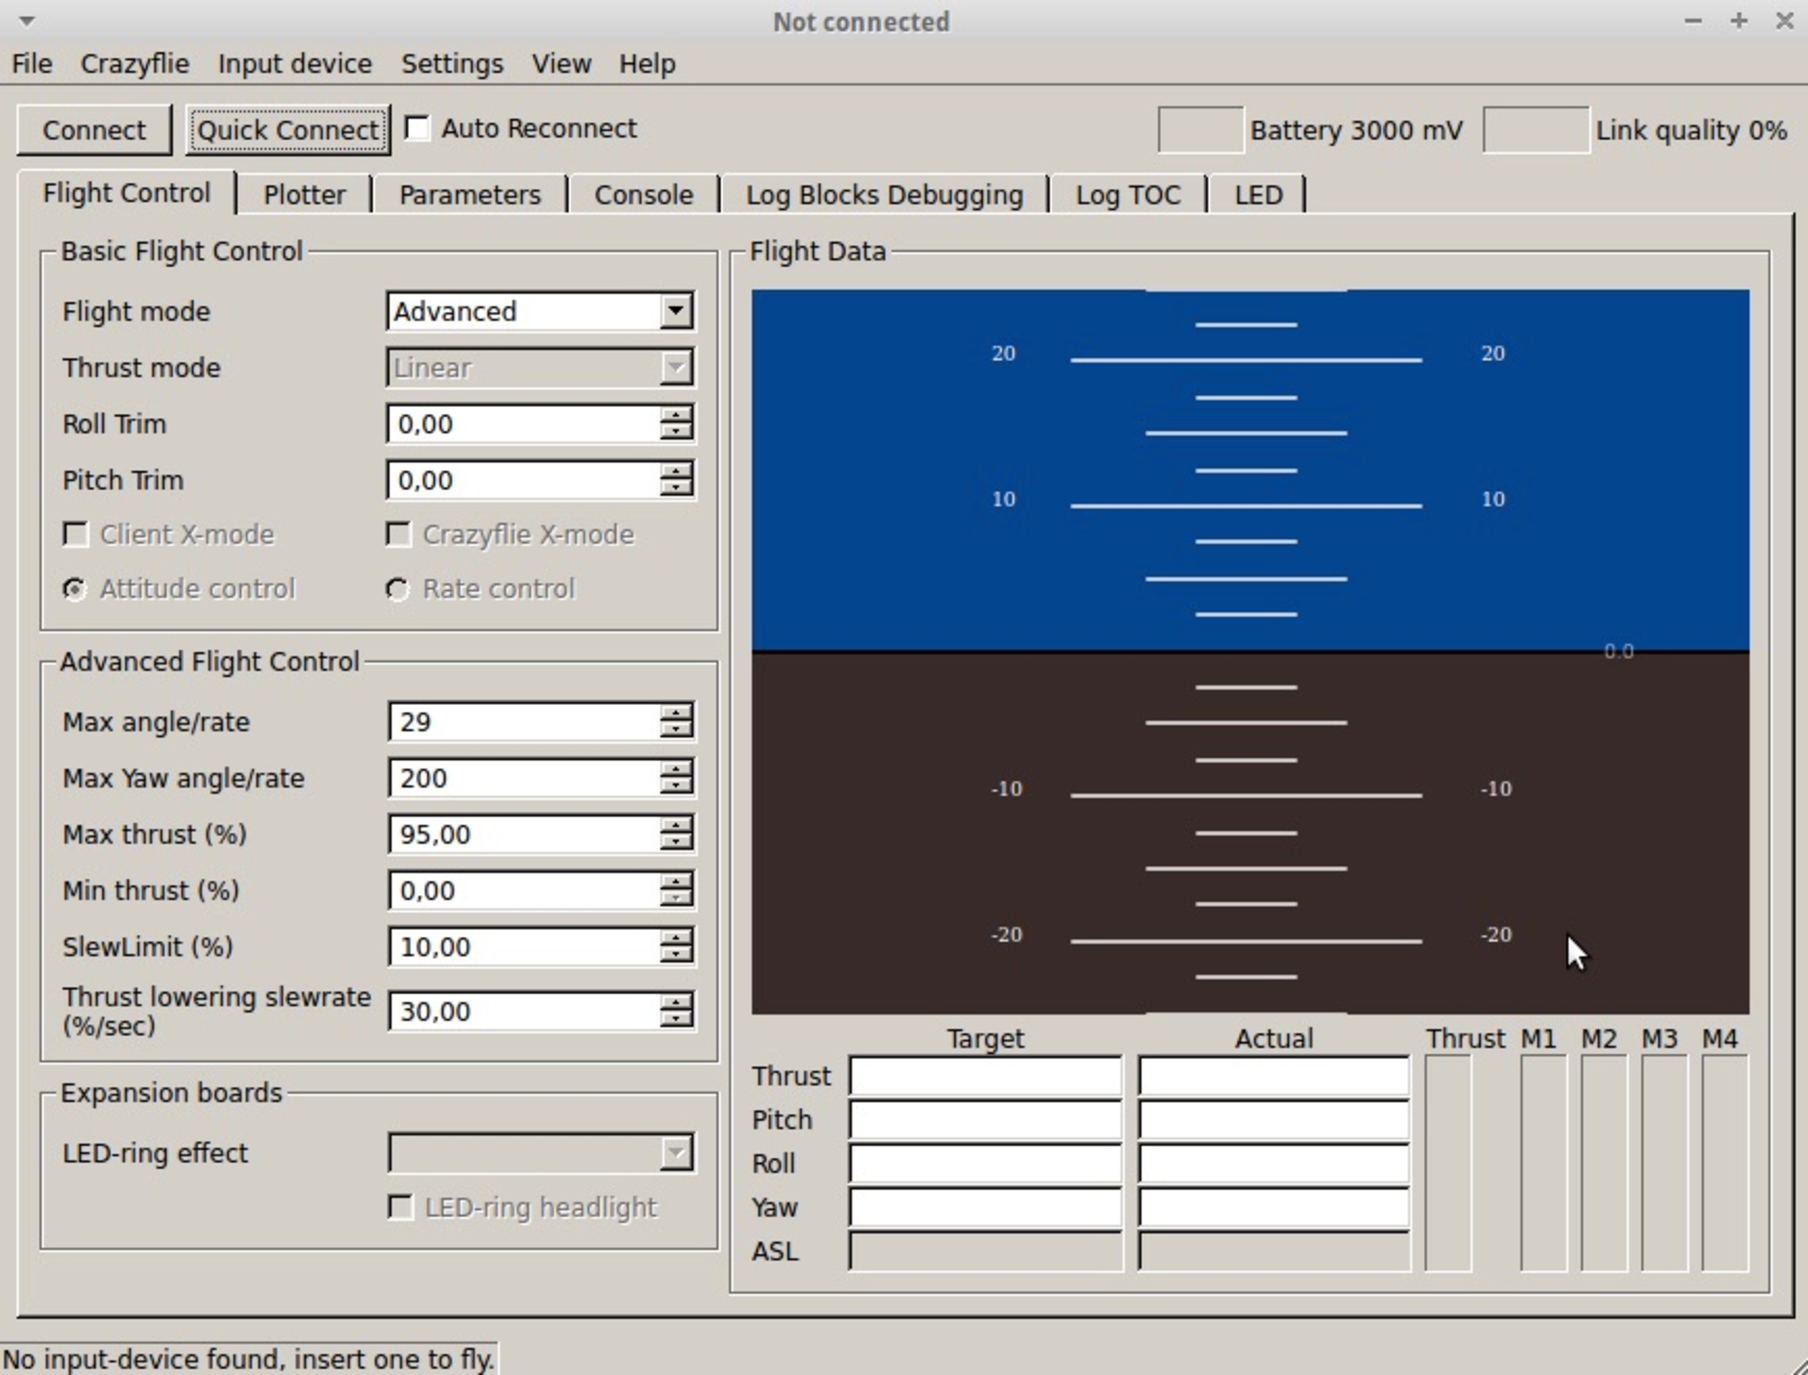
\includegraphics[width=0.65\textwidth]{./images/virtual}
\caption{Crazyflie's computer client}
\end{figure}


  \subsection{Motor Mount Design}

With the original design of the \textit{Crazyflie} nano-quadcopter is almost impossible to install it the used coil. As a consequence, in this case, the coil would not be subjected neither precisely, nor ``smartly''. The solution is to redesign the motor mounts of the \textit{Crazyflie} to accomplish a good coil support.

Using the CAD software \textit{SolidWorks}, it has been designed a motor mount with the same characteristics of the original mounts. The only difference is that the designed structure is made to place the coil under the \textit{Crazyflie}. 


This structure has the main characteristic of supporting lateral stresses, as the \textit{default} mounts, and also to prevent the fall of the coil, by using a kind of hook placed at the end of the mount arm. The complete design schematics are located in the Appendices. All this mentioned characteristics are showed in Figures \ref{F:MM} and \ref{F:MMC}. 

\begin{figure}[H]
\centering
\begin{subfigmatrix}{3} 
\subfigure[Plan and elevation views] 
  {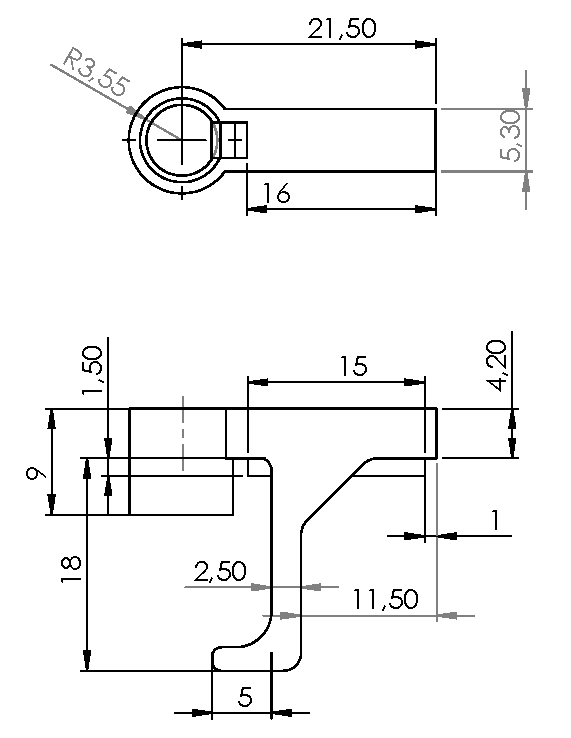
\includegraphics{./images/plantaAlzado}\label{F:MM}}
\subfigure[3D model] 
  {\includegraphics{./images/3dmount}\label{F:MMC}}
\subfigure[Real view image]
  {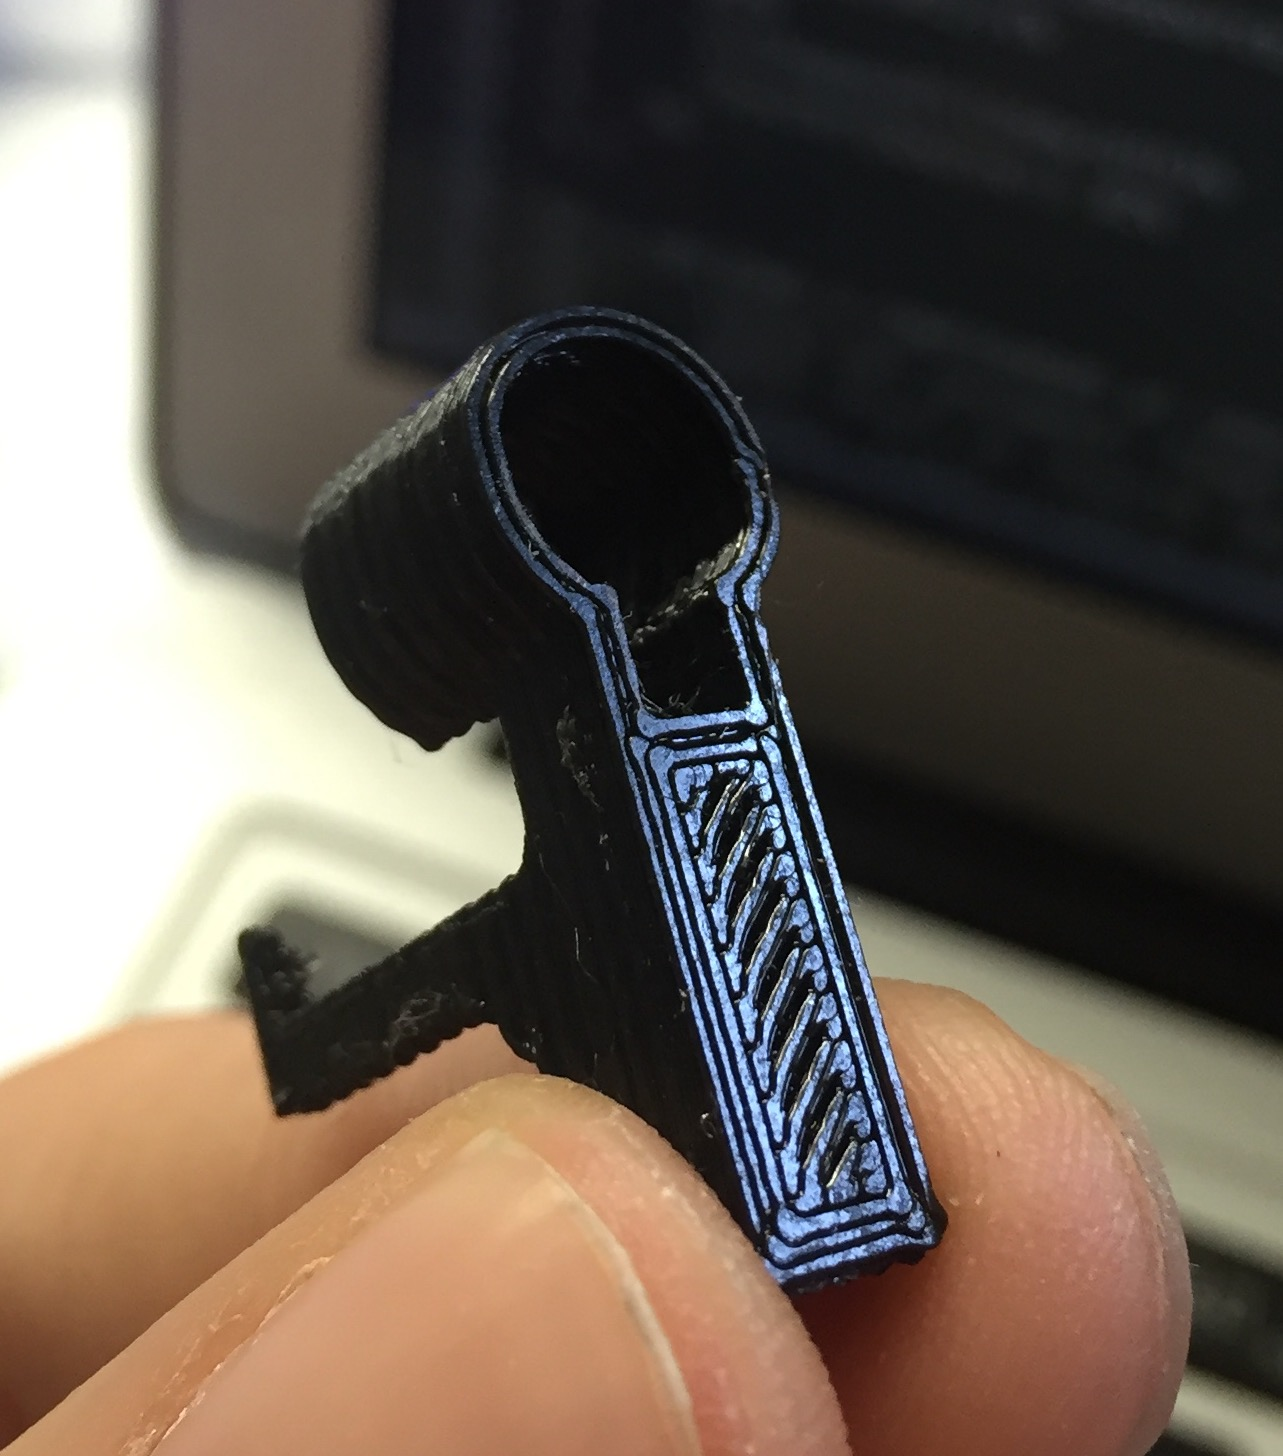
\includegraphics{./images/FullSizeRender}\label{F:finalMount}}
\end{subfigmatrix}
\caption{Motor mount process design}
\end{figure}

Once the motor mount is designed it can be printed with a 3D printer. The result is exhibited in Figure \ref{F:finalMount}.



  \section{Transmission System}

In a WPT system, the transmitter is intended for carrying power in order to satisfy the receiver demand. Its design is based on two premises; size and weight. Size is important in order to maintain the nano-quadcopter balanced owing to \textit{Crazyflie} is not designed to carry objects. The weight constraint is repeated several times during this project.

% Therefore, weight is the parameter which will define transmission subsystems.

    \subsection{Power Source}
After considering different options, such as using two isolated batteries for feeding the drone and the induction system separately, we decided to use the default battery of the nano-quadcopter, and so avoiding to increase the total weight. The battery \textit{Crazyflie} uses is of the type LiPo (Lithium-Polymer).
    
\begin{figure}[htb]
\begin{center}
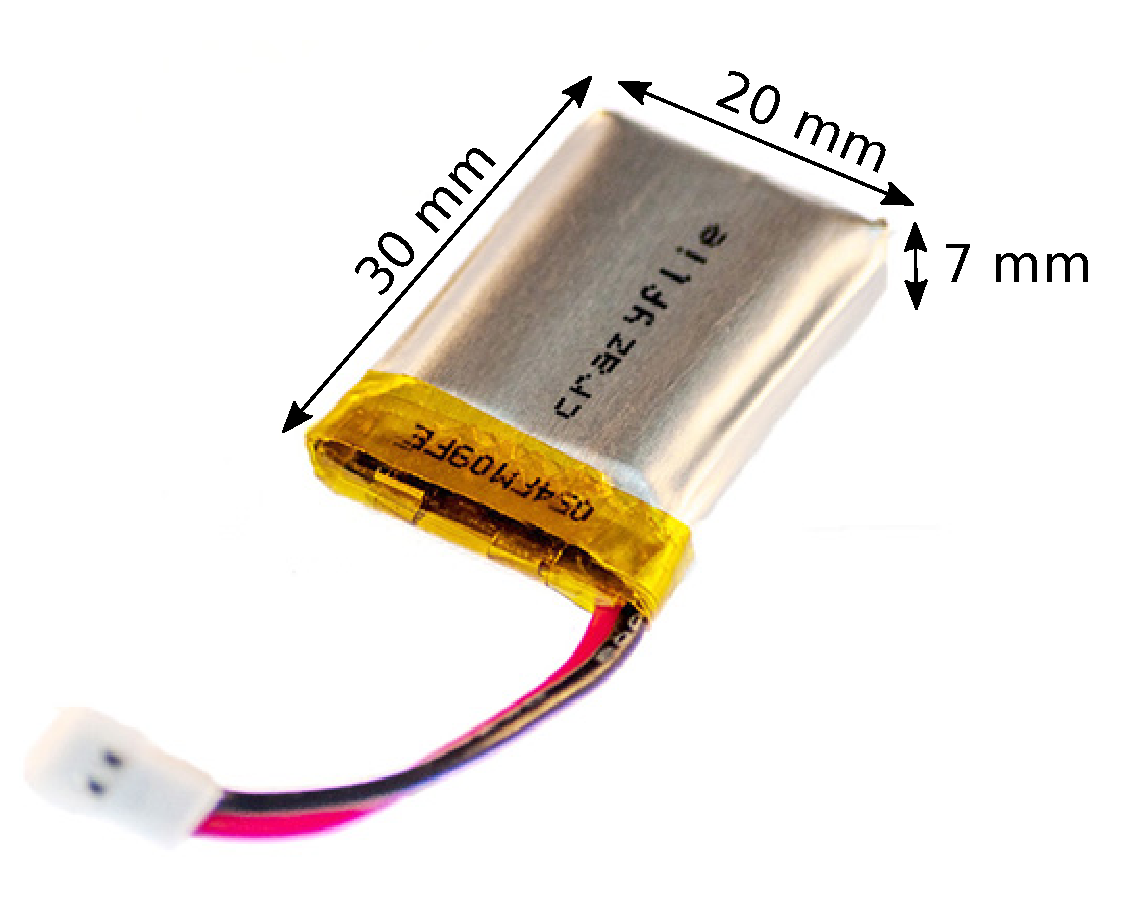
\includegraphics[width=0.4\textwidth]{./images/battery}
\caption{Crazyflie's battery size}
\label{F:battery}
\end{center}
\end{figure}

Althought LiPo is not the safest chemistry, these batteries are currently the most popular type for radiocontrol use. The reason is due to LiPo batteries has the best power to weight ratios and discharge currents. It also allows to use only a single cell.


\begin{table}[ht]
\begin{center}
\begin{tabular}{|c|c|c|c|}

\noalign{\global\arrayrulewidth1pt}
\hline
\textbf{Capacity}  &   \textbf{Nominal voltage}   &   \textbf{Discharge}    &   \textbf{Charge}\\
\hline
\hline
240 mAh   & 3.7 V   &   15C   &   2C  \\ \hline 

\end{tabular}
\caption{Battery's electrical specifications}
\label{T:batterySpecs}
\end{center}
\end{table}

The electrochemical batteries have the advantage over other energy storage devices, such as supercapacitors, that their main discharge curve is exponential, meaning that the energy stays high during most of the charge and then drops rapidly as the charge depletes \cite{batteryDischarge}. The \textit{Crazyflie} battery discharge rate or C-rate is of 15C which means 15-times the rated capacity.

As it is stated in \cite{crazyflie}, the maximum flight time with LiPo battery is up to 7 minutes. Theoretically with motors at full power and consuming 3600 mA, the flight is being reduced to 4 minutes. Regrettably, this time will be even reduced by the inclusion of the induction system. 

The end-of-discharge voltage for most LiPo is 3.0 V/cell. At this level, roughly 95 percent of the energy is spent and the voltage would drop rapidly if the discharge were to continue \cite{batteryDischarge}. To protect the battery from over-discharging, which is very sensitive to, the quadcopter comes with a PCM (Protection Circuit Module) that prevents operation beyond a specified end-of-discharge voltage. 










\subsection{Voltage Regulator}
The voltage regulator was the last system implementation. Owing to the necessity of having 12 V, explained in Chapter \ref{C:experimental}, on the transistor collector, a switching voltage regulator is the most appropriate solution. Linear regulators can only step down the input voltage and the possibility of adding a second battery was rejected because of weight. 

Switching regulators are highly efficient and able to boost, buck and invert voltages with ease, but they also have weaknesses. One of them is that they are complex chips and, consequently, it can take a lot of design effort to get a new product working properly. In addition, the level of integration of contemporary switching regulators does not come cheaply and increases the chip size \cite{regulators}.

To solve these issues the \textit{Webench} application is used. This design tool developed by \textit{Texas Instruments} allows to design the voltage regulator that better adjusts to our input and output power requirements. 

\begin{table}[htb]
\begin{center}
\begin{tabular}{|c|c|c|}

\noalign{\global\arrayrulewidth1pt}
\hline
\textbf{Input Voltage}  &   \textbf{Output Voltage}   &   \bf{Output Current}\\
\hline
\hline
3 - 3.7 V       & 12 V   &   0.5 A  \\ \hline 

\end{tabular}
\caption{Regulator requirements}
\label{T:regulator}
\end{center}
\end{table}

\begin{figure}[H]
  \begin{center}
    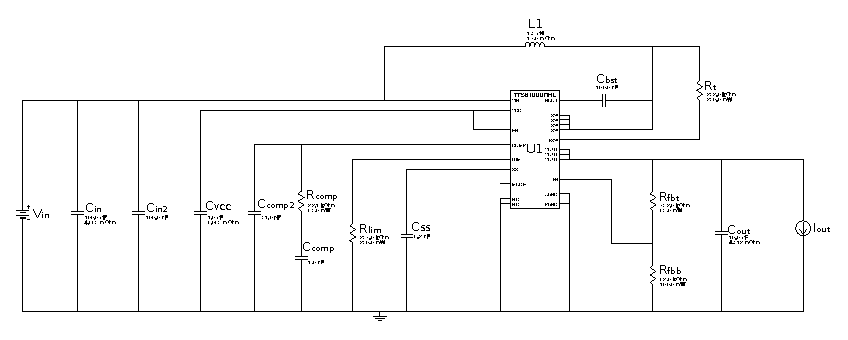
\includegraphics[width=1.05\textwidth]{./images/TPS61088}
  \caption{TPS61088 design circuit}
  \end{center}
\end{figure}

It must be said that the regulator is designed to provide a maximum output current of 500 mA, which is the maximum input current of the power driver, discussed later.

The requirements above lead us to different switching regulators. By looking at size and efficiency, the TPS 61088 was the one with best efficiency per unit of area. The circuit schematic is given in Appendix \ref{Appendix: DC-DC}.

Although an ideal switcher has a $100\%$ efficiency, the actual efficiency is about $92\%$ (Appendix \ref{Appendix: DC-DC}) and it depends on the output current and the input voltage. The power \textit{lost} is really low and it is dissipated following,

\begin{equation}
P_{dis} = \left(\frac{1}{\eta}-1\right)\cdot{P{out}}
\end{equation}


The input current that the regulator is drawing to the battery can be calculated using Equation \ref{eq:regulator}, and it defines the global circuit consumption. 

\begin{equation}\label{eq:regulator}
I_{in} = \left({I_{out}}\cdot\frac{V_{out}}{V_{in}}\right)/{\eta}
\end{equation}

Before computing $I_{in}$, it will be necessary to figure out which is the output current and which relies on the power driver. 









    \subsection{Oscillator} 
A Quartz Crystal Oscillator (XO) is used to generate the necessary periodic signal which generates the alternating current in the \textit{Tx} coil. It is selected for its good performance, a low power consumption, and a simple electronic circuit. This type of oscillator not only provides an extraordinary frequency stability, but it also provides a constant frequency output under varying load conditions, which is an important aspect to consider.

\begin{figure}[H]
\begin{center}
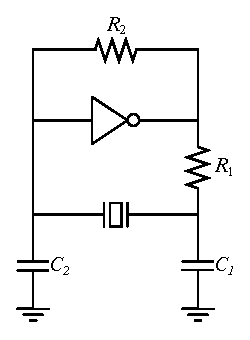
\includegraphics[width=0.3\textwidth]{./images/oscilador}
\caption{Oscillator schematic}
\label{F:oscillator}
\end{center}
\end{figure}

The functioning of the quartz crystal oscillator is based on piezoelectric effect. Piezoelectricity is the primary property of a crystal which makes it usable as resonator. Piezoelectricity is a reversible property of a crystal by which an electrical charge produces a mechanical force by changing the shape of the crystal and vice versa, a mechanical force applied to the crystal produces an electrical charge \cite{quartzCrystal}. 

As it is discussed at the end of the previous chapter, each coil model has its own resonant frequency, and therefore a unique oscillator circuit. For the selected coil model, the resonant frequency is 0.95 MHz. 

The characteristic frequency of the crystal, or rate of vibration, is determined by the cut, size, and shape of the quartz crystal. Therefore, to achieve the desired frequency of 0.95 MHz a special crystal is needed. Hence, taking advantage on the wide Q factor of coils, an standard crystal frequency of 1 MHz is selected. 

\begin{table}[htb]
\begin{center}
\begin{tabular}{|c|c|}

\noalign{\global\arrayrulewidth1pt}
\hline
\textbf{Parameter}  &   \textbf{Value}\\
\hline
\hline
Frequency       & 1 MHz                  \\ \hline 
$R_1$           & 9.1 M$\Omega$          \\ \hline 
$R_2$           & 910 $\Omega$           \\ \hline 
$C_1$           & 47 pF                \\ \hline
$C_2$           & 47 pF                \\ \hline  
Consumption     & 8.4 mA                 \\ \hline

\end{tabular}
\caption{XO parameters}
\label{T:XOparameters}
\end{center}
\end{table}


In figure above, it is represented the Pierce oscillator circuit. This parallel oscillator is a derivative of the Colpitts oscillator. The circuit is implemented using a minimum of components: a single CMOS inverter gate, two resistors, two capacitors and the quartz crystal.

For high speed CMOS logic families, typically \cite{oscilador}:
\begin{itemize}[noitemsep] % To be more compact --> \begin{itemize}[noitemsep,nolistsep]
  \item $R_1$ is between 8.2 M$\Omega$ and 10 M$\Omega$
  \item $R_2$ is between 470 $\Omega$ and 2220 $\Omega$
  \item $C_1$ and $C_2$ are of the order of 62 pF 
\end{itemize}









    \subsection{Power Driver}

The output power delivered from the oscillator is not enough to feed the inductor directly. Thus, a Darlington transistor has been placed after the oscillator to elevate the magnetizing current through the primary coil. This increase in the input power will allow the system to transfer power up to larger distances.

The ULN2803A driver is a high-voltage, high-current Darlington transistor array. The device consists of eight NPN Darlington pairs that feature high-voltage outputs with common-cathode clamp diodes for switching inductive loads. Figure \ref{F:transitor} shows a simplified scheme of the power driver. The complete scheme is attached at Appendix \ref{Appendix: powerDriver}.

\begin{figure}[h]
  \begin{center} 
  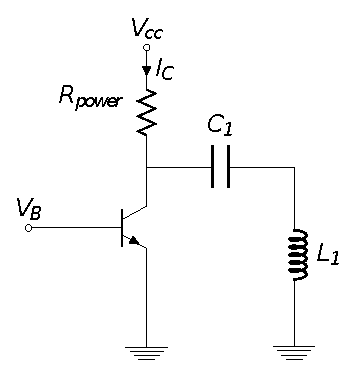
\includegraphics[width=0.4\textwidth]{./images/transistor}
    \caption{Simplified transistor diagram}
    \label{F:transitor}
  \end{center}
\end{figure}

From Figure \ref{F:transitor}, it can be observed that the transistor is working such a switch and driven by the square signal of 0-12 V coming from the oscillator. When an input (pins 1 to 8) is driven ``HIGH'' the corresponding output will switch ``LOW'' sinking current. Likewise, when the input is driven ``LOW'' the corresponding output switches to a high impedance state. This high impedance ``OFF'' state blocks load current and reduces leakage current through the device improving efficiency.

\begin{table}[htb]
\begin{center}
\begin{tabular}{|c|c|}

\noalign{\global\arrayrulewidth1pt}
\hline
\textbf{Parameter}  &   \textbf{Value}\\
\hline
\hline
$V_{CC}$            & 12 V            \\ \hline 
$V_{CE(SAT)}$       & 1.3 V           \\ \hline 
$I_{CC(MAX)}$       & 500 mA          \\ \hline 
$R_{power}$         & 33 $\Omega $      \\ \hline
\end{tabular}
\caption{Electrical characteristics}
\label{T:transistor}
\end{center}
\end{table}


Pin 8 (GND), is connected to the loads ground or 0 volts, while pin 10 ($V_{CC}$) connects to the loads supply. Then any load needs to be connected between +$V_{CC}$ and an output pin, pins 11 to 18. For inductive loads such as coils, pin 10 should always be connected to $V_{CC}$.

The ULN2803A Darlington driver is capable of switching 500 mA per channel. In our case the collector-current $I_{CC}$ is determined using the next expression,

\begin{equation}
I_{CC} = \frac{V_{CC}-V_{CE(SAT)}}{R_{power}}=324\:\textnormal{mA}
\end{equation}

where $R_{power}$ is achieved by combining three resistors in parallel. Each resistor has a resistance value of 100 $\Omega$ and tolerates powers around 1W without any problems. Once the collector current is calculated, it is possible to calculate the total power demanded from the battery. Substituting $I_{CC}$ in equation \ref{eq:regulator} an input current of 1.05 A is obtained. Therefore, the total theoretical power consumed by the transmitter is:

\begin{equation}
P_{in} = V_{in}\cdot{I_{in}}=3.88\:\textnormal{W}
\end{equation} 

It must be also considered the maximum switching frequency of the ULN2803A. Table \ref{T:transistor2} exhibits the propagation delay-times. The most restrictive is the change from ``LOW'' to ``HIGH'' state which takes 130 ns. The delay time delimits a maximum operating frequency of 7.69 MHz. Lowering the operating frequency from this value ensures a better Darlington efficiency.

\begin{table}[htb]
\begin{center}
\begin{tabular}{|c|c|}

\noalign{\global\arrayrulewidth1pt}
\hline
\textbf{Propagation delay time}  &   \textbf{Value}\\
\hline
\hline
 High-Low       & 20 ns           \\ \hline 
 Low-High       & 130 ns          \\ \hline 
\end{tabular}
\caption{Switching characteristics}
\label{T:transistor2}
\end{center}
\end{table}


  \subsection{Transmitter Circuit Assembly}
A printed circuit board (PCB) is needed for physically supporting and wiring the transmitter circuits (regulator, oscillator and power driver). Working with SMD technology makes possible to reduce mostly all the components size. Its round shape is owing to the fact that weight must be distributed as close as possible to the center of gravity. The circular shape also allows to maximize the board space, as well as, not to disturb the coil placement.


\begin{figure}[H]
\centering
\begin{subfigmatrix}{2} 
\hspace*{\fill}
\subfigure[Front view] 
  {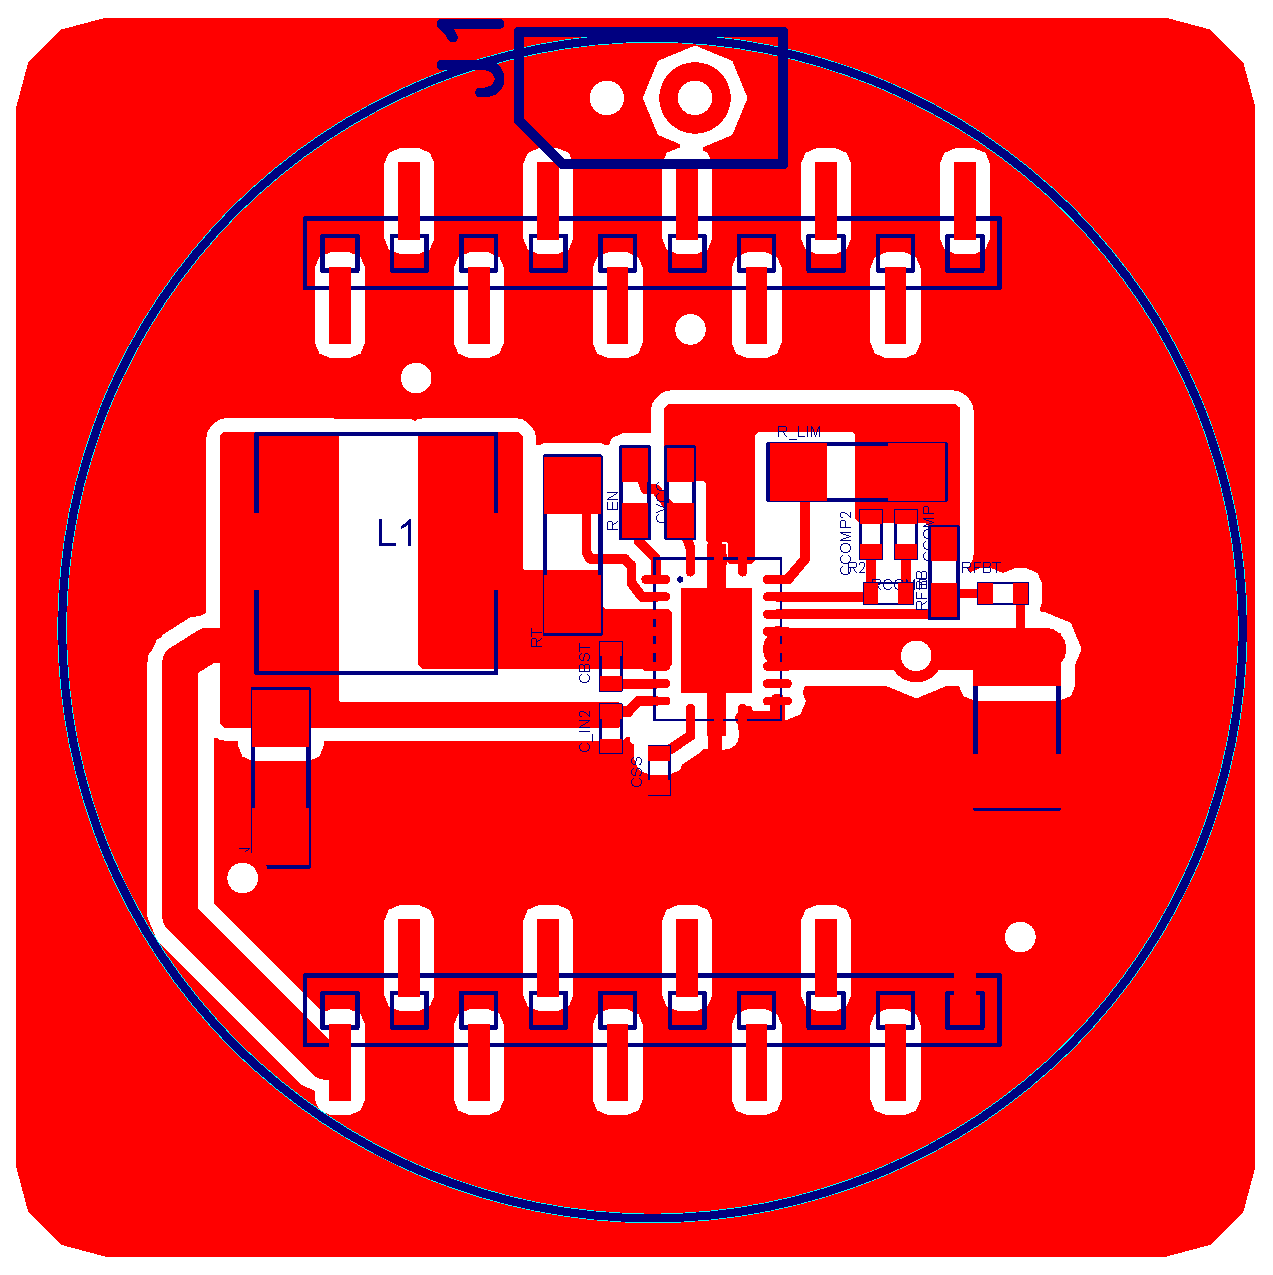
\includegraphics[width=2.0in]{./images/francis1}}\hfill
\subfigure[Back view]
  {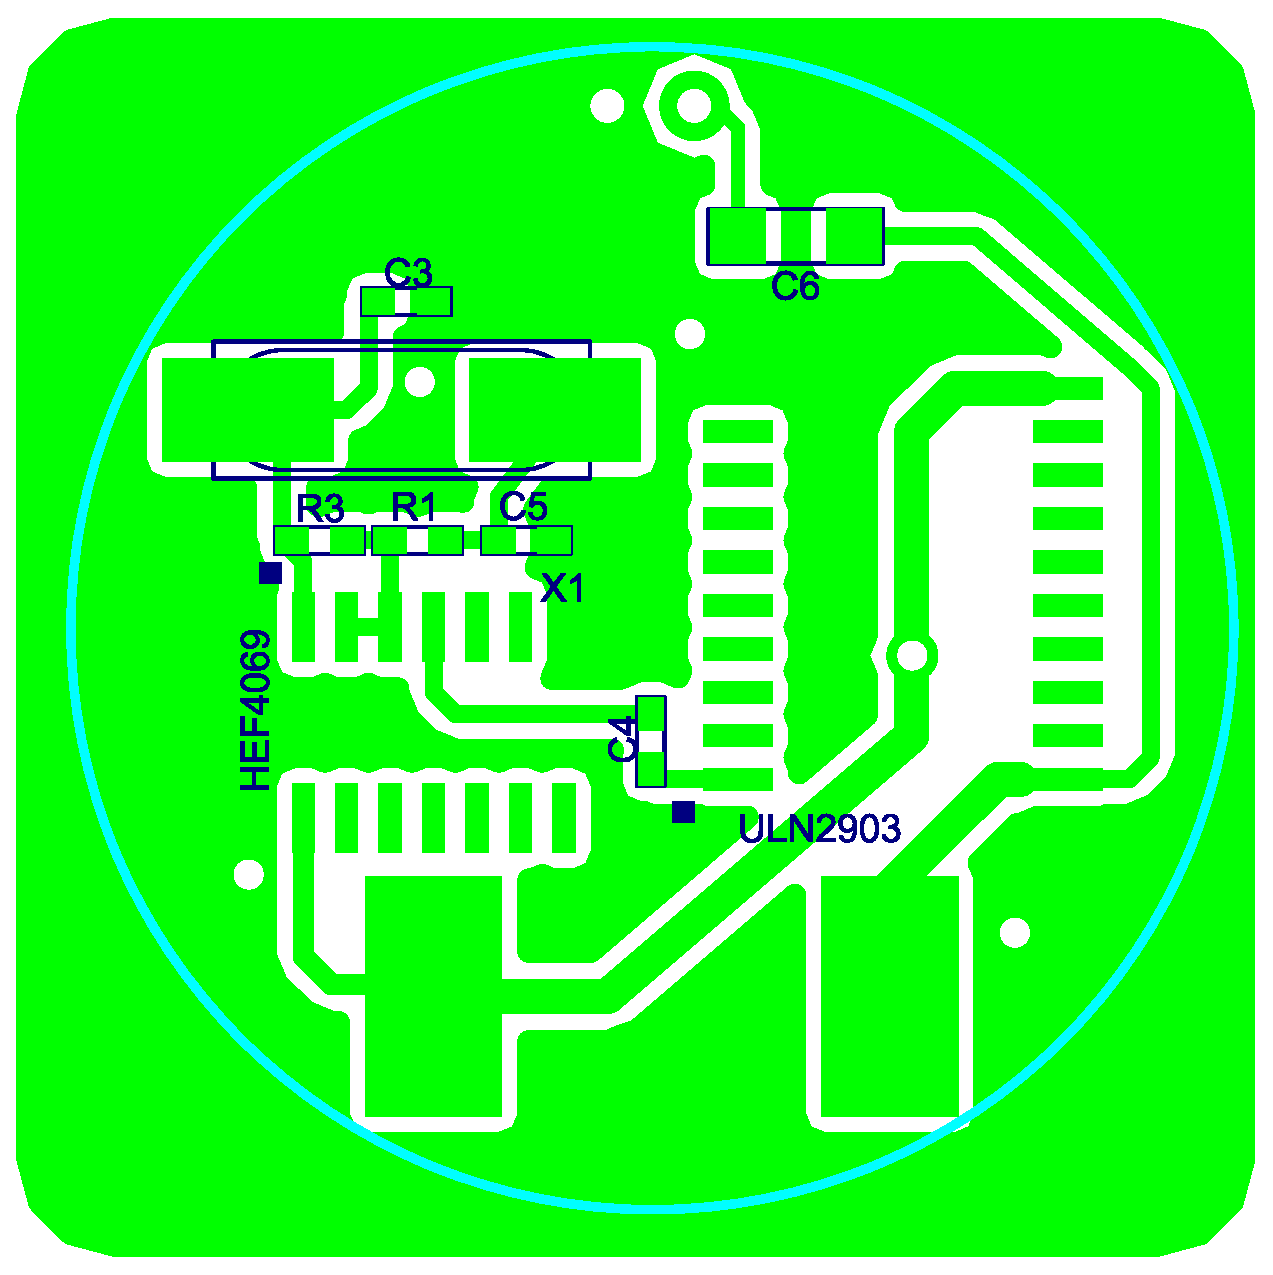
\includegraphics[width=2.0in]{./images/francis2}}
\hspace*{\fill}
\end{subfigmatrix}
\caption{Transmitter SMD design}
\end{figure}

Figure \ref{F:transmitter} exhibits the final transmitter board which is divided in two parts. The top side \ref{F:TX1} is composed by the power driver and the oscillator. It has the input coil pins to attach the primary inductor. The bottom side, invisible when the transmitter is connected to the \textit{Crazyflie}, is formed by the voltage regulator and the adapted pins. Those pins permit to connect directly the board to the quadcopter. The board height is small enough to avoid to graze the floor.


\begin{figure}[H]
\centering
\begin{subfigmatrix}{3}
\vspace{1em} 
\hspace*{\fill}%
\subfigure[Front view] 
  {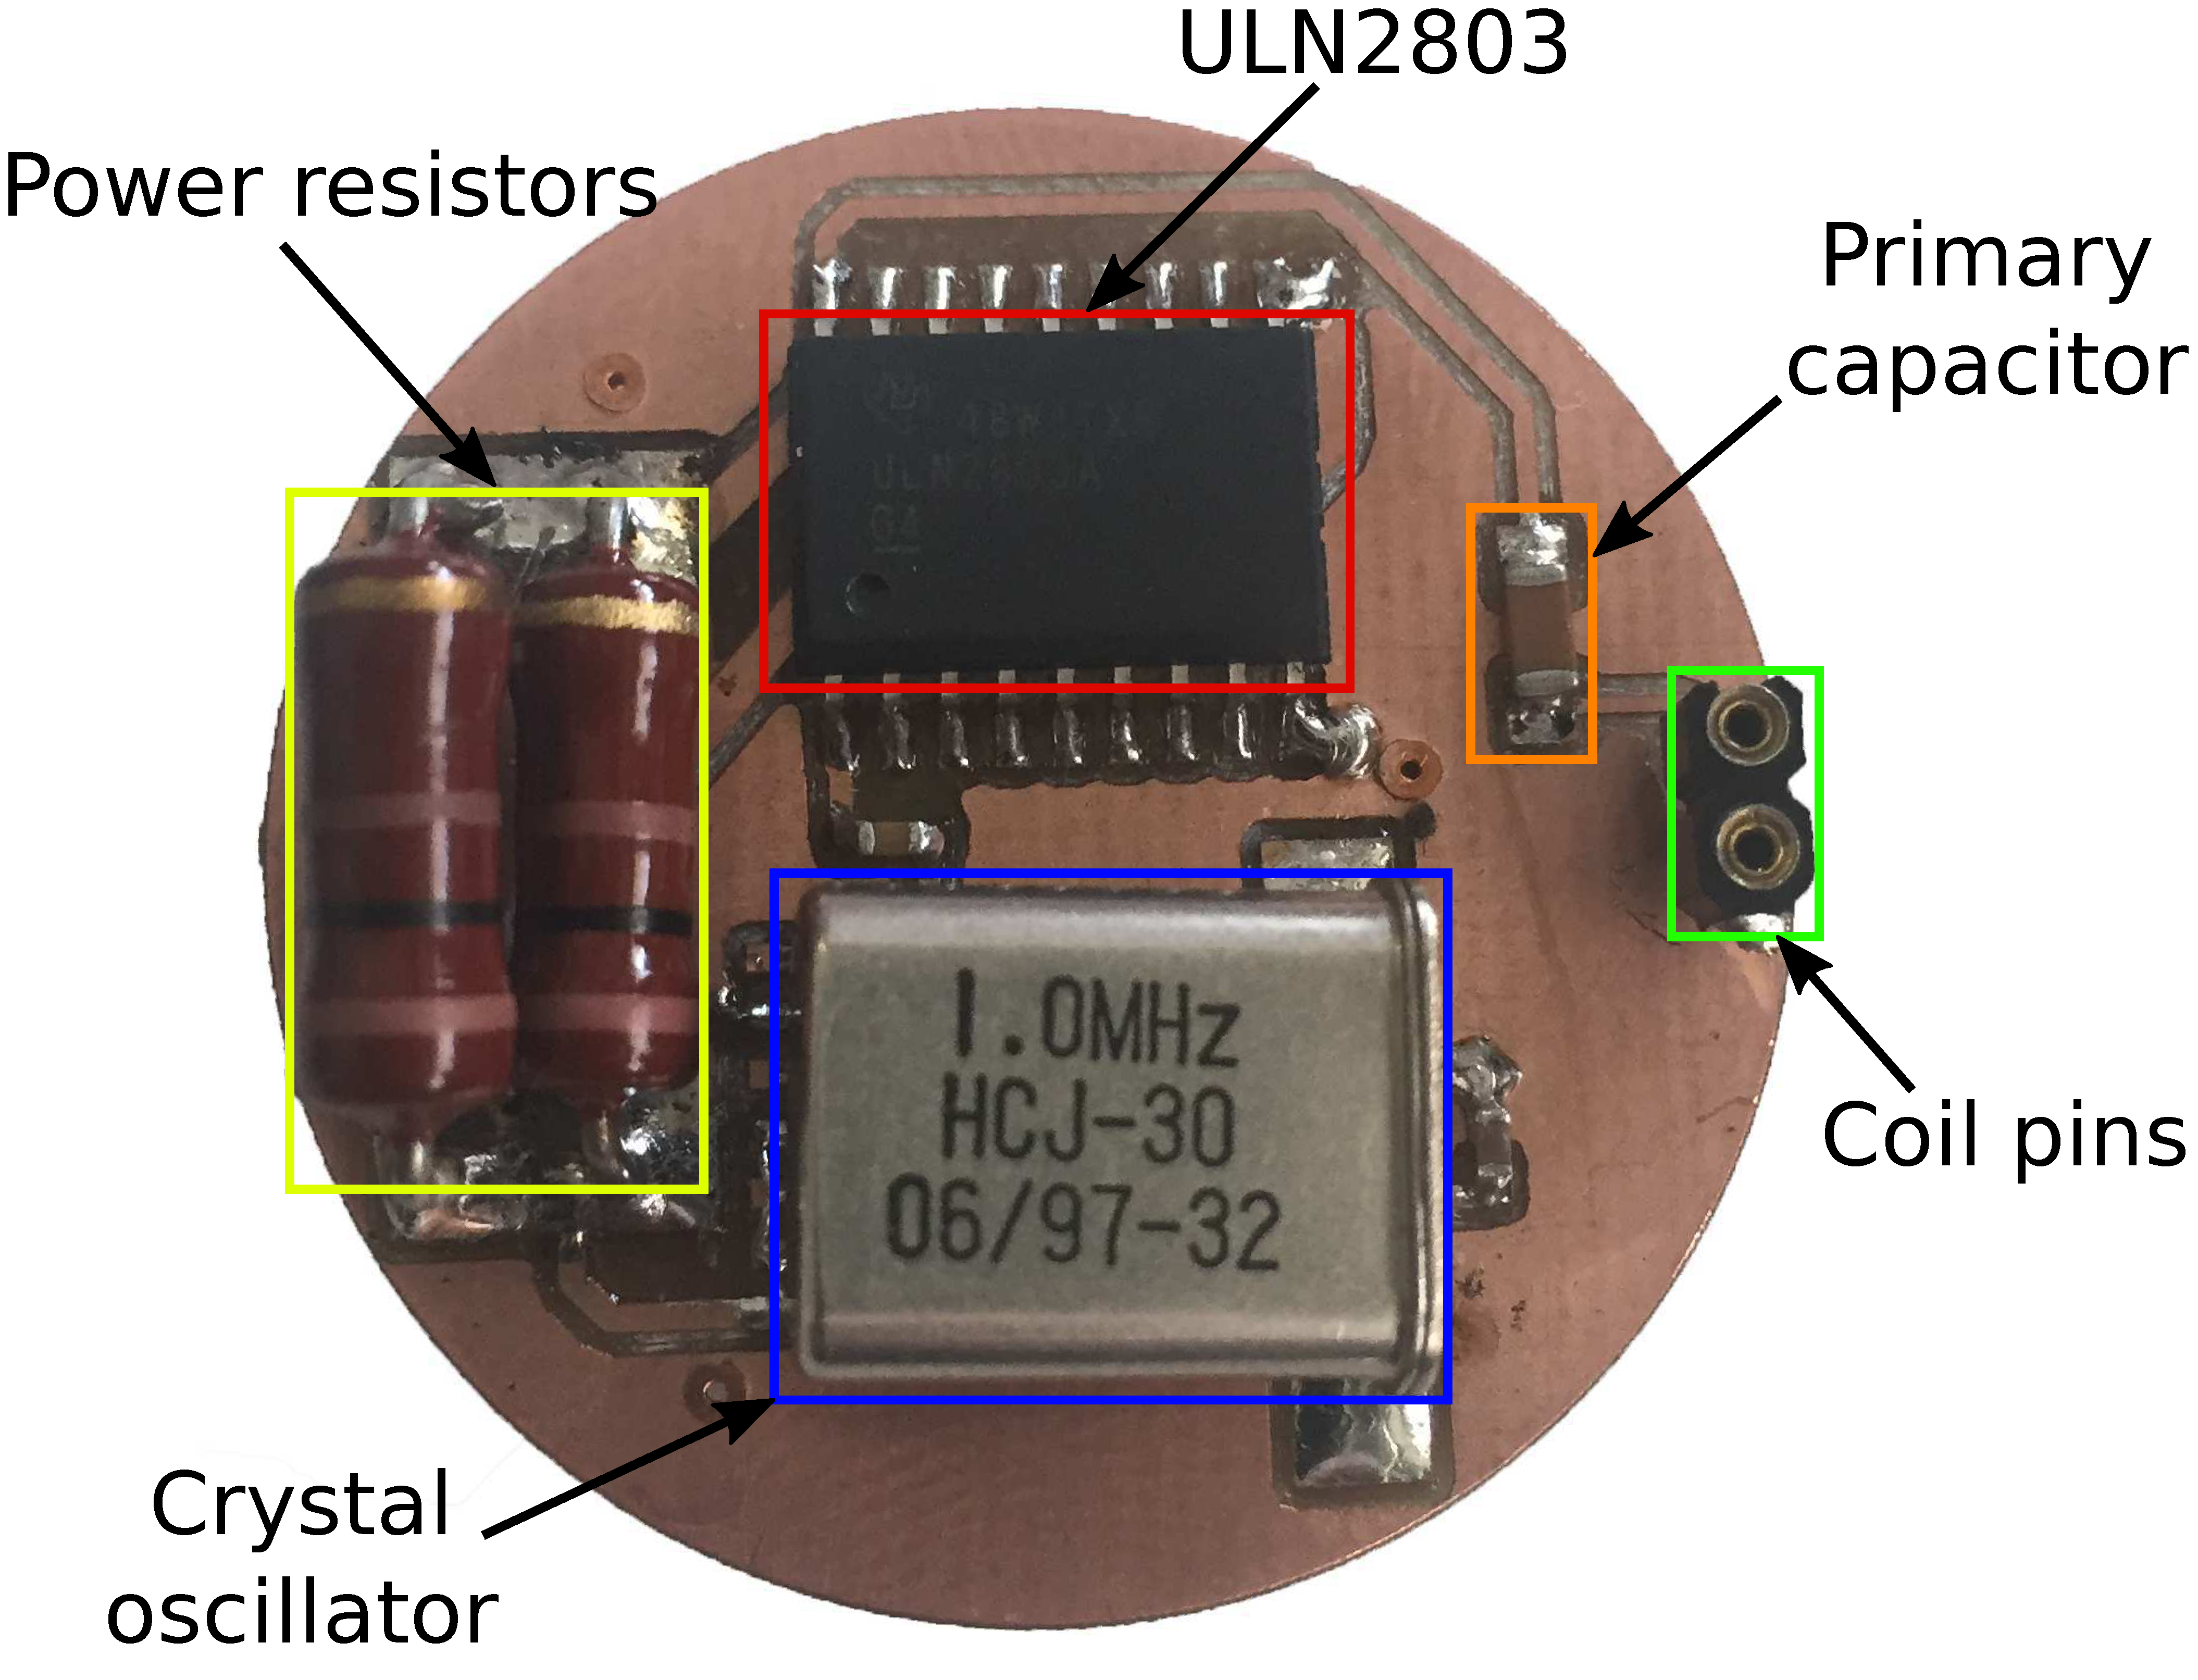
\includegraphics[width=2.0in]{./images/Transmitter_1X}\label{F:TX1}}\hfill
\subfigure[Side view] 
  {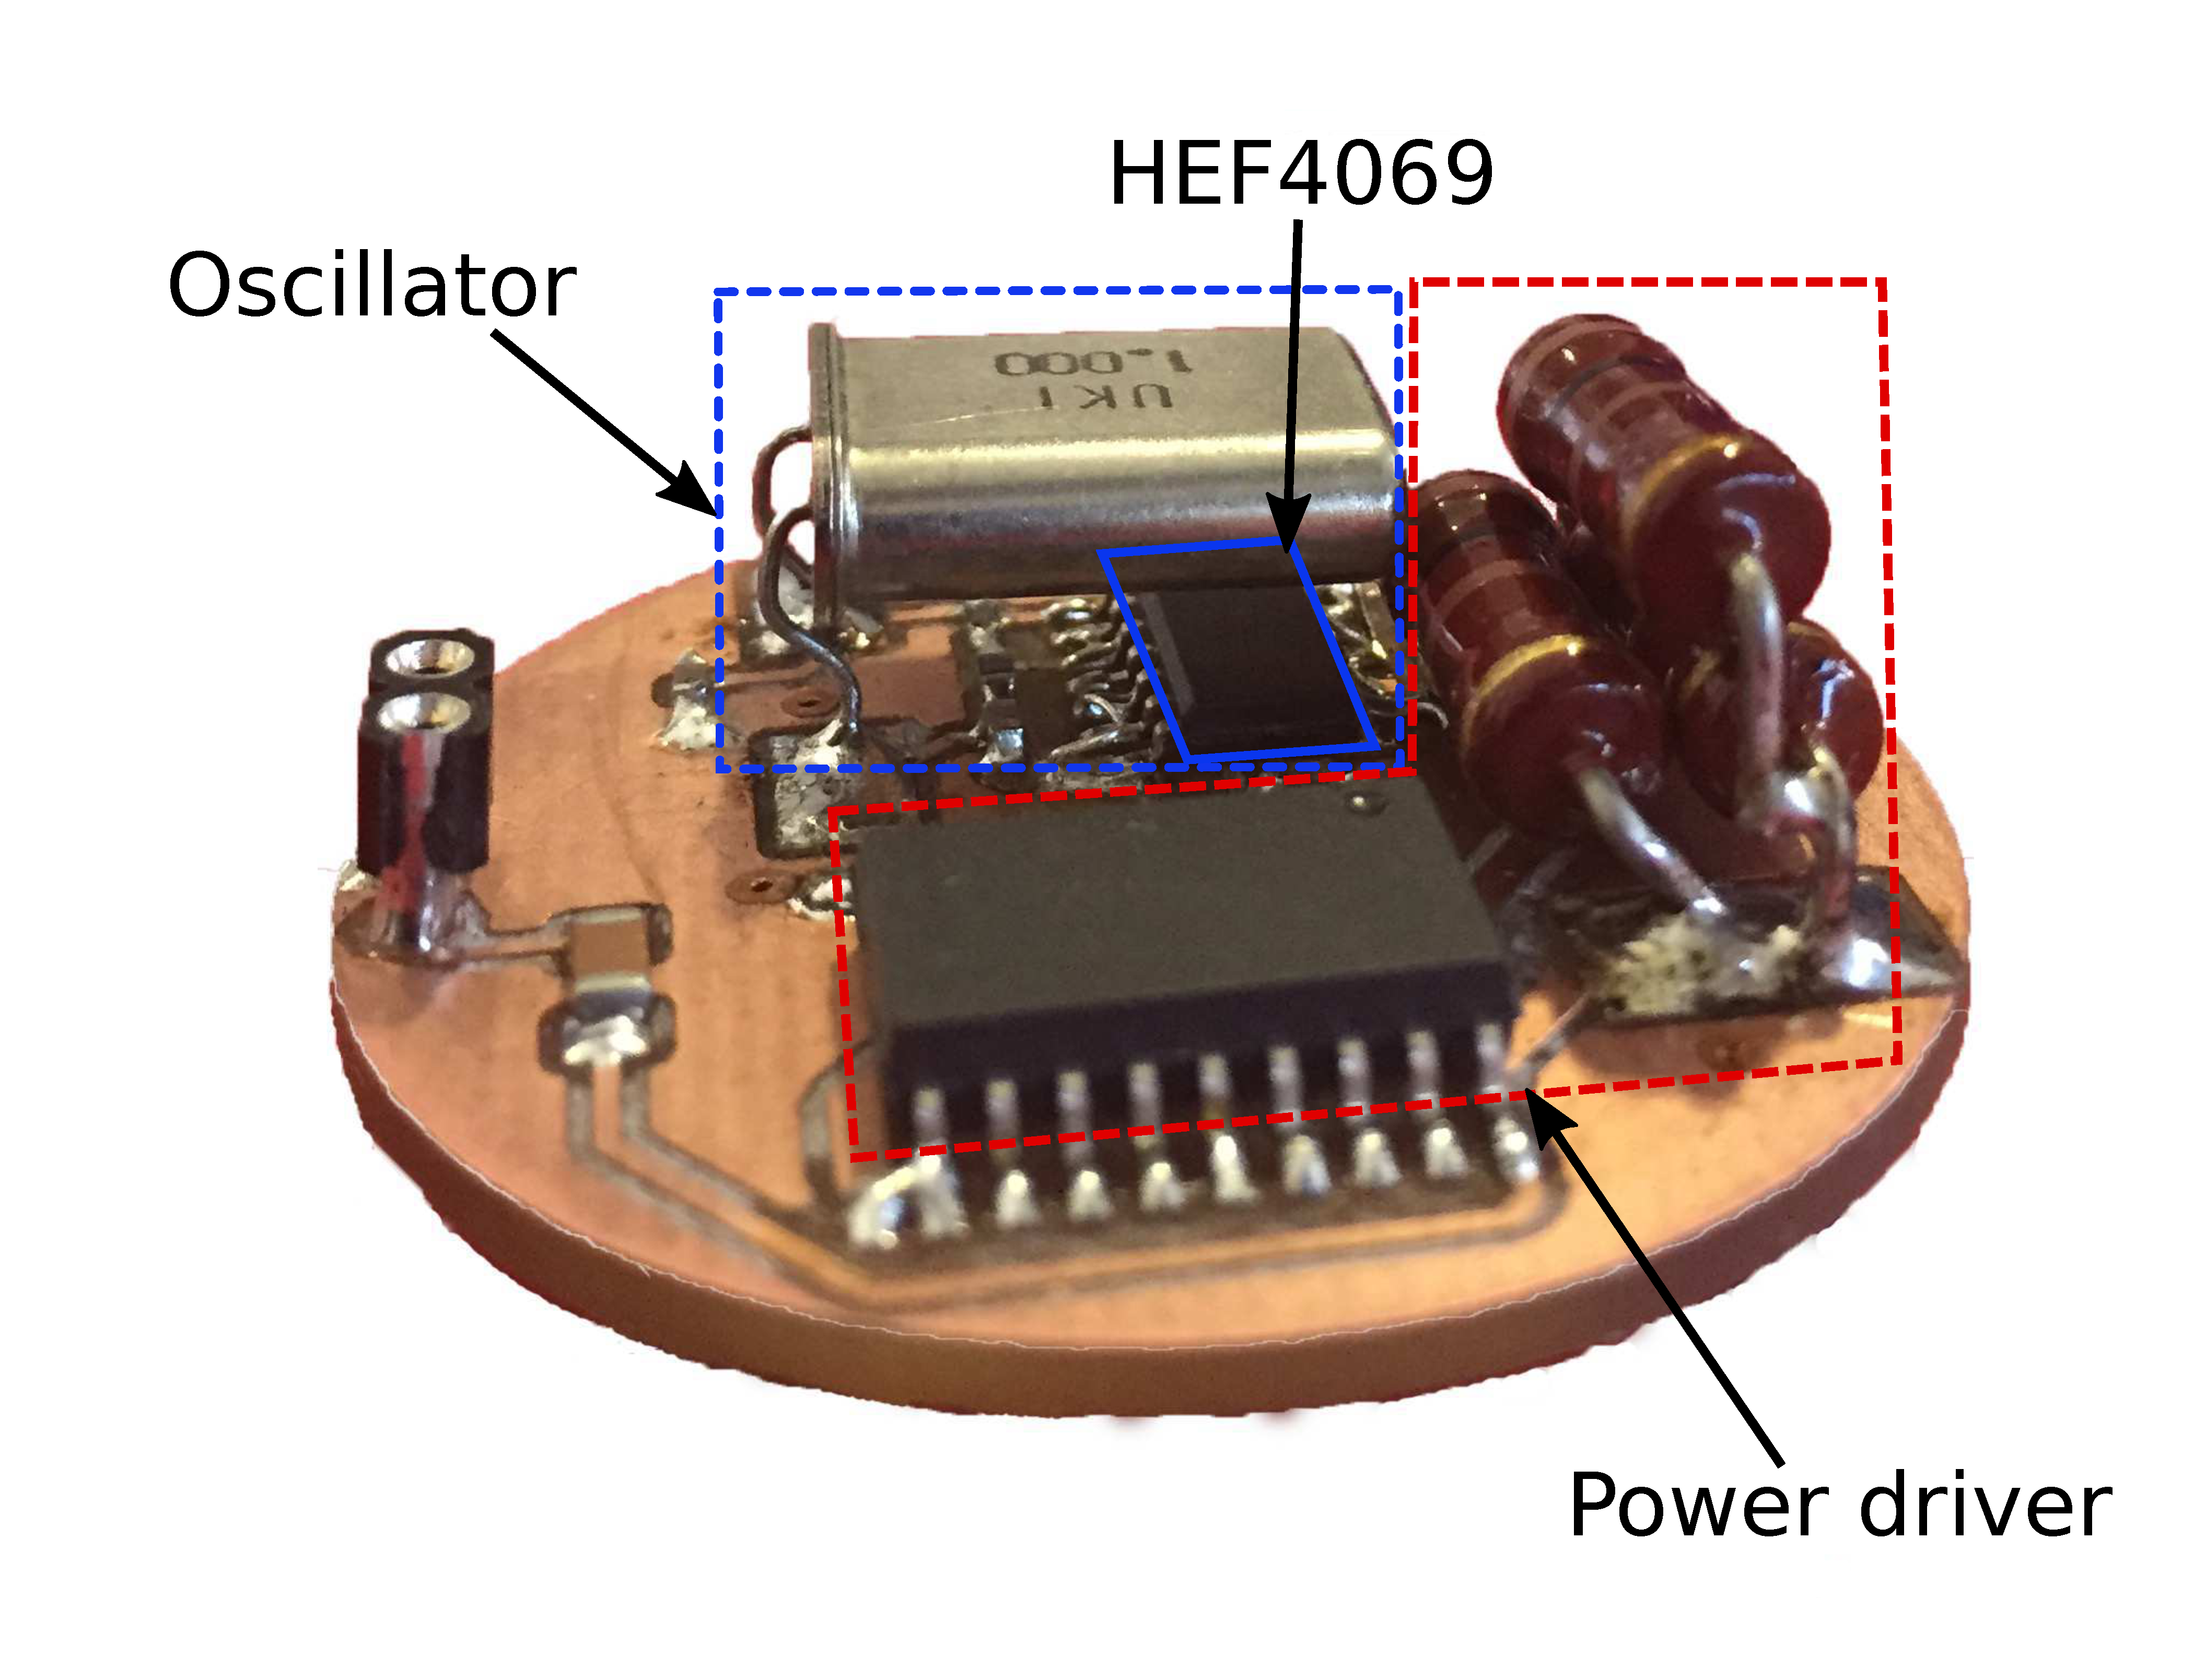
\includegraphics[width=2.0in]{./images/Transmitter_3}\label{F:TX3}}\hfill  
\subfigure[Back view]
  {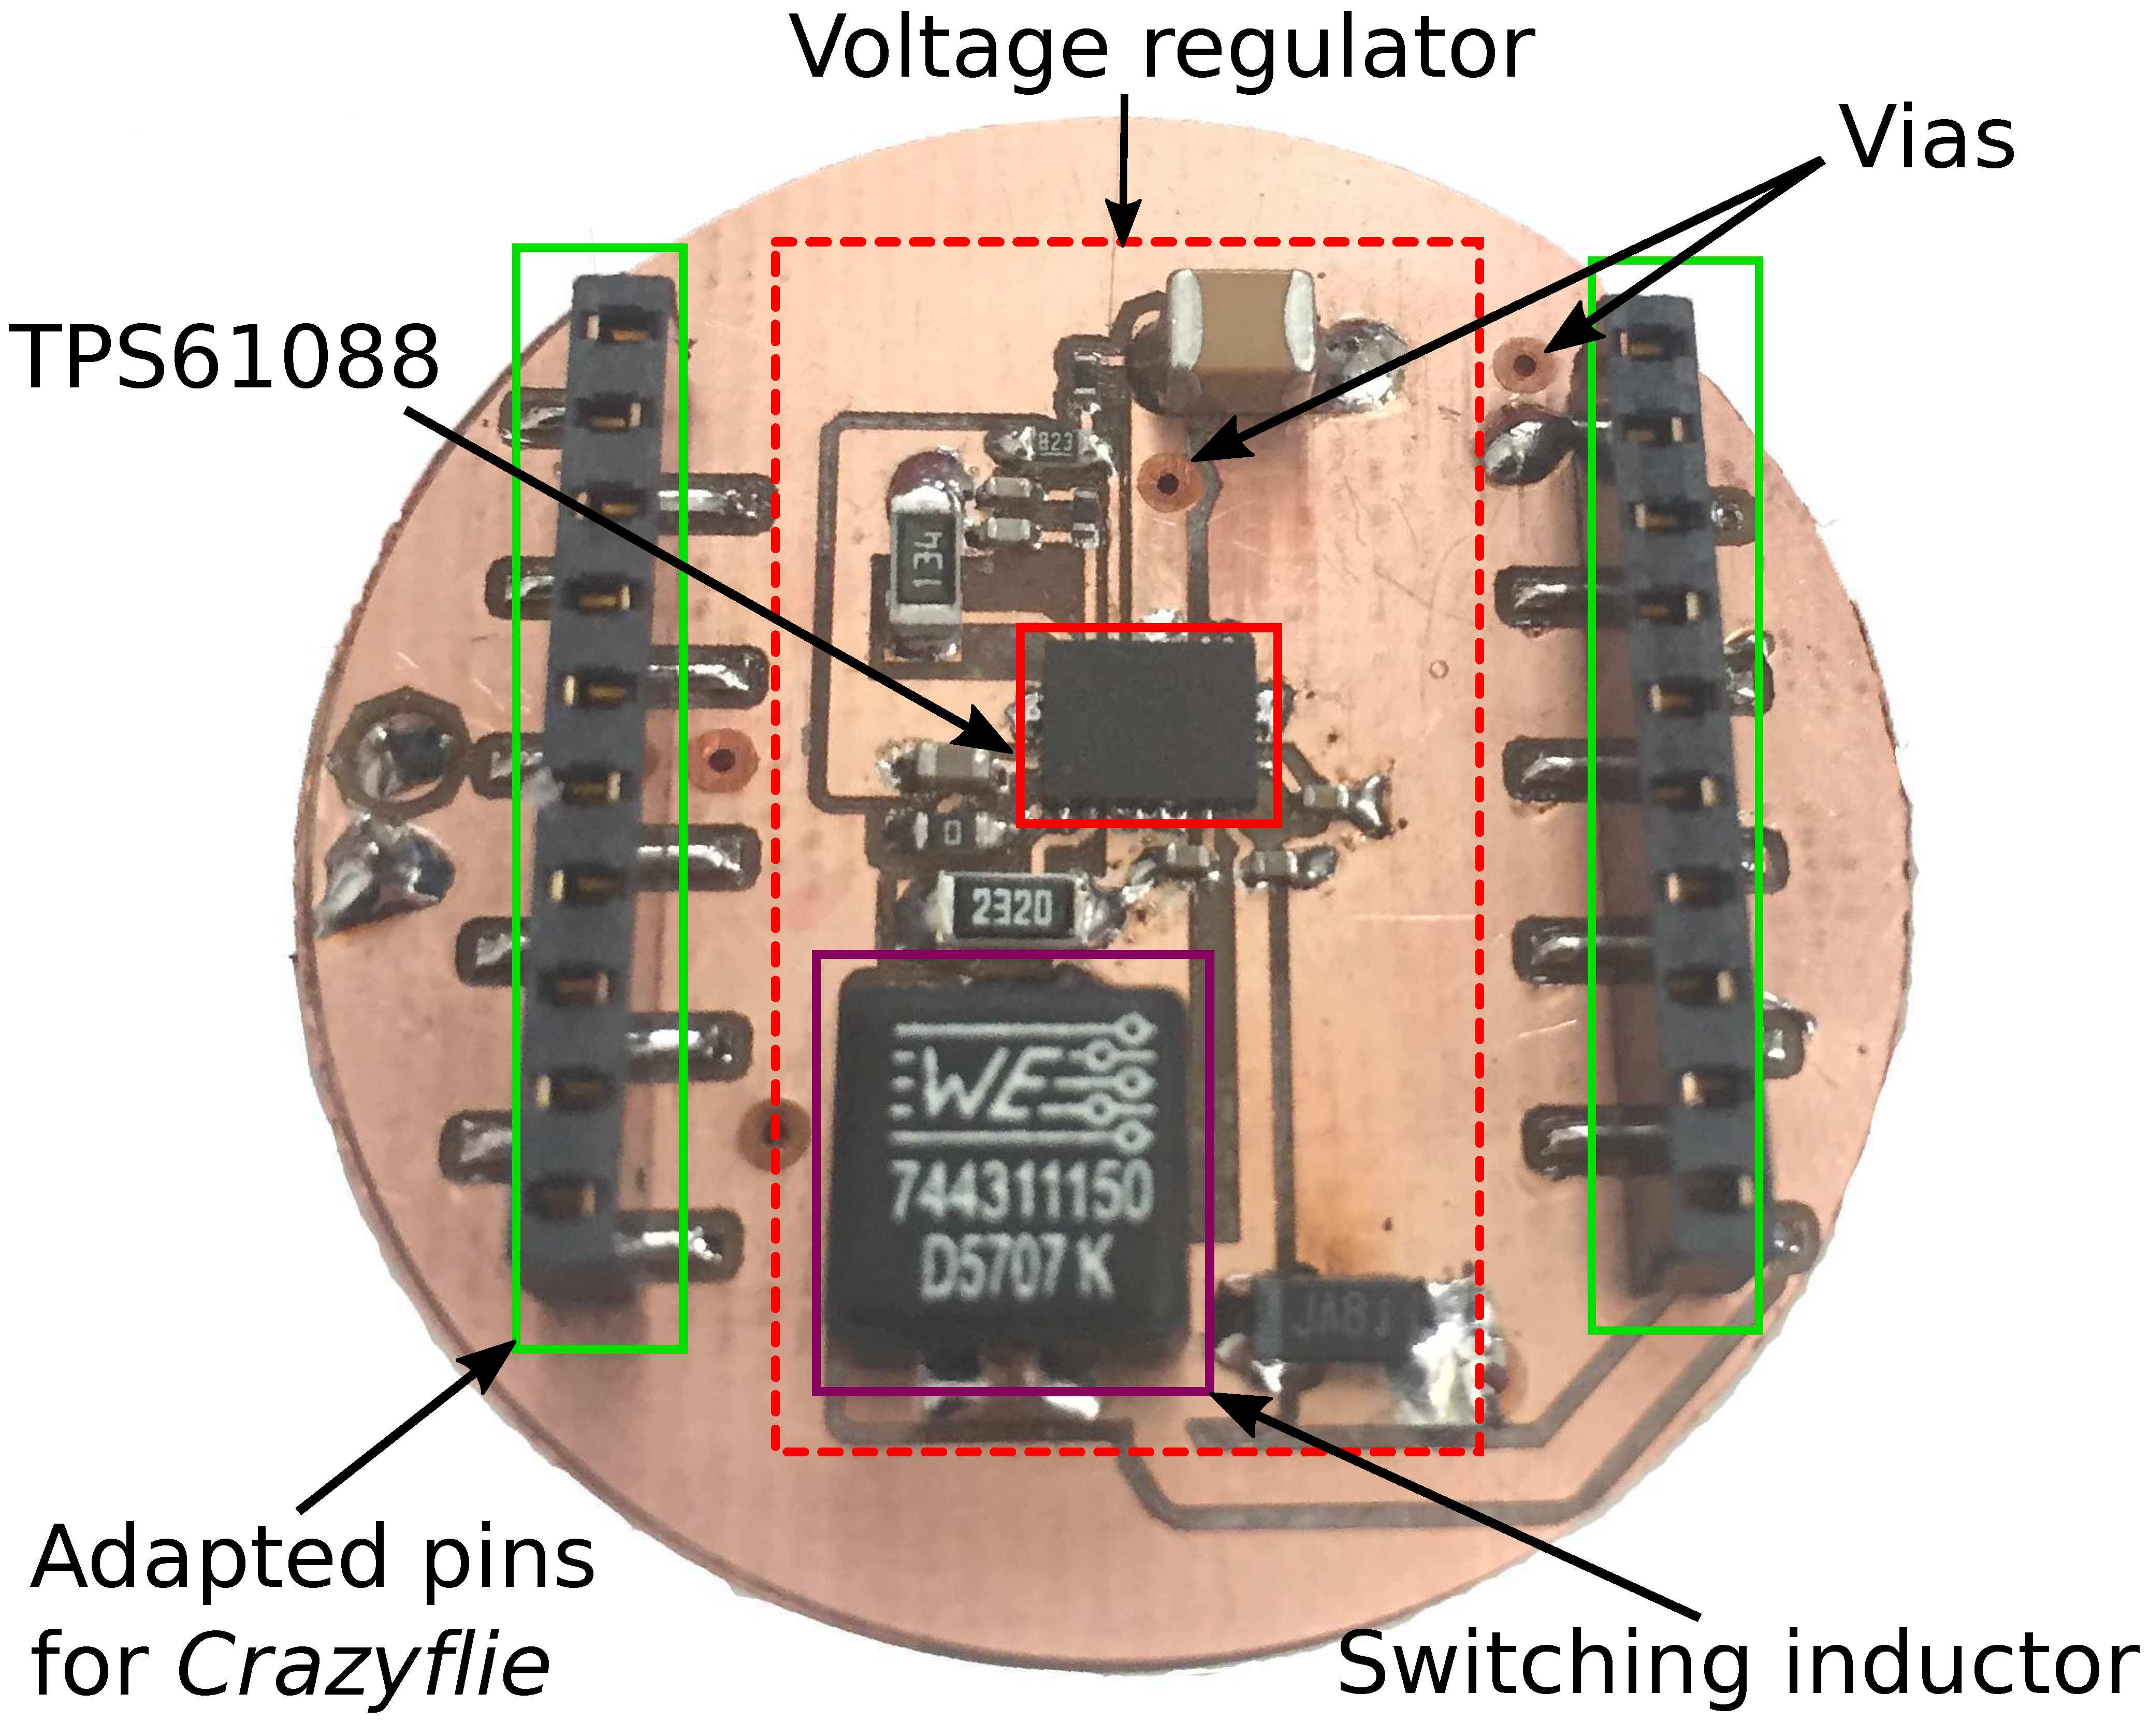
\includegraphics[width=1.9in]{./images/Transmitter_2Y}\label{F:TX2}}
\hspace*{\fill}%
\end{subfigmatrix}
\caption{Transmitter circuit}
\label{F:transmitter}
\end{figure}

Eventually, the total mass is computed using a precision scale. Table \ref{T:massConstraint} shows the mass of each section of the quadcopter. The experimental take-off mass depending on the motors thrust is shown in Figure \ref{F:thrust}. 

\begin{table}[htb]
\begin{center}
\begin{tabular}{|c|c|}

\noalign{\global\arrayrulewidth1pt}
\hline
\textbf{Element}  &   \textbf{Weight}\\
\hline
\hline
Battery             & 7.1 g     \\ \hline 
\textit{Tx} Coil    & 13.5 g    \\ \hline
\textit{Tx} Circuit & 8.5 g        \\ \hline
Crazyflie           & 8.3 g        \\ \hline
DC motors           & 4 x 2.8 g    \\ \hline
Motor mounts        & 4 x 0.8 g       \\ \hline
\hline
\textit{TOTAL}        & 51.8 g       \\ \hline

\end{tabular}
\caption{Mass constraint at transmitter side}
\label{T:massConstraint}
\end{center}
\end{table}


\begin{figure}[H]
  \begin{center} 
  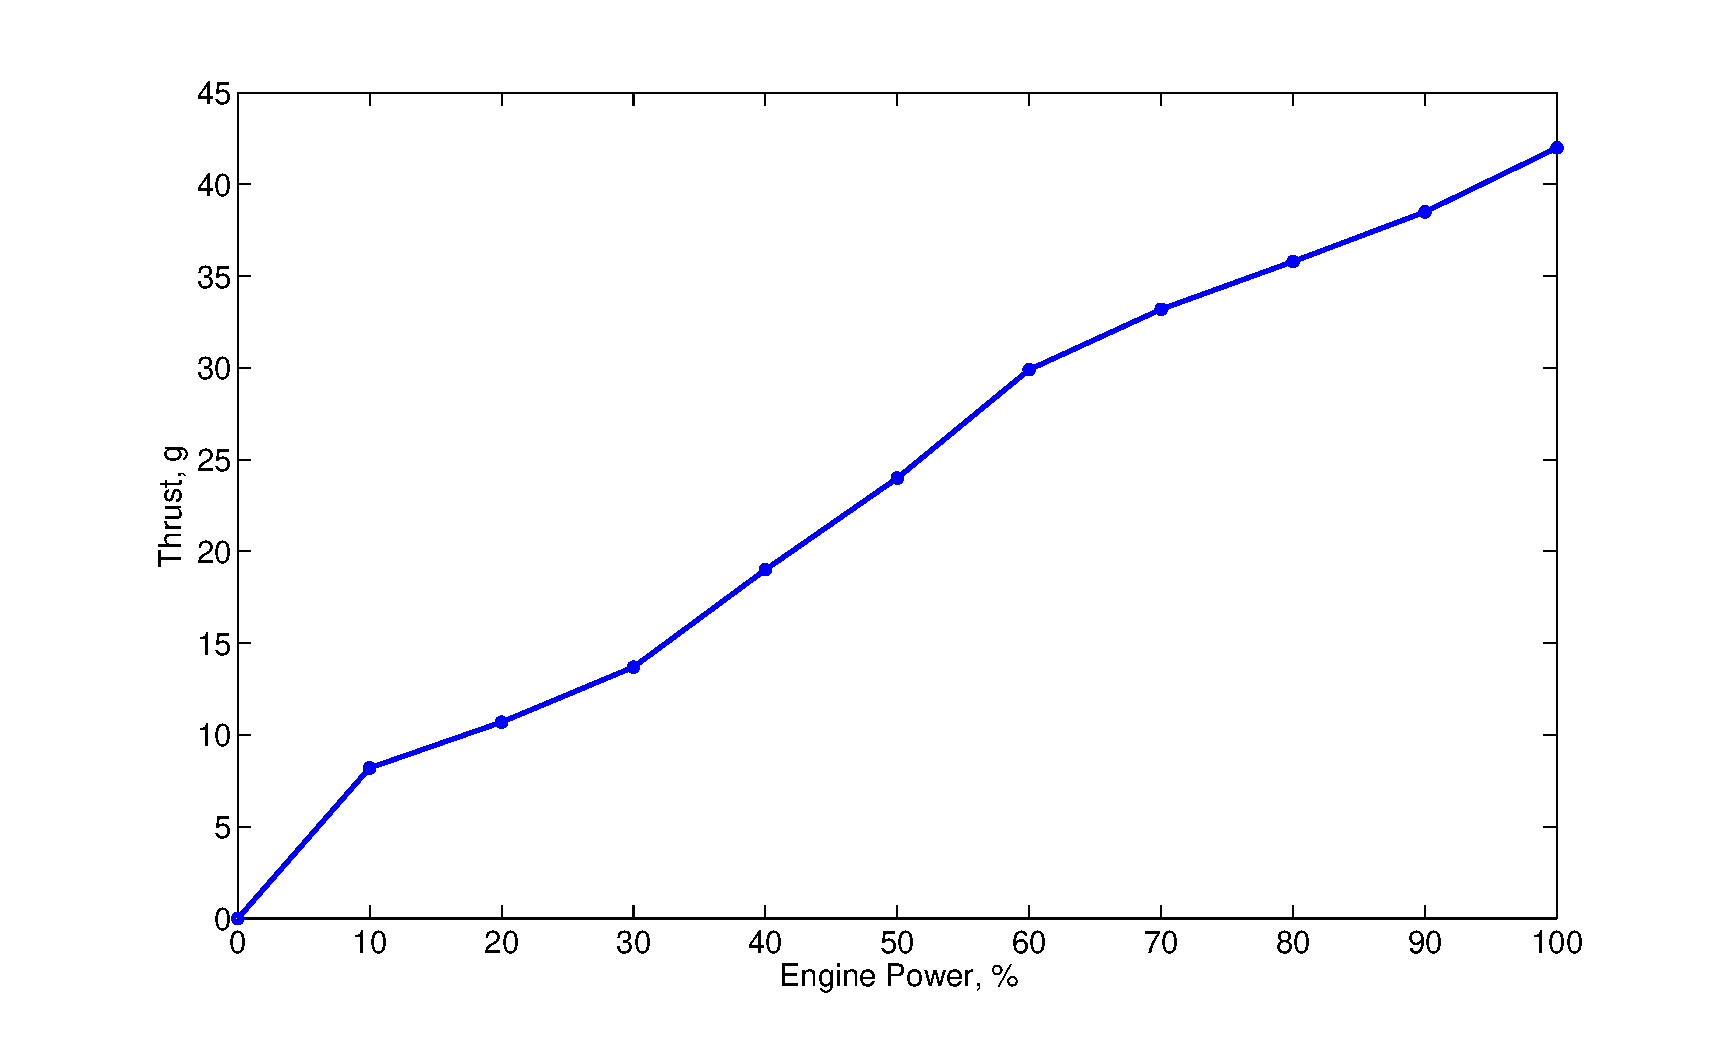
\includegraphics[width=0.9\textwidth]{./images/thrust}
    \caption{Thrust depending on the power level of the motors}
    \label{F:thrust}
  \end{center}
\end{figure}

\section{Receiver system}

The receiver side for a WPT system has the aim to rectify the transferred AC signal and, once it is in DC, to set it up to the desirable voltage levels. Depending on the application these two characteristic can be done in one stage. In the following sections the used circuits are explained in detail to accomplish a good signal rectification and conditioning. The chosen application for this project is presented is Section \ref{subsec:app}.

\subsection{Voltage Doubler}

To rectify the signal is selected a common used circuit for energy harvesting applications, the voltage doubler. This circuit is the perfect option for an energy harvesting. Owing to the low RF voltage levels, the doubler can rectify and condition at the same time. Voltage doubler circuits can be viewed as single stage or of a higher order multiplier; cascading identical stages together it is achieved a greater voltage multiplication. In Figure \ref{F:voltageDoubler} is shown a single stage for voltage doubler. 

\begin{figure}[ht!]
\begin{center}
\begin{circuitikz}
\ctikzset{v/.append style={/tikz/american voltages}}
\ctikzset{bipoles/resistor/height=0.25}
\ctikzset{bipoles/resistor/width=0.5}
\draw (0,2)
to[C=$C_1$] (2,2);
\draw (0,0)
to[short] (2,0)
to[D*] (2,2);
\draw (2,2)
to[D*] (4,2)
to[C=$C_2$] (4,0)
to[short] (2,0);
\draw (4,2)
to[short] (6,2);
\draw (4,0)
to[short] (6,0);
\node [ocirc] at (0,2) {$\qquad$};
\node [ocirc] at (0,0) {$\qquad$};
\node [ocirc] at (6,2) {$\qquad$};
\node [ocirc] at (6,0) {$\qquad$};
\node at (0,1) {$V_{in}$};
\node at (6,1) {$V_{out}$};
\node at (3,2.78) {$D_2$};
\node at (1.3,1) {$D_1$};
\end{circuitikz}
\caption{SIngle voltage doubler stage}
\label{F:voltageDoubler}
\end{center}
\end{figure}

An understanding of this circuit can be gained by interpreting firstly what occurs when the down swing of the AC current flows through the circuit. The diode $D_2$ blocks the current flow through $C_2$, but not the flow that goes across $C_1$. This current flow charges $C_1$ up to the same level of the AC voltage amplitude. Once the up swing of the AC voltage is reached, the voltage of both AC source and $C_1$ drop across $C_2$, charging it approximately twice the peak voltage of the AC signal \cite{doubler}.

As it is said in the first paragraph the voltage doubler is used in many energy harvesting applications, where the frequency goes from MHz to GHz. Thus, not all diodes are able to commute at these frequencies. The operating frequency of the inductive system of this project is set of 1 MHz and the selected diodes for assembling the voltage doubler are the HSMS-2850 Schottky diodes (SOT-23 Package) from \textit{Avago Technologies}:

\begin{figure}[htb]
\begin{center}

\includegraphics[width=0.2\textwidth]{./images/schottky}
\caption{SOT-23 Package for HSMS-2850 Schottky diode}
\end{center}
\end{figure}
The impedance of the HSMS-2850 diode can be linearly modeled as Figure \ref{F:schottky} shows \cite{doubler2}:

\begin{figure}[ht!]
\begin{center}
\begin{circuitikz}
\ctikzset{v/.append style={/tikz/american voltages}}
\ctikzset{bipoles/resistor/height=0.25}
\ctikzset{bipoles/resistor/width=0.5}
\draw (0,2)
to[R=$R_S$] (2,2)
to[vR=$R_j$] (4,2)
to[short] (8,2);
\draw (2,2)
to[short] (2,0)
to[C=$C_j$] (6,0)
to[short] (6,2);
\node [ocirc] (1) at (0,2) { };
\node [ocirc] (1) at (8,2) { };
\end{circuitikz}
\caption{Single voltage doubler stage}
\label{F:schottky}
\end{center}
\end{figure}

In this case $R_s$ and $C_j$ are the series resistance and the junction capacitance respectively, and $R_j$ has the following expression:

\begin{equation}
R_j = \frac{8.33\cdot{10^{-5}}\:n\:T}{I_b+I_s}
\end{equation}

where $n$ is the ideality factor, $T$ is the temperature in Kelvin degrees, $I_b$ is the externally applied bias current in amperes and $I_s$ is the saturation current. All this values, called \textit{SPICE}\footnote{\textit{SPICE} (Simulation Program with Integrated Circuit Emphasis) is a general-purpose, open source analog electronic circuit simulator.} parameters, are tabulated in Table \ref{T:SPICEparameters}.


\begin{table}[htb]
\begin{center}
\begin{tabular}{|c|c|c|}

\noalign{\global\arrayrulewidth1pt}
\hline
\textbf{Parameter}  &   \textbf{Units}  &   \textbf{HSMS-2850}\\
\hline
\hline
$C_j$            & pF  & $0.18$            \\ \hline 
$I_b$       & A &   $3\cdot{10^{-4}}$           \\ \hline 
$I_s$       & A &   $3\cdot{10^{-4}}$          \\ \hline 
$R_s$         & $\Omega $ &   $25$      \\ \hline
$n$         & $-$ &   $1.06$      \\ \hline
\end{tabular}
\caption{SPICE parameters for HSMS-2850}
\label{T:SPICEparameters}
\end{center}
\end{table}


The total impedance $Z_{diode}$ is given by:

\begin{equation}
Z_{diode} = R_S+\frac{R_j}{1+j\omega{C_j}R_j}
\end{equation}

In this project are used three stages for the design of the voltage doubler. This stages allows us to obtain good voltage levels at the output with good efficiency. Since, the more voltage doubler stages, the less efficiency.


\subsection{DC-DC boost converter}

The final stage introduced in the whole system is the \textit{bq25504 EVM}. As it is defined in its datasheet on the Appendices, the \textit{bq25504 EVM} is a ultra low power boost converter with battery management for energy harvester applications. This device is an evaluation module (EVM) programmed for deliver a 3.1 VDC maximum voltage (Over Voltage) for charging the storage element with a capacity larger than 100 $\mu$F. The supercapacitor or the battery allows the system to provide any peak currents that never would be obtained from the input source. 


The selection of the evaluation module is due to low power levels (among microwatts) needed to start converting the voltage to the programmed levels. The boost converter can be started with an input voltage lower than 330 mV. Below this level until 100 mV, it can operate but with more difficult. Once the 330 mV are reached, the boost converter will operate normally. This fact is called \textit{cold start}.

The following figure shows the schematic of the \textit{bq25504 EVM} and the output pins where the load and battery has to be placed:

\begin{figure}[H]
\begin{center}
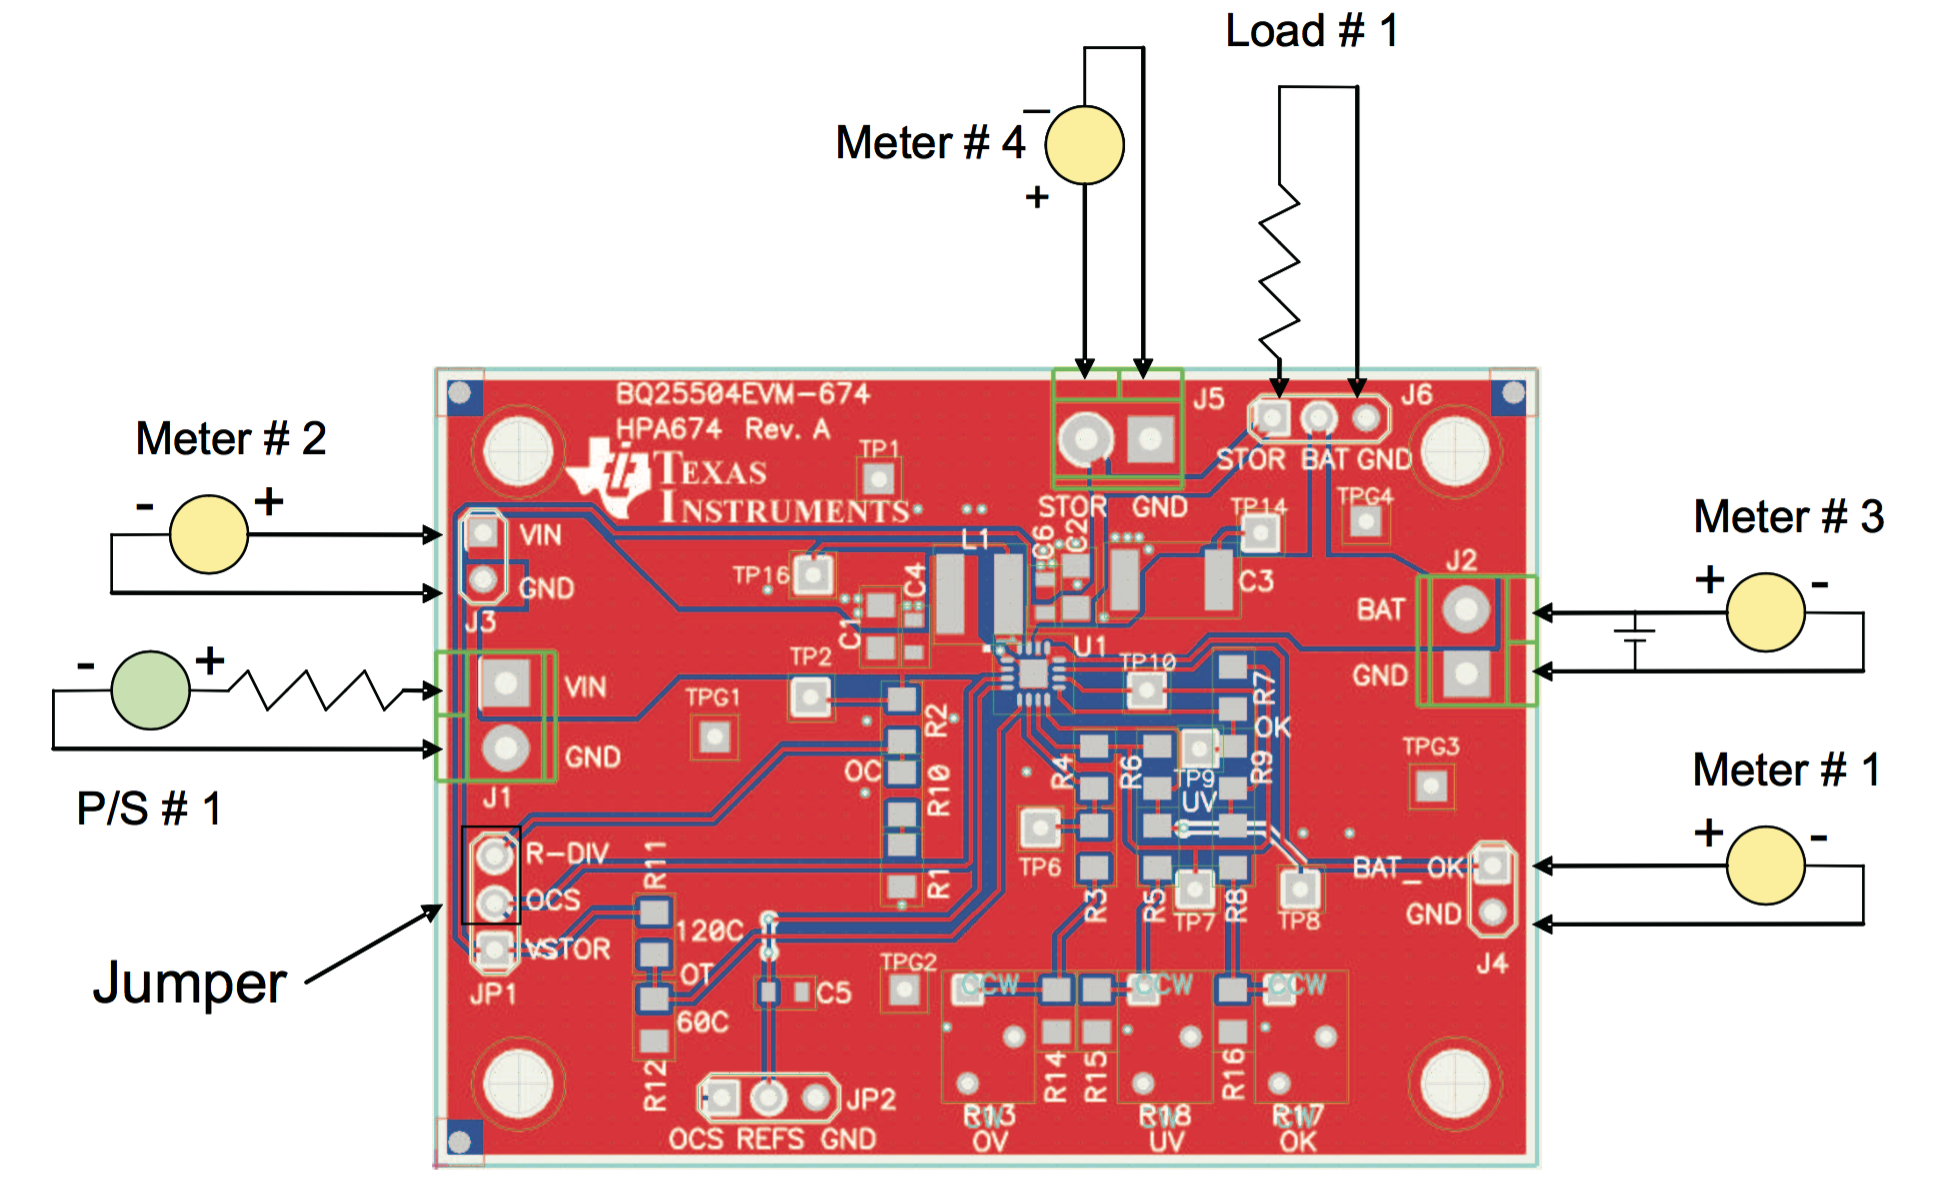
\includegraphics[width=0.8\textwidth]{./images/bq25504}
\caption{\textit{bq25504 EVM} schematic}
\end{center}
\end{figure}


\subsection{Storage element}

Included as a part of the \textit{bq25504 EVM}, the storage element has to be analyzed in detail because, depending on the used application and power source there are different options to select. The first constraint is based on the ability of the power source to provide enough voltage during a period of time to charge high capacity batteries or capacitors. In this project, the nano-quadcopter performances do not allow to charge this kind of storage elements in a small period of time. Thus, the storage element selection is reduced to batteries or capacitors up to 500 mF of capacity. 

The total energy stored in a battery or capacitor is given by:

\begin{equation}
E = \frac{1}{2}\:C\:V^2
\end{equation}    

where $C$ is the capacitance of the storage element and $V$ is the stored voltage. Imagine that the system consume 1 A and the storage element has a capacitance of 1 F and is charged with 1 V; assuming the following equations and doing some calculus,

\begin{equation*}
t = \frac{E}{P}  
\end{equation*} 

\begin{equation*}
P = V\:I
\end{equation*}
 
the system will provide this current consumption during 0.5 seconds.

By the previous considerations, it is possible to select the storage element used to run the application. The chosen supercapacitor is selected from \textit{AVX BestCap}, and it has 140 mF of capacitance. This capacitance is adequate, taking into account the system performances. Its capacitance can provide peak currents of about milliamperes without any problem in a short period of time and still supplying voltage.

\subsection{Application} \label{subsec:app}

Eventually, the definition of the used application to demonstrate the capability of the designed inductive transfer system is explained in this section. In a first instance, the purpose was to implement a low consumption sensor as a load. Usually, these sensors have a high constant consumption that prevents the battery last enough time. To solve this problem, it is used the \textit{eZ430-RF2500}. This device is a wireless developing tool with an integrated temperature sensor. An \textit{eZ430-RF2500T} target board is connected in the receiver and communicates with the other target board installed on a USB debugging interface to show the air temperature using the Sensor Monitor Visualizer Application provided by the manufacturer. 

\begin{figure}[htb]
\begin{center}
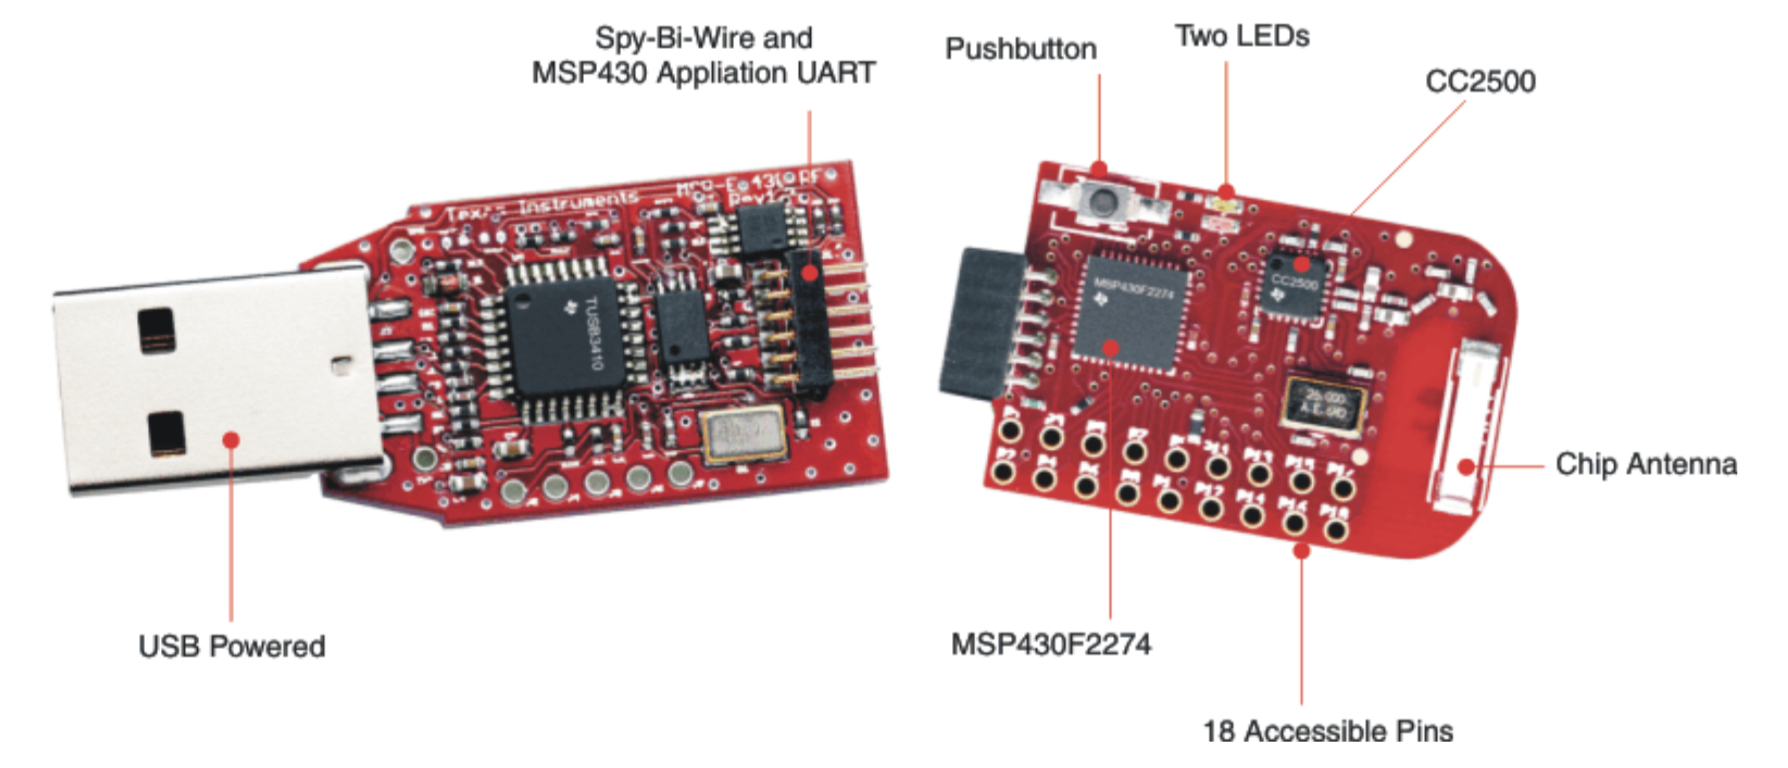
\includegraphics[width=0.8\textwidth]{./images/RF5000}
\caption{\textit{eZ430-RF2500} debugging interface (left) and target board (right)}
\end{center}
\end{figure}

The main advantage is that the device consumption, when is in active mode, is about 270 $\mu$A typically. The only drawback is that \textit{eZ430-RF2500} needs 21.2 mA to communicate with the \textit{CC2500} radio-frequency transceiver. This peak current can be easily supplied by the selected supercapacitor, mentioned in previous section. The device specifications are exposed in its datasheet, given in the Appendices.


\subsection{Receiver Circuit Assembly}

As the receiver is not constrained in mass, the assembling of this part has been done in a \textit{stripboard}. Its relative small size allows to locate everywhere depending on the developed application. The resulting receiver circuit is exposed in Figure \ref{F:receiverC}.

\begin{figure}[H] 
\begin{center}
\includegraphics[width=0.6\textwidth]{./images/receiver222}
\caption{Receiver circuit}
\label{F:receiverC}
\end{center}
\end{figure}
\chapter{Experimental Results} \label{C:experimental}
In this chapter the model is \textit{justified} using experimental information. Usually it is said to be the easiest part of model evaluation; whether it fits experimental measurements or not. Actually, it has been the most arduous task. Repetitive measures under different conditions, for each model, are carried out in order to validate the theoretical model.

Assumptions, simplifications and external factors made experimental results to separate from theoretical computations. Accepting this fact, the only intention is to get closer to resonant induction and be able to predict different behaviours depending on the input parameters selected.

	\section{Validations and Measurements}
In this section has been evaluated separately the resonant inductive system and the final WPT system outfitted on the drone. While in the inductive system is intended to validate the model without paying attention to the result values, in the second part these results and overall performance are discussed.


	\subsection{Resistance Estimation}
An accurate prediction of inductors' resistance is important when designing WPT systems, since it is some of the main factors that limit the power transfer capability and efficiency.

The resistance behaviour is constant until frequencies around 100 kHz. Then skin and proximity effects begin to increase the coil resistance value up to tens of ohms (\ref{F:LRvsF}). The test frequency selected to compute the theoretical values is 1 MHz. The measures on the 8 test coils are performed by using an HP 4294A Precision Impedance Analyser (40 Hz - 110 MHz). 


\begin{table}[ht]
\begin{center}
% \setlength{\tabcolsep}{12pt}
\begin{tabular}{c|c|c|r}

\noalign{\global\arrayrulewidth0.5pt}
\hline

\begin{tabular}{@{}c@{}}Coil 			\\ model 				\\								\\ $[-]$ \end{tabular} &
\begin{tabular}{@{}c@{}}Measured  		\\ resistance			\\								\\ $[\Omega]$ \end{tabular} &
\begin{tabular}{@{}c@{}}Calculated  	\\ resistance 			\\(using \ref{eq:Resistance}) 	\\ $[\Omega]$ \end{tabular} &
\begin{tabular}{@{}c@{}}Relative 		\\ error 				\\	$\epsilon_1$				\\ $[100\%]$ \end{tabular} \\

\noalign{\global\arrayrulewidth0.5pt}
\hline
\hline

$A_{Tx}$   & 0.5639 	& 	0.6519 	& 	13.49 	 	\\ \hline 
$A_{Rx}$   & 0.5916 	& 	0.6519 	& 	9.24  	 	\\ \hline 
$B_{Tx}$   & 0.6071 	& 	0.6193 	& 	2.00  	 	\\ \hline 
$B_{Rx}$   & 0.6380	 	& 	0.6193 	& 	2.93  	 	\\ \hline 
$C_{Tx}$   & 0.6704 	& 	0.6519 	& 	2.75  	 	\\ \hline 
$C_{Rx}$   & 0.6286 	& 	0.6519 	& 	3.70  		\\ \hline 
$D_{1}$    & 0.4485 	& 	0.2216 	& 	50.59 	 	\\ \hline 
$D_{2}$    & 0.3368 	& 	0.1306 	& 	61.22 		\\ \hline

\end{tabular}
\caption{Inductance calculation and measurement results}
% \label{T:K}
\end{center}
\end{table}

The results are in relatively good agreement with absolute errors smaller than 15$\%$ for the 3 candidate models. However, the theoretical resistances for models D1 and D2 are far from reality. This could be explained by the presence of AC effects when increasing frequency, and so a wrong modeling of the wire due to the varnish insulation (Table \ref{T:varnish}).




	\subsection{Inductance Estimation}
An accurate estimation of inductance is important because it is used to define the induction system model. It is also a vital parameter in tuning the resonant frequency of the WPT system. In Section \ref{subsec:coilInductance} there are defined different equations which approximate multiple-layer air-core coils.

The theoretical computations are validated through individual measures performed on the 8 test coils using an HP 4294A Precision Impedance Analyser (40 Hz - 110 MHz). The experimental values of inductance are measured in the frequency range of 10 kHz to 20 MHz. It must be said that inductance values behind 15 MHz start to behave strangely. 



\begin{table}[ht]
\begin{center}
% \setlength{\tabcolsep}{12pt}
\begin{tabular}{c|c|c|c|c|r}

\noalign{\global\arrayrulewidth0.5pt}
\hline

\begin{tabular}{@{}c@{}}Coil 			\\ model 				\\								\\ $[-]$ \end{tabular} &
\begin{tabular}{@{}c@{}}Measured  		\\ inductance			\\								\\ $[\mu\textnormal{H}]$ \end{tabular} &
\begin{tabular}{@{}c@{}}Calculated  	\\ inductance 			\\(using \ref{Eq:Wai}) 		\\ $[\mu\textnormal{H}]$ \end{tabular} &
\begin{tabular}{@{}c@{}}Relative 		\\ error 				\\	$\epsilon_1$				\\ $[100\%]$ \end{tabular} &
\begin{tabular}{@{}c@{}}Calculated  	\\ inductance  			\\(using \ref{Eq:Harold})			\\ $[\mu\textnormal{H}]$ \end{tabular} &
\begin{tabular}{@{}c@{}}Relative 		\\ error 				\\	$\epsilon_2$				\\ $[100\%]$ \end{tabular} \\

\noalign{\global\arrayrulewidth0.5pt}
\hline
\hline

$A_{Tx}$   & 12.45 	& 	12.38 	& 	0.56  	& 	11.21 	&	9.95 	\\ \hline 
$A_{Rx}$   & 12.46 	& 	12.38 	& 	0.64  	& 	11.21  	& 	10.03  	\\ \hline 
$B_{Tx}$   & 13.96 	& 	12.72 	& 	8.88  	& 	12.75 	& 	8.66  	\\ \hline 
$B_{Rx}$   & 13.7 	& 	12.72 	& 	7.15  	& 	12.75 	&	6.93 	\\ \hline 
$C_{Tx}$   & 13.67 	& 	13.26 	& 	2.99  	& 	12.60  	& 	7.82 	\\ \hline 
$C_{Rx}$   & 13.67 	& 	13.26 	& 	2.99  	& 	12.60 	& 	7.82	\\ \hline 
$D_{1}$    & 7.889 	& 	7.36 	& 	6.70  	& 	7.18  	& 	8.98  	\\ \hline 
$D_{2}$    & 4.25 	& 	4.42 	& 	4.00  	& 	4.37 	& 	2.82  	\\ \hline

\end{tabular}
\caption{Inductance calculation and measurement results}
% \label{T:K}
\end{center}
\end{table}

The results show good agreement with absolute errors smaller than 10$\%$ for Equation \ref{Eq:Wai}. The results of Equation \ref{Eq:Harold} are also quite good specially for model D2. All these computations have been performed for a test frequency of 1 Mhz. Note that inductance and resistance values are constant up to 500 kHz (see Appendix \ref{sec:RL}).


	\subsection{Quality Factor}
The experimental quality factor measurements of the coils reveal how \textit{good} the coils are for transferring energy. From Figure \ref{F:experimentalQualityFactor} it can be observed that all coils have similar Q factors, and it increases with the frequency. Hence, we will try to work at the highest possible operating frequency, which is constrained by the Equation \ref{eq:maxop}.

\begin{figure}[htb]
\begin{center}
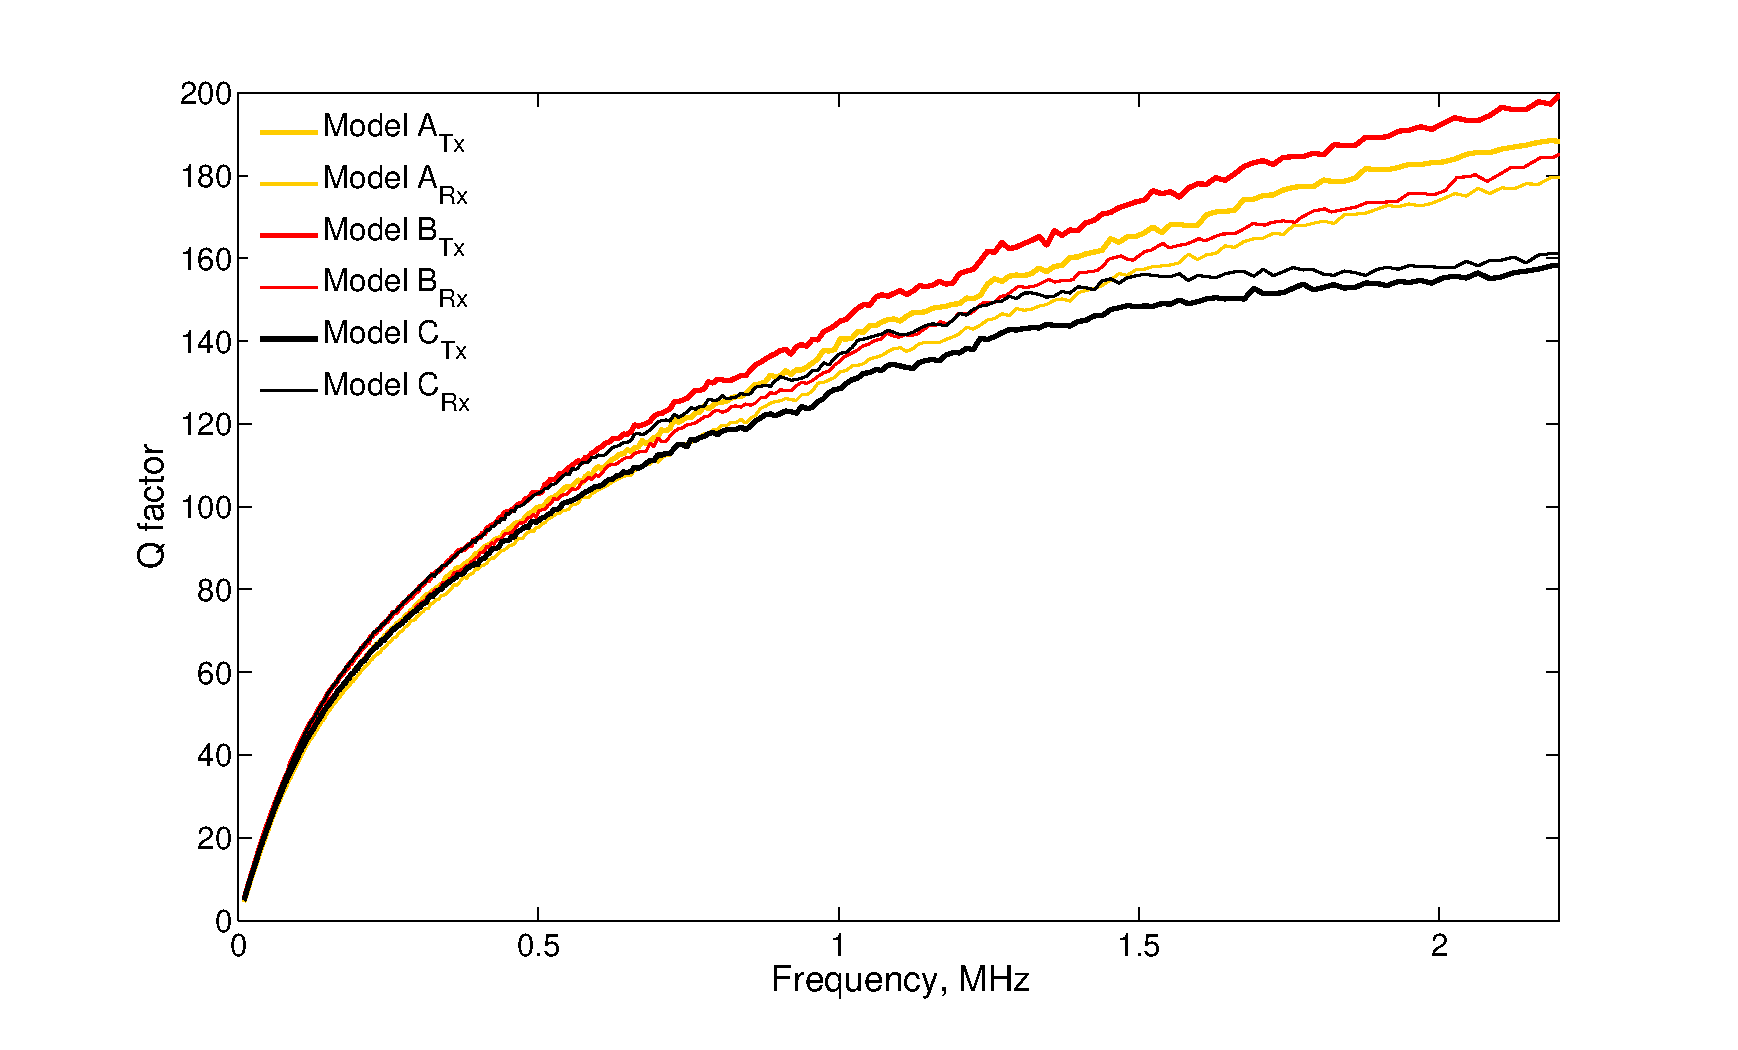
\includegraphics[width=1\textwidth]{./images/qualityFactor}
\caption{Experimental quality factor of model coils}
\label{F:experimentalQualityFactor}
\end{center}
\end{figure}

Table \ref{T:experimentalSelfFrequency} exhibits the self-resonant frequency of models A, B and C, as well as their operating frequency.

\begin{table}[htb]
\begin{center}
\begin{tabular}{c|c|c|c}

\noalign{\global\arrayrulewidth0.5pt}
\hline
Model  &   $f_s$ 	& $f_{op(max)}$ 	& Q factor\\
\hline
\hline
A      & 4.33 MHz 	 & 0.86 MHz	&      129   \\ \hline 
B      & 6.96 MHz 	 & 1.39 MHz	&      160   \\ \hline 
C      & 4.76 MHz    & 0.95 MHz&       125   \\ \hline 
\end{tabular}
\caption{Self-frequencies}
\label{T:experimentalSelfFrequency}
\end{center}
\end{table}

The Q factor values of the table above are computed for the operating frequency. It would have not been \textit{fair} to compute Q factor for the same frequency, owing to each coil has its characteristic self-resonant frequency. The complete Q factor plot with respect to the frequency is presented in Appendix \ref{F:QFactorAll}, which includes the coil models D1 and D2.


	\subsection{Inductive System Performance}
The inductive model verification and validation are performed in this part of the project. The obtained results are made with several laboratory measuring instruments that may influence in the experimental measurements. This involves the necessity of evaluate its influence in a detailed way to assure that the correct experimental value is measured.

		\subsubsection{Previous considerations}

To make the analytical measurements of the resonant inductive system and compare it with the model, it is mandatory to drive this circuit with a sinusoidal voltage source. The chosen source is the \textit{Agilent 33120A} waveform generator. This AC voltage source is selected to avoid the impedances and losses that can exist if the crystal oscillator is used as source (the overall transmission system), which its impedance and losses are more difficult to determine. Thus, the total impedance of the overall circuit depends on different stages. Working with this waveform generator we ensure having a impedance determined by the manufacturer.

The output voltage rating of the \textit{Agilent A33120A} is between 35.35 mV$rms$ to 7.071 V$rms$ and it has a fixed output impedance of 50 $\Omega$. The first important point to be taken into account is that the default setting for the function generator is to display the desired voltage as though terminated into a 50 $\Omega$ load.  As a consequence, whether the displayed voltage is set to 3.535 V$rms$, the measured voltage at the output of the generator will be of 7.071 V$rms$.

All voltage measurements are done with the \textit{Agilent DSO3062A} oscilloscope and the \textit{Agilent N2862A} probe. In this part appears the second and third important points to understand. The second one is related with the input resistance in parallel with the input capacitance of the oscilloscope probe. The problem appears when a capacitive component is measured. If this capacitance has its order of magnitude similar to the input capacitance of the oscilloscope probe (about 12 pF), the measurement may be erroneous because the input capacitance can not be negligible and they will be summed.

The last important consideration when a measurement is done is the called ``ground effect''. This effect appears when the oscilloscope is used to measure the voltage drop across a circuit element, where the probe impedance is set in parallel with this component and forces to generate another reference of the ground. The following elements will be short circuited and the displayed value on the oscilloscope will be wrong. To solve this problem, floating oscilloscopes such as \textit{Agilent U1604A} are used, allowing to cancel this ``ground effect''.

% \begin{figure}[ht!]
% 	\begin{center}
% 		\includegraphics[width=0.7\textwidth]{./images/oscilloscope} 
% \caption{``Ground effect'' schematic}
% \label{F:GroundEf}
% 	\end{center}
% \end{figure}

		\subsubsection{Measurements methodology}

Once the previous considerations are understood, the analytical measurements can be made. In this experiment exist four independent variables which condition the measures. These variables are the source voltage, the operating frequency, the distance and the load impedance. First of all, we set the AC voltage source in 1 V$rms$ displayed (2 V$rms$ measured). The selection of this output voltage is the one to ensure that the function generator can provide the necessary power to our system without any problem. In the case that the impedance becomes small, the output current will be limited, below its maximum, by the selected low level of voltage. The measurements are made with a sinusoidal wave for three different frequencies: 0.7 MHz, 1 MHz and 2 MHz. These frequencies are selected in order to compare the behavior of the system for different sinusoidal excitations. These selection of the voltage source and the frequency leaves two independent variables defined. 

All measurements are done for SS and SP topologies for the primary and secondary coils of the same model, to simplify the comparison with the theoretical model. The optimal way to transfer energy is when the resonant frequency is the operating frequency, thus, compensation capacitors are determined depending on the operating frequency for each coil model. Two kinds of analysis are made: the efficiency and power dependence between the distance and the load impedance, the other two independent variables. This two analysis will allow us to verify the model equations for the energy transmission system, in terms of magnetic induction, and the power transferred to the secondary side, in terms of the optimal load that matches with the primary circuit.

The comparison between the real efficiency and output power with their respective theoretical values will allow us to validate the model. To perform that, first of all it is required to determine the input power. The calculation of the input power is done by computing the AC current flowing through the primary side of the core-less transformer and multiplying it by the source voltage. The calculation of an AC current is not a trivial task because typical multimeters can measure \textit{RMS} magnitudes of AC waveforms up to 300 kHz approximately. The only option for computing the AC current is to place a small resistor\footnote{The small resistor up to 1 $\Omega$ is selected not to change the behavior of the system. Large resistors could be better for determining the dropped voltage and to compute the current in a more precise way, but they will change the measured values.} in series after the source voltage and measuring, with a floating oscilloscope, the dropped voltage in this resistor; using the Ohm's law it is possible to calculate the input current. The resistor value is set to 1 $\Omega$. 

Distance analysis are made by aligning the coils concentrically. The transmission range is set from 2.5 cm to 10 cm modifying the distance each 1.25 cm. Note that this range goes from the center of the primary coil to the center of the secondary one. The selected small amplitude voltage does not allow us to increment this range. The only parameter that is variable in this case is the distance, thus, it is necessary to fix the load impedance. As it is said in Section \ref{subsec:discussion2}, the SS topology works better with small load impedances and the SP topology, with high load impedances. At the end of the Section \ref{subsec:Model} it was explained that maximum transferred power is when $Z_R$ is equal to the primary circuit impedance. Knowing that this reflected impedance is dependent on the distance and the load impedance, for each distance will be a load impedance that maximizes this power. To simplify the measures, $Z_L$ is fixed for SS and SP topologies with 75 $\Omega$ and 200 $\Omega$ respectively. In Figure \ref{F:distance} is exposed the analytical measuring procedure for a distance analysis.

The analysis with the load resistance are made by setting fixed the distance in 5 cm. For SS topology, the load is changed up to 100 $\Omega$ approximately and for SP topology, up to 7 k$\Omega$. This procedure is shown in Figure \ref{F:load}, where the two coils are distanced 5 cm.

\begin{figure}[htb]
\begin{center}
\begin{subfigmatrix}{2} 
\subfigure[Distance analysis]
{\includegraphics{./images/DistanceAnalysis}\label{F:distance}} 
\subfigure[Load analysis]
{\includegraphics{./images/LoadAnalysis}\label{F:load}}
\end{subfigmatrix}
\caption{Measuring procedure}
\label{F:procedure}
\end{center}
\end{figure}

In Appendix \ref{D1D2} it is demonstrated that an increment in \textit{Rx} radius is preferred upon the same increment in \textit{Tx} radius which was stated in Section \ref{finTFG}. This means that larger receivers allow higher power levels for a certain distance.

\subsubsection{Results}

The obtained results for all coil models are exposed in Appendix \ref{Appendix: experimental}. The distance and load resistance analysis results are quite close to the theory. The differences are due to the tolerance of the laboratory measuring instruments used. Another factor that roughly affects to the comparison between the reality and the theory is the losses due to the transmission through the air, which is the main reason of having losses. Nevertheless, the tendency of the real measures is almost the same as theoretical values curves.

	\subsection{Overall System Performance}

To complete the experimental results, the overall system performance has to be analyzed. As it has said in Chapter \ref{C:architecture}, the used coil model for the overall system is the Model C. Thus, the experimental results are obtained by analyzing some interesting points corresponding to Model C performances.

The first test was to determine the autonomy of the nano-quadcopter battery using the transmitter circuit coupled to the receiver, and charging the super capacitor without the load installed. The methodology for this test was to put the nano-quadcopter at 2.5 cm from the receiving coil using the SS topology. The full charging of the super capacitor is reached at exactly 10 minutes with the nano-quadcopter battery without being discharged. As Figure \ref{F:battery2} shows, the nano-quadcopter's  battery is completely discharged after 16 minutes approximately. The blue dashed line indicates the voltage limit where the inductive system is turned off. This limit corresponds to the minimum voltage allowed by the regulator to boost the voltage level to 12 VDC. This voltage is experimentally selected to accomplish measurable power levels in the receiver, at a distance of 20 cm.

\begin{figure}[htb]
\begin{center}
\includegraphics[width=0.8\textwidth]{./images/battery2}
\caption{Nano-quadcopter's battery discharging profile}
\label{F:battery2}
\end{center}
\end{figure}

It has been proved the same test with the SP topology and the charge time is increased over 14 minutes. The conclusion of this fact is that the load impedance (that is difficult to determine in this part of the project) could be relatively small (above 50 $\Omega$). This means that the optimal topology to use is the SS compensation topology.

Once it has tested that the nano-quadcopter can charge the super capacitor, the same experiment is done by installing the \textit{eZ430-RF2500} target board. As it has expected, the system is not able to manage the charge of the super capacitor and to run the \textit{eZ430-RF2500} at the same time. The reason is that the \textit{CC2500} RF transceiver needs to communicate with the other target board, installed on a PC for running the Sensor Monitor Visualizer Application, consuming the 21.2 mA when the battery has the equivalent energy to this current. As a result, this sensor will not communicate to its receiver and the battery will not be charged; a voltage controlled switch (like a NMOS circuit) or a push button, such as in our case, has to be implemented.

The push button (see Figure \ref{F:receiverC}) allows the nano-quadcopter to charge the battery and, when the battery is charged to the minimum voltage that can provide the enough energy for supply 21.2 mA, the push button can be triggered in order to feed the sensor. Figure \ref{F:overall} shows the realized experimental procedure for this section. In the figure it can be seen both the computer and the sensor target boards are displayed on the screen showing their temperature respectively.


\begin{figure}[H]
\begin{center}
\includegraphics[width=0.8\textwidth]{./images/overall}
\caption{Overal system measurement.}
\label{F:overall}
\end{center}
\end{figure}

Table \ref{T:finalfinal} exhibits the comparison between the theoretical and analytical power consumption.

\begin{table}[H]
\begin{center}
\begin{tabular}{c|c|c|c|c}

\noalign{\global\arrayrulewidth0.5pt}
\hline
Source voltage  &   Theoretical current & Theoretical power	& Consumed current & Consumed power 	\\
\hline
\hline
3.7 V     & 1.05 A & 3.88 W	 & 1.06 A  & 3.92 W  \\ \hline 

\end{tabular}
\caption{Consumption comparison}
\label{T:finalfinal}
\end{center}
\end{table}

\cleardoublepage
\phantomsection
\chapter*{Conclusions}




%%%  BIBLIOGRAFIA
%%%%%%%%%%%%%%%%%%%%%%%%%%%%%%%%%%%%%%%%%%%%%%%%%%%%%%%%%%%%%%%%%%%%%%%%%%

%%% Per la bibliografia hi ha 2 opcions: generarla amb la utilitat BibTeX 
%%%                                      o fer-la ''a ma''
%%% NOTA: podeu trobar facilment informació sobre BibTeX a:
%%%  http://www.ctan.org/tex-archive/biblio/bibtex/contrib/doc/

%%% OPCIO 1: BibTeX (recomanat) -> descomentar les comandes seguents:

% unsrt
% unsrtnat
% plainnat
% natbib
% plain
% bibtex
% unsrturl

\bibliographystyle{unsrturl}   %% Estil de bibliografia EETAC unsrt
\cleardoublepage
\phantomsection
% Indicar aqui el(s) fitxer(s) que contenen la bibliografia

\bibliography{biblio} 
\pdfbookmark{Bibliografia}{sec:biblio}

%%% OPCIO 2: bibliografia manual
%%%
%%% L'argument d'entrada es el numero de referencies que s'inclouen
\cleardoublepage
\phantomsection
%\begin{thebibliography}{2}

%% Llibres:  Autor/s (cognoms i inicials dels noms), títol del llibre (en cursiva), editor, ciutat i any de publicació. Quan es cita el capítol d'un llibre s'ha d'indicar el títol del capítol (entre cometes), el títol del llibre (en cursiva) i els números de pàgines amb la primera i la darrera incloses.

%%  Exemple de capitol en llibre
% \bibitem{prova1} 
% Cognoms-autor, Inicial-nom.
% ``Títol del capítol''. {\it Títol del llibre}.
% (Editor. Ciutat. Any publicació): pagina1--paginaN.

% %%  Exemple de d'article en revista
% \bibitem{prova2} 
% Cognoms-autor, Inicial-nom.
% ``Títol de l'article''. {\it Títol de la revista}.
% {\bf volum}(numero),
% pagina1--paginaN. (Any publicació) 

%\end{thebibliography}

%%%%%%%%%%%%%%%%%%%%%%%%%%%%%%%%%%%%%%%%%%%%%%%%%%%%%%%%%%%%%%%%%%%%%%%%%%
%%%%%%                           APENDIXS                         %%%%%%%%
%%%%%%%%%%%%%%%%%%%%%%%%%%%%%%%%%%%%%%%%%%%%%%%%%%%%%%%%%%%%%%%%%%%%%%%%%%
\pagestyle{empty}  % no tocar

%% Descomentar una de les dues línies següents, en funció de:
%%  a) els apendixs s'encuadernaran apart (amb portada) 
%%  b) els apendixs s'enquadernen amb el mateix projecte (sense portada). 
%% Recordeu que si tot el document (amb apèndixs) excedeix les 100 pagines 
%% s'ha d'enquadernar a part
%\appendix\ambportada
%\appendix\senseportada


%%%%%%%%%%%%%%%%%%%%%%%%%%%%%%%%%%%%%%%%%%%%%%%%%%%%%%%%%%%%%%%%%%%%%%%%%%
%%%%%% INCLOURE A PARTIR D'AQUI TOTS ELS CAPÍTOLS DELS APENDIXS   %%%%%%%%
%%%%%%%%%%%%%%%%%%%%%%%%%%%%%%%%%%%%%%%%%%%%%%%%%%%%%%%%%%%%%%%%%%%%%%%%%%

%%%%%%%%%%%%%%%%%%%%%%%%%%%%%%%%%%%%%%%%%%%%%%%%%%%%
\chapter{Inductance Characterization}\label{Appendix: AA}
\section{Inductance Estimation Table}



\section{Equivalent coil impedance} \label{AppendixSection: impedance}






%%%%%%%%%%%%%%%%%%%%%%%%%%%%%%%%%%%%%%%%%%%%%%%%%%%%
%%%%%%%%%%%%%%%%%%%%%%%%%%%%%%%%%%%%%%%%%%%%%%%%%%%%
%%%%%%%%%%%%%%%%%%%%%%%%%%%%%%%%%%%%%%%%%%%%%%%%%%%%
%%%%%%%%%%%%%%%%%%%%%%%%%%%%%%%%%%%%%%%%%%%%%%%%%%%%
\chapter{Model equations} \label{Appendix: A}
\section{Secondary capacitor in series} \label{sec:secondaryS}



\section{Secondary capacitor in parallel}\label{sec:secondaryP}

The same steps as above are followed for obtaining the impedances $Z_2$ and $Z_R$ when the secondary capacitor is placed in parallel: 


%%%%%%%%%%%%%%%%%%%%%%%%%%%%%%%%%%%%%%%%%%%%%%%%%%%%
%%%%%%%%%%%%%%%%%%%%%%%%%%%%%%%%%%%%%%%%%%%%%%%%%%%%
%%%%%%%%%%%%%%%%%%%%%%%%%%%%%%%%%%%%%%%%%%%%%%%%%%%%







%%%%%%%%%%%%%%%%%%%%%%%%%%%%%%%%%%%%%%%%%%%%%%%%%%%%
\chapter{Coils Experimental Results}
\section{Inductance and Resistance}\label{sec:RL}




\section{Quality Factor}








%%%%%%%%%%%%%%%%%%%%%%%%%%%%%%%%%%%%%%%%%%%%%%%%%%%%
%%%%%%%%%%%%%%%%%%%%%%%%%%%%%%%%%%%%%%%%%%%%%%%%%%%%
\chapter{Circuit Schematics}

\section{Voltage Regulator}\label{Appendix: DC-DC}

% \begin{figure}[htb]
% 	\begin{center}
% 		\includegraphics[width=1.05\textwidth]{./images/TPS61088}
% 	\caption{TPS61088 design circuit}
% 	\end{center}
% \end{figure}




%%%%%%%%%%%%%%%%%%%%%%%%%%%%%%%%%%%%%%%%%%%%%%%%%%%%%%%%%%%%%%%%%%%%%%%%%%
%%%%%%%%%%%%%%%%%%%%%%%%%%%%%%%%%%%%%%%%%%%%%%%%%%%%%%%%%%%%%%%%%%%%%%%%%%
%%%%%%%%%%%%%%%%%%%%%%%%%%%%%%%%%%%%%%%%%%%%%%%%%%%%%%%%%%%%%%%%%%%%%%%%%%
\end{document}
